% \documentclass[12pt]{siamltexmm} 
\documentclass{article}
\usepackage{amsmath} 
\usepackage{amscd}
\usepackage{amssymb}
\usepackage{amsfonts}
\usepackage{amsthm}
\usepackage{amsfonts}
\usepackage{amsthm}

\usepackage{circuitikz}
\usepackage{pgf}
\usepackage{tikz}
\usetikzlibrary{arrows,snakes,backgrounds}
% \usetikz

\usepackage{algpseudocode}
\usepackage{algorithm}
\usepackage{subfig}

\usepackage[super]{nth}
% \usepackage{appendix}
% \usepackage{listings}
% \usepackage{color} 
\usepackage{ulem}
\usepackage{hyperref}
%\usepackage{url}
\usepackage{cancel}
\usepackage{cleveref}

\usepackage{aviolov_style}
\usepackage{local_style} 
\def \tf {{t_f}}
\def \topt {{ t_{opt}}}


\begin{document}
\title{Optimal Design for Estimation in Diffusion Processes from
First-Hitting-Times}
\author{Alexandre Iolov, Susanne Ditlevsen, Andr\'e Longtin  \\
$<$\href{mailto:aiolo040@uottawa.ca}
		{aiolo040 at uottawa dot ca}$>$, alongtin at uottawa dot ca}

\date{\today}

\maketitle  

\abstract{
We consider the optimal design problem for the Ornstein-Uhlenbeck process with
fixed threshold, commonly used to describe a leaky, noisy integrate-and-fire
neuron. We present a solution to the problem of devising the best external
time-dependent perturbation to the process in order to facilitate the estimation
of the characteristic time parameter for this process. The optimal design
problem is constrained here by the fact that only the times between
positive-going threshold crossings, known as hitting times, are observable. The
optimal control is based on a maximization of the mutual information between the
posterior of the unknown parameter given these observations and the distribution
of the hitting times.}     
 
% Keywords: Stochastic Optimal
% Control, Mutual Information, Leaky Integrate-and-Fire neuronal models,
% Fokker-Planck equation, Adjoint Method


\tableofcontents

% TODO: remove list of tables, figures
\listoftables  

% TODO: when settled on figures - make pretty
\listoffigures

\section{Introduction}
Techniques to extract dynamical parameters from observations of a stochastic
process is an active area of research. Generally one hopes to have access to
measurements of the state variable at a sufficiently high rate to guide the
estimation of these parameters. However, in some cases these states are not
measurable, and one has to work instead only with times at which specific events
occur, such as an earthquake or an epileptic seizure. Here we consider the
problem of optimal design for estimation of parameters in a stochastic
differential equation (SDE) given only observations of "hitting" times, i.e. of
times at which the process crosses a fixed threshold. And more specifically,
since a primary motivation is the activity of neurons, in our study these
hitting times are associated with positive-going crossings of a threshold
voltage. This corresponds to so-called extracellular potential measurements,
which exhibit a spike of a given shape when the voltage inside the cell has
crossed the threshold. While our motivation is based in neuroscience, the
technique we develop is more generally applicable to simple dynamical models
from which a point process can be extracted.

We assume that the 'controller' has influence over some part of the parameters
of the SDE, and that the objective is to obtain observations, in our context
these are hitting times, that are most informative in both formal and informal
senses. That is, we choose the control as the solution to a
well-posed optimization problem, but our ultimate goal is to obtain more
accurate and more precise estimates of the unknown parameter(s).

We espouse a Bayesian perspective and proceed by assuming a prior
distribution of the unknown parameters. Then we seek to maximize the Mutual
Information (MI) between the posterior of the unknown parameters given the
observations and the distribution of the hitting times. We note that, even for a
fixed and known parameter set, the hitting time observations 
are still random due to the inherent stochasticity of the SDE. 

Using Mutual Information for the selection of 'maximally informative'
experiments has been advocated by several recent lines of research, for example,
in experimental psychology, \cite{Cavagnaro2010,Myung2013}, computational
neuroscience \cite{Paninski2006a,Paninski2005,Lewi2009} and quantum physics,
\cite{Granade2012}. An alternative approach is to maximize the Expected Fisher
Information of the experiment, as in \cite{Hooker2015}. This is especially
effective if the Fisher Information is available as an analytical formula. That
is the case when one observes full trajectories from the diffusion process, as
in \cite{Hooker2015}, but not in the much more limited context of observations
of hitting-times. 
 
The Mutual Information measures the expected reduction in uncertainty in the
parameter value given an observation, under a fixed experimental stimulation.
Thus the stimulation that maximizes the Mutual Information should extract the
maximum information about the model's parameters, on average. Using Mutual
Information for estimating statistical quantities is formally justified; see
e.g. \cite{Paninski2005} where it is proven that, under fairly weak modeling
conditions, using a stimulus input that maximizes the mutual information between
future observations and the parameters of interest leads to consistent and
efficient parameter estimates. More generally, while theoretically sound,
optimizing or even merely computing the Mutual Information may be
computationally prohibitive. however, for our problem of interest, the primary
issue is the low level of information available given that one has only access
to hitting times, rather than measurements on an analog state variable.

We should explicitly single out a very recent paper \cite{Granade2012} that
describes a strategy to experimentally estimate the parameters of the
Hamiltonian of a quantum system. The qubit state outcomes of zeroes or ones
follows a Bernoulli distribution whose parameter is sought, and the time at
which observations are made is under experimental control. They use a simple
filtering technique originally suggested by \cite{Liu2001} to maintain and
update the prior distribution of the unknown parameters. In principle, their
approach is very similar to ours, the main difference is the nature of the
observations, which in our case are the hitting times.

As posed our optimization problem reduces to a slightly non-standard Partial
Differential Equation (PDE) optimization problem, in particular a
Fokker-Planck optimization problem. The field of PDE optimization is vast 
and we just mention one of many good
references, \cite{Borzi2012}. A series of papers on
Fokker-Planck based PDE-optimization has also appeared, e.g. \cite{Annunziato2010,Annunziato2014}.
None of these however deal with the boundary-based term that arises in our case out of the
hitting-time based objective. We should also mention our own \cite{Iolov2014a},
where we again solve a hitting-time inspired optimization problem. The
fundamental difference here is that the uncertainty in the model parameters
in the work below complicates the problem as it requires the solution of a system of
(loosely-) coupled PDEs (the number depending on the form of the prior
distribution), rather than just one as in \cite{Iolov2014a}. That work, as the
one below, are part of growing efforts to control nerve cells (see
e.g. \cite{Ullah2009})

Our paper is also part of the general literature on estimating parameters of
diffusion processes from hitting-times observations only. Partly due to the
applications of this problem in theoretical neuroscience a lot has been written
on the subject, for example in
\cite{Ditlevsen2007,MullowneyIyengar2008,Alili2005} as well as our own work
\cite{Iolov2013} where we deal with the more exotic case of a sinusoidal driving
force. The literature on estimation from hitting-times of the class of diffusion
models we consider asserts that one parameter in particular, the characteristic
time (i.e. the time constant of the Ornstein-Uhlenbeck process), is the most
difficult to estimate, and has by far the widest confidence bounds. Thus we
focus on devising an input control that will provide the most accurate estimates
for this parameter, assuming that the other parameters are known or at least
nominally known in a sense that we explain below.

Thus our paper can be summarized as solving a PDE-optimization arising from
maximizing the Mutual Information between a prior of the characteristic time
parameter and the random (future) hitting-times. Its outline is as  follows:  in
\cref{sec:problem_formulation} we describe the mathematical formulation of the optimal design problem; in
\cref{sec:maximizing_MI}, we describe the optimization procedure, in particular
the derivation of the objective gradient and the numerical methods used; in 
\cref{sec:sim_study} we discuss the general shape of the optimal solution and
its dependence on the various parameters in the model and the robustness of the
optimization algorithm; in \cref{sec:batch_estimation}, we show the performance
of the optimally designed stimulation when many observations are first collected and only a single-pass,
{\sl batch} estimation is performed afterwards; in \cref{sec:online_estimation},
we turn to the {\sl online} problem, where the estimation is performed
after each observation and the stimulation is adjusted to reflect the newly
updated prior of the unknown parameters; in \cref{sec:discussion} we make
concluding and forward-looking remarks. 
 
\section{Model}
\label{sec:problem_formulation}
Consider a noisy, leaky integrate-and-fire
(LIF) neuronal model. This is a diffusion process that has an absorbing barrier
at an upper boundary and is unbounded from below. In particular, for
$t \geq 0$ and $k=1,2,\ldots$, it is governed by
\begin{equation}
\begin{gathered}
dX(t) = \left(\a(t) + \frac 1\tc(\m %\g \sin(\ot)
 - {X(t)} ) \right) \intd{s} + \s\intd{W(t)},
\quad X(0) = 0,
\\
X(\ts) = \xth \implies  
\begin{cases}  
X(\ts^+) &= 0   
\\
t_k &=  \ts
\\
k  &= k+1
\end{cases}
\end{gathered} 
\label{eq:X_evolution_uo_control}
\end{equation}
The random variables $\ts$ are the first hitting-times of the process of the upper
boundary, $\xth$, which is here set to $\xth=1$ without loss of generality. At each hitting-time,
the process is reset to $0$ and then continues from there. Here,
$\ts^+$ denotes the right limit at $\ts$. The control 
$\a(t)$ is manipulated by us and can be altered at any
time. The parameter set,
$\th = \{\m, \tc, \s\}$, is assumed to be constant. For notational
convenience, we denote the drift by $U(x,t)=\a(t) + (\m  - x )/\tc$.

In the context of parameter estimation, we assume that the
parameter set $\th = \{\m, \tc, \s\}$ or a subset thereof is unknown and only the hitting times,
$\{t_k\}$, are observable.
First we consider only estimating the characteristic time $\tc$,
assuming $\mu$ and $\sigma$ known. The literature on estimating parameters of
LIF models from hitting times, e.g.\ \cite{Ditlevsen2007,MullowneyIyengar2008}, have
at length discussed that the estimation of $\tau$ is clearly the
hardest. In fact, the literature is not clear about 
whether $\tau$ is hard to estimate (practically unidentifiable,
needing unrealistically large sample sizes) or
whether it is structurally unidentifiable (hitting-times contain no
information on $\tau$, which can therefore never be estimated, no
matter the sample size). Since these studies were done in the
context of no control, $\a=0$, or at least $\a$ constant, we posit that
a judicious choice for the shape of $\a$ can significantly improve the
estimation of $\tau$, so that it is in effect identifiable, also for
realistic sample sizes.

The goal is to choose the control, $\a(t)$, such as to best estimate $\tc$
given that only the spike times $\{t_k\}$ are observed. Equivalently, setting
$t_0 = 0$, we observe only the inter-spike intervals, $\{s_k\}$,
defined as the differences of subsequent spike times, $s_k = t_k - t_{k-1}$.

The probability density of the length of the $k$th interval, which is a
random variable denoted by $S_k$, conditional on an applied control $\a(\cdot)$,
is denoted by
\begin{equation} 
g_k(s) \, := \,  \frac{1}{\intd{t}} \Prob[S_{k} \in [s, s + \intd{t})  \,|\,
 \a(\cdot)]. 
% \\ 
% G_{n}(t) &:=& \Prob \left[T_{n} \leq t  \,|\,
%  \a(\cdot) \right] = \int_0^t g_{\phi}(\t) \intd{\t} &
%  \textrm{(cumulative distribution)}
% \\
% \G_{n}(t) &:= & \Prob(T_{n}>t \,|\, \a(\cdot) ) = 1 - G_{n}(t)
% &
%  \textrm{(survivor distribution)}
\label{eq:ISI_distribution_functions}
\end{equation}
We drop the index $k$ when there is no
confusion, and we sometimes write $g(s|\th, \alpha(\cdot))$ to
emphasize the dependence on the parameters and the control. The
likelihood of the observed inter-spike intervals, $\{s_k\}_{k=1,
  \ldots , n}$, is then
\begin{equation}
L(\{s_k\}_{k=1, \ldots , n} |\th, \alpha(\cdot)) = \prod_{k=1}^n g(s_k|\th, \alpha(\cdot)),
\end{equation}
and the maximum likelihood estimator of $\th$ is
\begin{equation}
\label{MLE}
\hat \th = \arg \max_{\th} L(\{s_k\}_{k=1, \ldots , n} |\th, \alpha(\cdot)) 
\end{equation}
for a given applied control and resulting spike train.

The transition density for the state variable, $X_t$, $t \in [s_k, s_{k+1})$, is denoted by
\begin{equation}
f(x,t)  \, := \, \frac{1}{\intd{x} }\Prob \left[X_{t} \in [x, x+ \intd{x})  \,|\,
 X_{s_k} = 0, X_{s} < 1  \mbox{ for } s_k < s < t \right]  .
 \label{eq:transition_distribution}
\end{equation} 
The transition density satisfies a Fokker-Planck PDE over the domain, $x \in
(-\infty, \xth]$, which we approximate with the domain $x \in
(-\xmin, \xth]$, for some lower boundary $\xmin$ such that the
probability that the process takes values smaller than this is negligible. We
obtain
\begin{equation}
\begin{gathered}
\begin{array}{lcl}
	\di_t f (x,t) &=&	\frac{1 }{2}\s^2  \di^2_x f +
					\di_x  \Big( U(x,t) \, f \Big)
					\\
					&=&
					- \di_x \phi(x,t)
					%\\
					%&=&
					%\L[f] 
					\end{array}
	\\
	\left\{ \begin{array}{lcl}
	 f (x,0) &=& \delta(x)
	\\
	\frac{1 }{2}\s^2 \di_xf + U f |_{x=\xmin} &=& 0 
	\\
	f |_{x=\xth} &=& 0.
	\end{array} \right.
\label{eq:FP_pde_OU_absorbBC}
\end{gathered}
\end{equation}
The probability flux at the threshold, $\phi(\xth, t)$, is 
important as it is related to the spike-time density,
\cref{eq:ISI_distribution_functions}, via 
\begin{equation}
\label{relation:fg}
g(t)  = \phi(\xth, t) = -\frac{1 }{2}\s^2 \di_x
f|_{x=\xth},
\end{equation}
since $U f = 0$ at the absorbing boundary, $\xth$. 

%  In a typical (maximum likelihood) estimation experiment, we will see a lot of
% spikes and form the likelihood as $$ L(\th| t_n ) = \prod_n g_n(t_n) $$ We
% will then take logs and proceed as usual: $$ l(\th| t_n ) = \sum_n \log
% (g_n(t_n)) =  \sum_n \log ( -\di_t F(1,t_n)) $$ and then maximize $l$ over the
% parameters $\th$.  The associated {\sl score} function is $$ S(\th | \ts ) =
% \grad_\th l(\th | \ts) $$ The score function is a vector\footnote{We write
% $\grad$ for the vector differential and $\di$ for its scalar components, i.e.\
% $\grad_\th = [\di_{\th_1},\ldots\di_{\th_i}],\ldots$}.  The typical Maximum
% Likelihood process is to maximize the likelihood, $l$ which, if one uses a
% gradient-based approach amounts to finding the roots of the score, $S$.

Intuitively, we wish to find a measure that quantifies the information
the sampled spike train carries about the parameter as a function of
the control. We take a Bayesian approach and assume some {\sl  prior
  distribution} of the random variable $\Theta$ over
possible values of $\th$. We take a discrete prior distribution
and denote it by
$$
\rho(\th) \, := \,  \Prob(\Theta = \th)  . 
$$
Given a single observation, $\ts$, the parameter posterior 
distribution is 
\begin{equation}
p(\th| \ts; \a) =
\frac{g(\ts |\th; \a) \rho(\th)}{\int_\Theta g(\ts|\th; \a) \rho(\th)
\intd{\th}}
\label{eq:parameter_posterior_defn}
\end{equation} 
where $ g( \ts |\th; \a)$ is the likelihood of the hitting time given in
\cref{eq:ISI_distribution_functions}. We then choose the control,
$\a(\cdot)$, that maximizes the mutual 
information  between the two random variables, $\Th$ and $\ts$. Conditional on
$\a(\cdot)$, the mutual information, $I$, is given by
\begin{equation}
I[\a]= 
\int_\Theta \int_0^\infty g(t|\th)\rho(\th)  
\log \left( \frac{g(t|\th)}
{\int_\Theta g(t|\th)\rho(\th) \intd{\th}   } \right)
\intd{t}\intd{\th},
\label{eq:J_mutual_info_objective}
\end{equation}
see \cref{sec:mutual_info_defn} for the derivation. For different controls
the mutual information will be different since the hitting time
density depends on the shape of $\a$, whereas the prior, $\rho$, does
not. Note that the Bayesian approach is only used to choose the
control and thus obtain a sample spike train. The estimator is still the
standard maximum likelihood estimator \cref{MLE}, and can take any
values, also values which are not in the support of the prior or the
posterior distribution. This is
important later, where a simple discrete prior distribution will be
applied, and shown to be sufficient to find a control that improves
the estimation over the non-controlled sample. A discrete prior on
only a few values of $\th$ in contrast to a continuous distribution
over the entire parameter space is chosen for computational reasons. 
  
To summarize, we seek the control input $\a(\cdot)$, which maximizes $I$ in
\cref{eq:J_mutual_info_objective}, and we then verify that observations obtained
under such optimal stimulation lead to parameter estimates that are more
accurate and more precise than parameters obtained for observations when the
system is perturbed by sub-optimal stimulations or none at all.

\

\section{Maximizing the Mutual Information}
\label{sec:maximizing_MI}
Consider the optimization problem of maximizing the mutual information
in \cref{eq:J_mutual_info_objective}, 
$$
\a(\cdot) = \argmax_{ \textrm{admissible  } \a} I[\a].
$$ 
We take admissible controls as those that are continuous and bounded, $\a(t) \in [\amin, \amax] \,$  for all $t$.

First we calculate the gradient of $I$ with respect to $\a$, and then
use it in a standard gradient-based optimization procedure. There is the added
complexity that the gradient here is an infinite dimensional object and there
are some subtle functional analysis questions from a purely mathematical
point-of-view, we refer to the references, \cite{Lenhart2007,Borzi2012} for
rigorous justification of the manipulations. 

\

\subsection{Calculation of the Gradient using the Adjoint Method}

A standard approach of deriving a gradient of a
functional of a solution to a PDE with respect to an input is the {\sl
  adjoint}  method. Rewrite
\cref{eq:J_mutual_info_objective} in terms of the transition density using \cref{relation:fg},
\begin{equation}
I[\a] = 
- \int_\Theta \int_0^\infty
	   \di_xf_\th(\xth, t|\th)  \rho(\th) 
		\log \left( \frac{\di_xf_\th(\xth, t|\th)}
						{\int_\Theta \di_xf_\th(\xth, t|\th)\rho(\th)
\intd{\th} } \right)
\intd{t}\intd{\th},
\label{eq:I_mutual_info_objective_in_terms_of_dixf} 
\end{equation}
where the constant term $\sigma^2/2$ is dropped as it is irrelevant for
obtaining the maximizing value of $\a$.
The objective, $I$, is augmented with the dynamics of $f$, by introducing the {\sl
adjoint} variable, $p$: 
\begin{align}
I=&  -
\int_\Theta \int_0^\infty 
	  \di_xf_\th(\xth, t|\th)  \rho(\th) 
		\log \left( \frac{\di_xf_\th(\xth, t|\th)}
						{\int_\Theta \di_xf_\th(\xth, t|\th)\rho(\th)\intd{\th} } \right)
\intd{t}\intd{\th} 
\\
	  &+ \int_\Theta  \rho(\th)  \int_0^\infty \int_{x_-}^{\xth}
	  		p_\th  (\di_t f_\th + \di_x \phi) 
  				\intd{x}	  \intd{t} \intd{\th},
	  \label{eq:adjoint_term_in_objective} 
\end{align}
where $\phi$ is the probability flux, see \cref{eq:FP_pde_OU_absorbBC}.

The added \cref{eq:adjoint_term_in_objective} is always zero for all
choices of adjoint variable $p_\th$ 
since $f$ satisfies the PDE in \cref{eq:FP_pde_OU_absorbBC}. However,
by adding this null term and choosing $p_\th$ in an appropriate way,
we can
remove the dependence of $I$ on first-order perturbations of $f$. This allows to
compute the differential of $I$ with respect to $\alpha$, without needing to
additionally compute the differential of $f$ with respect to $\alpha$ as the
chain rule would otherwise require. This is useful, since the
differential of $f$ with respect to $\alpha$ is a complicated mathematical
object because any value of $f(x,t)$ depends on the entire history of
$\a(\cdot)$, i.e., on all values $\alpha(s)$ for $s\leq t$.

The elimination of $I$'s dependence on $f$ is done by transferring the
derivatives of $f$ to $p$ using repeated integration-by-parts. For completeness,
we demonstrate in detail how this is done, dropping $\th$ from the
notation. First, we introduce a finite (large) final time $\tf$
where we can approximate $f(x,\tf)=0$. Then
\begin{align*}
\int_0^{\tf} \int_{x_-}^{\xth}
p  \left[\di_t f  + \di_x \phi\right]
	\intd{x}\intd{t} 
=& 
\int_{x_-}^{\xth} p \, f \Big|_0^{\tf} \intd{x} -
\int_0^{\tf}\int_{x_-}^{\xth} \di_tp \,  f \intd{x}\intd{t}  
\\
&+ \int_{0}^{\tf} p\, \phi   \Big|_{x_-}^{\xth} \intd{t}
-  \int_0^{\tf}\int_{x_-}^{\xth} \di_xp \,  \phi
\intd{x}\intd{t}.
\end{align*}
Using that $\phi = -Uf-\frac12 \sigma^2 \di_xf$ yields
\begin{align*}
-  \int_0^{\tf}\int_{x_-}^{\xth} \di_xp \,  \phi
\intd{x}\intd{t}
=&
 \int_0^{\tf}\int_{x_-}^{\xth} \di_xp \,  U f\intd{x}\intd{t}
\\
&+  
\int_{0}^{\tf} \frac{1 }{2}\s^2\di_xp\, f \Big|_{x_-}^{\xth} \intd{t} -
\int_0^{\tf}\int_{x_-}^{\xth} \frac{1 }{2}\s^2\di^2_xp   f\intd{x}\intd{t}.
\end{align*}
Some simplifications can be made based on the terminal and boundary
conditions for $f$. Since the initial conditions for $f$ are fixed so that perturbations of
  $f$ at $t=0$ do not exist, perturbations of the  control, $\a$,
  do not perturb the initial conditions of $f$. The same is true for $t=\tf$. Thus, we disregard any
  terms involving $f(x,0)$ or $f(x,\tf)$ since they are constant in
  $\alpha$, and therefore vanish when taking derivatives. Furthermore, $\phi(x_-, t)=0$ and
  $f(\xth, t) = 0$. Let $C$ be a constant, then the adjoint term
  simplifies to 
\begin{align*}
\int_0^{\tf} \int_{x_-}^{\xth}
p  \left[\di_t f  + \di_x \phi\right]
	\intd{x}\intd{t} 
= & \, C+
% -\int_0^{\tf}\int_{x_-}^{\xth} \di_tp \cdot  f \intd{x}\intd{t}  
% \\ 
% &- \int_{0}^{\tf} p(\xth,t) \cdot \frac{1 }{2}\s^2\di_xf(\xth,t) \intd{t}
%  + \int_0^{\tf}\int_{x_-}^{\xth} \di_xp \cdot  U f\intd{x}\intd{t}
% \\
% &- \int_{0}^{\tf} \frac{1 }{2}\s^2\di_xp(x_-,t) \cdot f(x_-,t) \intd{t} 
%  - \int_0^{\tf}\int_{x_-}^{\xth} \frac{1 }{2}\s^2\di^2_xp \cdot  f\intd{x}\intd{t}
% \\
%=&
\int_0^{\tf}\int_{x_-}^{\xth} 
	\left[-\di_tp -  \frac{1 }{2}\s^2\di^2_xp + U \di_xp \right]  f
\intd{x}\intd{t}
\\ 
& \, - \int_{0}^{\tf} \frac{1 }{2}\s^2 p(\xth,t)  \di_xf(\xth,t) \intd{t}
\\
& \, + \int_{0}^{\tf} \frac{1 }{2}\s^2\di_xp(x_-,t)  f(x_-,t) \intd{t}.
\end{align*}
The adjoint term thus breaks down into a constant term, a spatial
term giving the (backwards) evolution for the adjoint variable, $p$,
and two terms providing the boundary conditions for $p$. 

Now replace the adjoint term in the original equation for $I$,
\cref{eq:adjoint_term_in_objective},
%Recall that the goal is to find the
%differential of $I$ with respect to $\a$ while eliminating the
%dependence on perturbations in $f_\th$. 
\begin{align*}
I=  
\int_\Theta  \rho(\th) \Bigg[ 
&-\int_0^{\tf} 
	  \di_xf_\th(\xth, t)  \, 
		\log \left( \frac{\di_xf_\th(\xth, t)}
						{\int_\Theta \di_xf_\th(\xth, t)\rho(\th)\intd{\th} } \right)
\intd{t} 
\\ &+
\int_0^{\tf}\int_{x_-}^{\xth} 
	\left[-\di_tp_\th -  \frac{1 }{2}\s^2\di^2_xp_\th + U
          \di_xp_\th \right]  f_\th
\intd{x}\intd{t}
\\ 
&- \int_{0}^{\tf} \frac{1 }{2}\s^2 p_\th(\xth,t) \, \di_xf_\th(\xth,t) \intd{t}
\\
& + \int_{0}^{\tf} \frac{1 }{2}\s^2\di_xp_\th(x_-,t) \, f_\th(x_-,t) \intd{t}
\Bigg]				\intd{\th}	.   
\end{align*}
Consider the effect of small
perturbations, $\delta \a$, of the control on our objective, 
$$
\delta I_\epsilon =\frac{I(\a + \epsilon \delta \a) - I(\a)}{\eps}.
$$
The natural assumption is that given $\a + \epsilon \delta \a$, there is a
corresponding solution to the PDE, $f+ \epsilon \delta f$. 
Taking the limit of $\epsilon\ra0$, we get
\begin{equation}
\begin{aligned}
\delta I =  
\int_\Theta  \rho(\th) &\int_0^{\tf} \Bigg[ 
-   \di_x \delta f_\th(\xth, t)  \, 
		\log \left( \frac{\di_xf_\th(\xth, t)}
						{\int_\Theta \di_xf_\th(\xth, t)\rho(\th)\intd{\th} } \right)
\\ 
	&
-  \frac{ \di_x f_\th(\xth, t)}{ \di_x f_\th(\xth, t)}  \, \di_x
		\delta f_\th(\xth, t)
%\\ 	&
+    \frac{ \di_x f_\th(\xth, t) \int_\Theta \rho(\th) \di_x \delta f_\th(\xth, t) 	\intd{\th}	}{	{\int_\Theta \di_xf_\th(\xth,
	t)\rho(\th)\intd{\th} }} 		 			 
\\
 &+ \int_{x_-}^{\xth} 
	\left[-\di_tp_\th -  \frac{1 }{2}\s^2\di^2_xp_\th  + U \di_xp_\th \right]\,  \delta f_\th
\intd{x}
%\\ & 
- \int_{x_-}^{\xth}
\di_xp_\th \, f_\th\, \delta \a \intd{x}
\\
 &-   \frac{1 }{2}\s^2 p_\th(\xth,t) \, \di_x\delta f_\th(\xth,t) 
%\\ &
+  \frac{1 }{2}\s^2\di_xp_\th(x_-,t) \, \delta f_\th(x_-,t)
  \Bigg]			 \intd{t}	\intd{\th}	.   
\end{aligned} 
\label{eq:differential_I_before_refactoring}
\end{equation}
Thus, $\delta I$ depends on both $\delta \a$ and $\delta f_\th$. 
In fact, it only depends on $\delta \a$ through the third last term, and on
$\delta f_\th$ through all the others.
However, we can select $p_\th$ in a judicious matter, such that the
dependence on $\delta f$ vanishes. To eliminate $\delta f$ on the lower boundary,
$x_-$, we need that $$ \di_xp(x_-,t)=0.$$
To eliminate the spatial dependence on $\delta f$, we 
enforce that $p$ evolves (backwards) as $$\di_t p + \frac{1
}{2}\s^2\di_x^2p - U \di_x p = 0.$$
Note that
\begin{align*}
&\, \int_\Theta  \rho(\th) \int_0^{\tf} \bigg[ 
-  \di_x
		\delta f_\th(\xth, t)
%\\ 	&
+    \frac{ \di_x f_\th(\xth, t) \int_\Theta \rho(\th) \di_x \delta f_\th(\xth, t) 	\intd{\th}}{	{\int_\Theta \rho(\th)\di_xf_\th(\xth,
	t)\intd{\th} }} 
		 	 \bigg] \intd{t}	\intd{\th}	   
 \\
 =& \, 
 \int_\Theta  \rho(\th) \int_0^{\tf}  
\bigg[ - 1+    \frac{ \int_\Theta \rho(\th)\di_x f_\th(\xth, t)\intd{\th}}
	     		{	{\int_\Theta \rho(\th)\di_xf_\th(\xth,
                            t)\intd{\th} }} 
		 \bigg]   \di_x \delta f_\th(\xth, t)	\intd{t}
                 \intd{\th}	\\
=& \, 0.		 
\end{align*}
Finally, to eliminate the dependence of  $\delta
I$ on $\di_x \delta f_\th$, we apply the simple boundary
condition, 
$$ p_\th(\xth,t) = - \frac{2}{\s^2} \log\left( \frac{\di_xf_\th(\xth, t)}
						{\int_\Theta \di_xf_\th(\xth, t)\rho(\th)\intd{\th} } \right) .$$
In summary, the adjoint variables, $p_\th$, must satisfy the following adjoint
PDE
\begin{equation*}
\di_t p_\th =   -\frac{1 }{2}\s^2 \di^2_x p_\th +U(x,t;\th)   \di_x p_\th \nonumber
\end{equation*}
\begin{equation}
\left \{ \begin{array}{rl}
	p_\th (\xth,t) &=  - \frac{2}{\s^2}\log\left( \frac{\di_xf_\th(\xth, t)}
						{\int_\Theta \di_xf_\th(\xth, t)\rho(\th)\intd{\th} } \right) 
						%	- 1 
						%	+ \frac{\di_xf_\th(\xth, t)}
				   		%			{\int_\Theta \di_xf_\th(\xth, t)\rho(\th)\intd{\th} } $$
	\\
	\di_x p_\th  \big|_{x=\xmin} &= 0
	\\
	p_\th(x,\tf) &= 0.
\end{array} \right
\label{eq:adjoint_pde_OU}
\end{equation}
This finally provides us with a simple equation to calculate the
objective gradient. 
Given $p_\th$ and $f_\th$, the differential of $I$ in
\cref{eq:differential_I_before_refactoring} with respect to the
control $\a(t)$ is 
\begin{align}
\delta I =&  \Bigg[
-\int_\Theta  \rho(\th)  \bigg(  
 \int_\xmin^{\xth} \di_x p_\th \, f_\th \intd{x} 
    \bigg) \intd{\th} \Bigg] \delta \a.
    \label{eq:objective_gradient_continuous}
\end{align}

\subsection{Gradient Ascent Procedure}
\label{sec:gradient_ascent}
Maximization of the mutual information,
\cref{eq:I_mutual_info_objective_in_terms_of_dixf}, is approached as a
gradient-based iterative method, where the 
infinite-dimensional gradient, $\delta I$ in
\cref{eq:objective_gradient_continuous}, is calculated by some finite-dimensional
approximation. 
The process involves three basic stages:
%\begin{enumerate}

1. Given the current control iterate, $\a_n(t)$, numerically solve for the
  corresponding $f,p$ from their respective PDEs,
  \cref{eq:FP_pde_OU_absorbBC,eq:adjoint_pde_OU}.

2. Form the adjoint differential,
  $\delta I / \delta \a$, using
  \cref{eq:objective_gradient_continuous}

3. Increment $\a_{n+1}$ in the direction of increasing $\delta I / \delta
  \a$
  \begin{equation}
\a_{n+1}(t) = \a_n(t) + \frac {\delta I }{\delta \a} (t) \, \Delta \a
\label{eq:simple_gradient_ascent_increment}
\end{equation}
for some step-size $\Delta \a$.
%\end{enumerate}

In practice, we need to align the various discretization grids, and the simplest
thing to do is to discretize $\a,f,p$ at the same time points, $t_j$.
The gradient evaluated at $t_j$ is $$ 
\frac {\delta I }{\delta \a}(t_j) =   
	-\int_\Theta  \rho(\th)  \bigg(  
	\int_\xmin^{\xth} \di_x p_\th(t_j,x) f_\th(t_j,x) \intd{x}    
	    \bigg) \intd{\th}.
$$
\Cref{eq:simple_gradient_ascent_increment} is the simplest gradient ascent
scheme one can devise. The literature on gradient-based optimization,
\cite{Nocedal1999}, and the subset on PDE-based gradient optimization,
\cite{Borzi2012}, offers more sophisticated schemes, but for simplicity
we start with this basic one. An example of a more sophisticated scheme
is the nonlinear conjugate-gradient ascent, as recommended in the literature on
Fokker-Planck control, \cite{Annunziato2013}.
 A full description of the optimization algorithm is provided in the appendix, see
Algorithm \ref{alg:gradient_ascent_4_OC}.

In general, there is no {\sl a priori} way how to select the terminal
time, $\tf$. 
For practical purposes we proceed as follows. Given a set of plausible
parameters we set $\tf$ large enough for $f\approx 0$, and we further select a sub-interval,
$[0, \topt] \subset [0, \tf]$, such that we only seek to optimize over $t\in
[0, \topt]$ and for $t > \topt$ we let $\a= \amax$. This should ensure
that $$\int_{t>\tf} g(t) \intd{t} 
\ll 1.$$


Finally, the calculation of the posterior distribution should be addressed. For
computational reasons, we need to approximate the integral with respect to $\th$
by a sum. For a given $\alpha(t)$, we solve for $p,f$ for a few sampled values
of $\th$ from the updated prior distribution $\rho(\th)$ and their corresponding
probabilities. This is equivalent to assuming a discrete or a particle prior,
i.e., a sum of weighted Dirac delta masses. In the simplest case, these are $N$
values with equal probability,
\begin{equation}
\rho(\tc) = \sum_i  
	\tfrac 1N \delta(\tc- \tc_i) .
\label{eq:basic_prior_over_tau}
\end{equation} 
 
\section{Properties of the Optimal Control}
\label{sec:sim_study}
 
We now investigate the optimization algorithm and the properties of the optimal
control. In the calculations below, we set  $\m=0$, $\s = 1$, $\tf=15$, $\topt =
10$, $\amin=-2$, $\amax=2$ unless otherwise stated. 
We use the same numerical scheme, the Crank-Nicholson method, for the
integration of the forward and adjoint PDEs as in our previous work,
\cite{Iolov2014a}, this is a well-known classic technique for parabolic PDEs. 
 
In the computational neuroscience
literature this parameter set for $\m,\s$ corresponds to what is known as the
sub-threshold and high-noise regime, \cite{Iolov2013}, as long as the control $\a$ equals
zero. Increasing the control to $\a>1$ will move it into the
qualitatively different 
super-threshold regime, where the process can hit the
threshold even in absence of noise. In the sub-threshold regime, a
non-zero noise parameter is required if any spikes are to occur.

\

\subsection{Optimization algorithm}
A single control increment is shown in \cref{fig:example_control_increment};
while an example of a full optimization ascent is given in
\cref{fig:example_gradient_ascent} using an assumed prior with two possible
values of $\tau$, namely $1/4$ and $4$.
 Intuitively, the control tries to separate the hitting time distributions, such
 that an observed hitting time can more clearly be attributed to one of the two potential parameter values, $\t$.
For the combination of known parameters, $\m, \s$ and prior $\rho$, used in
\cref{fig:example_gradient_ascent}, the optimal control first suppresses firing
for an initial time interval and then maximally stimulates firing in the
remaining time. It is visually obvious that the result on $g(t|\tc)$ is to go
from a case where the two hitting time distributions overlap, to one where they
are clearly delineated. Thus, given an observation from the optimally stimulated
system, one can more confidently estimate what was the underlying value of
$\tau$ that produced the observation.
 
% \subsection{Effect of the Prior} Here we show that the optimal control is
% sensitive to the {\sl spread} of the prior, for example if we have a tightly
% clustered vs. loosely spread prior, both centred at roughly the same mean (the
% log-prior has the same mean).  Very interestingly, we see that while for a
% wide prior, the optimal control has its characteristic double hump shape, that
% we have seen already, for a tight prior, that is no longer the case  Thus we
% see that the shape of the prior {\sl has!} an effect on the optimal control. 
% \begin{figure}[h] \begin{center} \subfloat[Wide Prior] {
% \label{fig:prior_spread_wide} \includegraphics[width=0.48\textwidth]
% {Figs/FP_Adjoint/PriorBox_wide_prior.pdf} } \subfloat[Tight Prior] {
% \label{fig:prior_spread_tight} \includegraphics[width=0.48\textwidth]
% {Figs/FP_Adjoint/PriorBox_concentrated_prior.pdf} } \caption[labelInTOC]{The
% effect of the spread (variance) of the prior on the resulting optimal control}
% \label{fig:prior_spread} \end{center} \end{figure}  Let's look at it another
% way, we will consider our basic prior as a function of $w$ \begin{equation}
% \rho(\tc) = \begin{cases}
% 	\tfrac 12 & \textrm{if } \tc= \in \{1- w, 1/(1-w) \}\\
% 0   &\textrm{o/w } \end{cases} \end{equation} and sweep for $w = .1:.1:.9$ (in
% matlab notation).  The results are in \cref{fig:effect_of_prior_width}.
% Looking at \cref{fig:effect_of_prior_width}, we might be optimistic to
% hypothesize that we should be doing this online and as the uncertainty
% (roughly speaking $w$) of the parameter decreases, we should be changing the
% applied control\ldots This brings us to {\sl adaptive } versions of our scheme
% which is NOT something we have yet implemented.  \begin{figure}[h]
% \begin{center} \includegraphics[width=\textwidth]
% {Figs/FP_Adjoint/Effect_of_prior_spread.pdf} \caption[labelInTOC]{The effect
% of the width ($w$, a measure of uncertainty) of the prior on the resulting
% optimal control} \label{fig:effect_of_prior_width} \end{center} \end{figure}


%\usepackage{graphics} is needed for \includegraphics
\begin{figure}[htp]
\begin{center}
  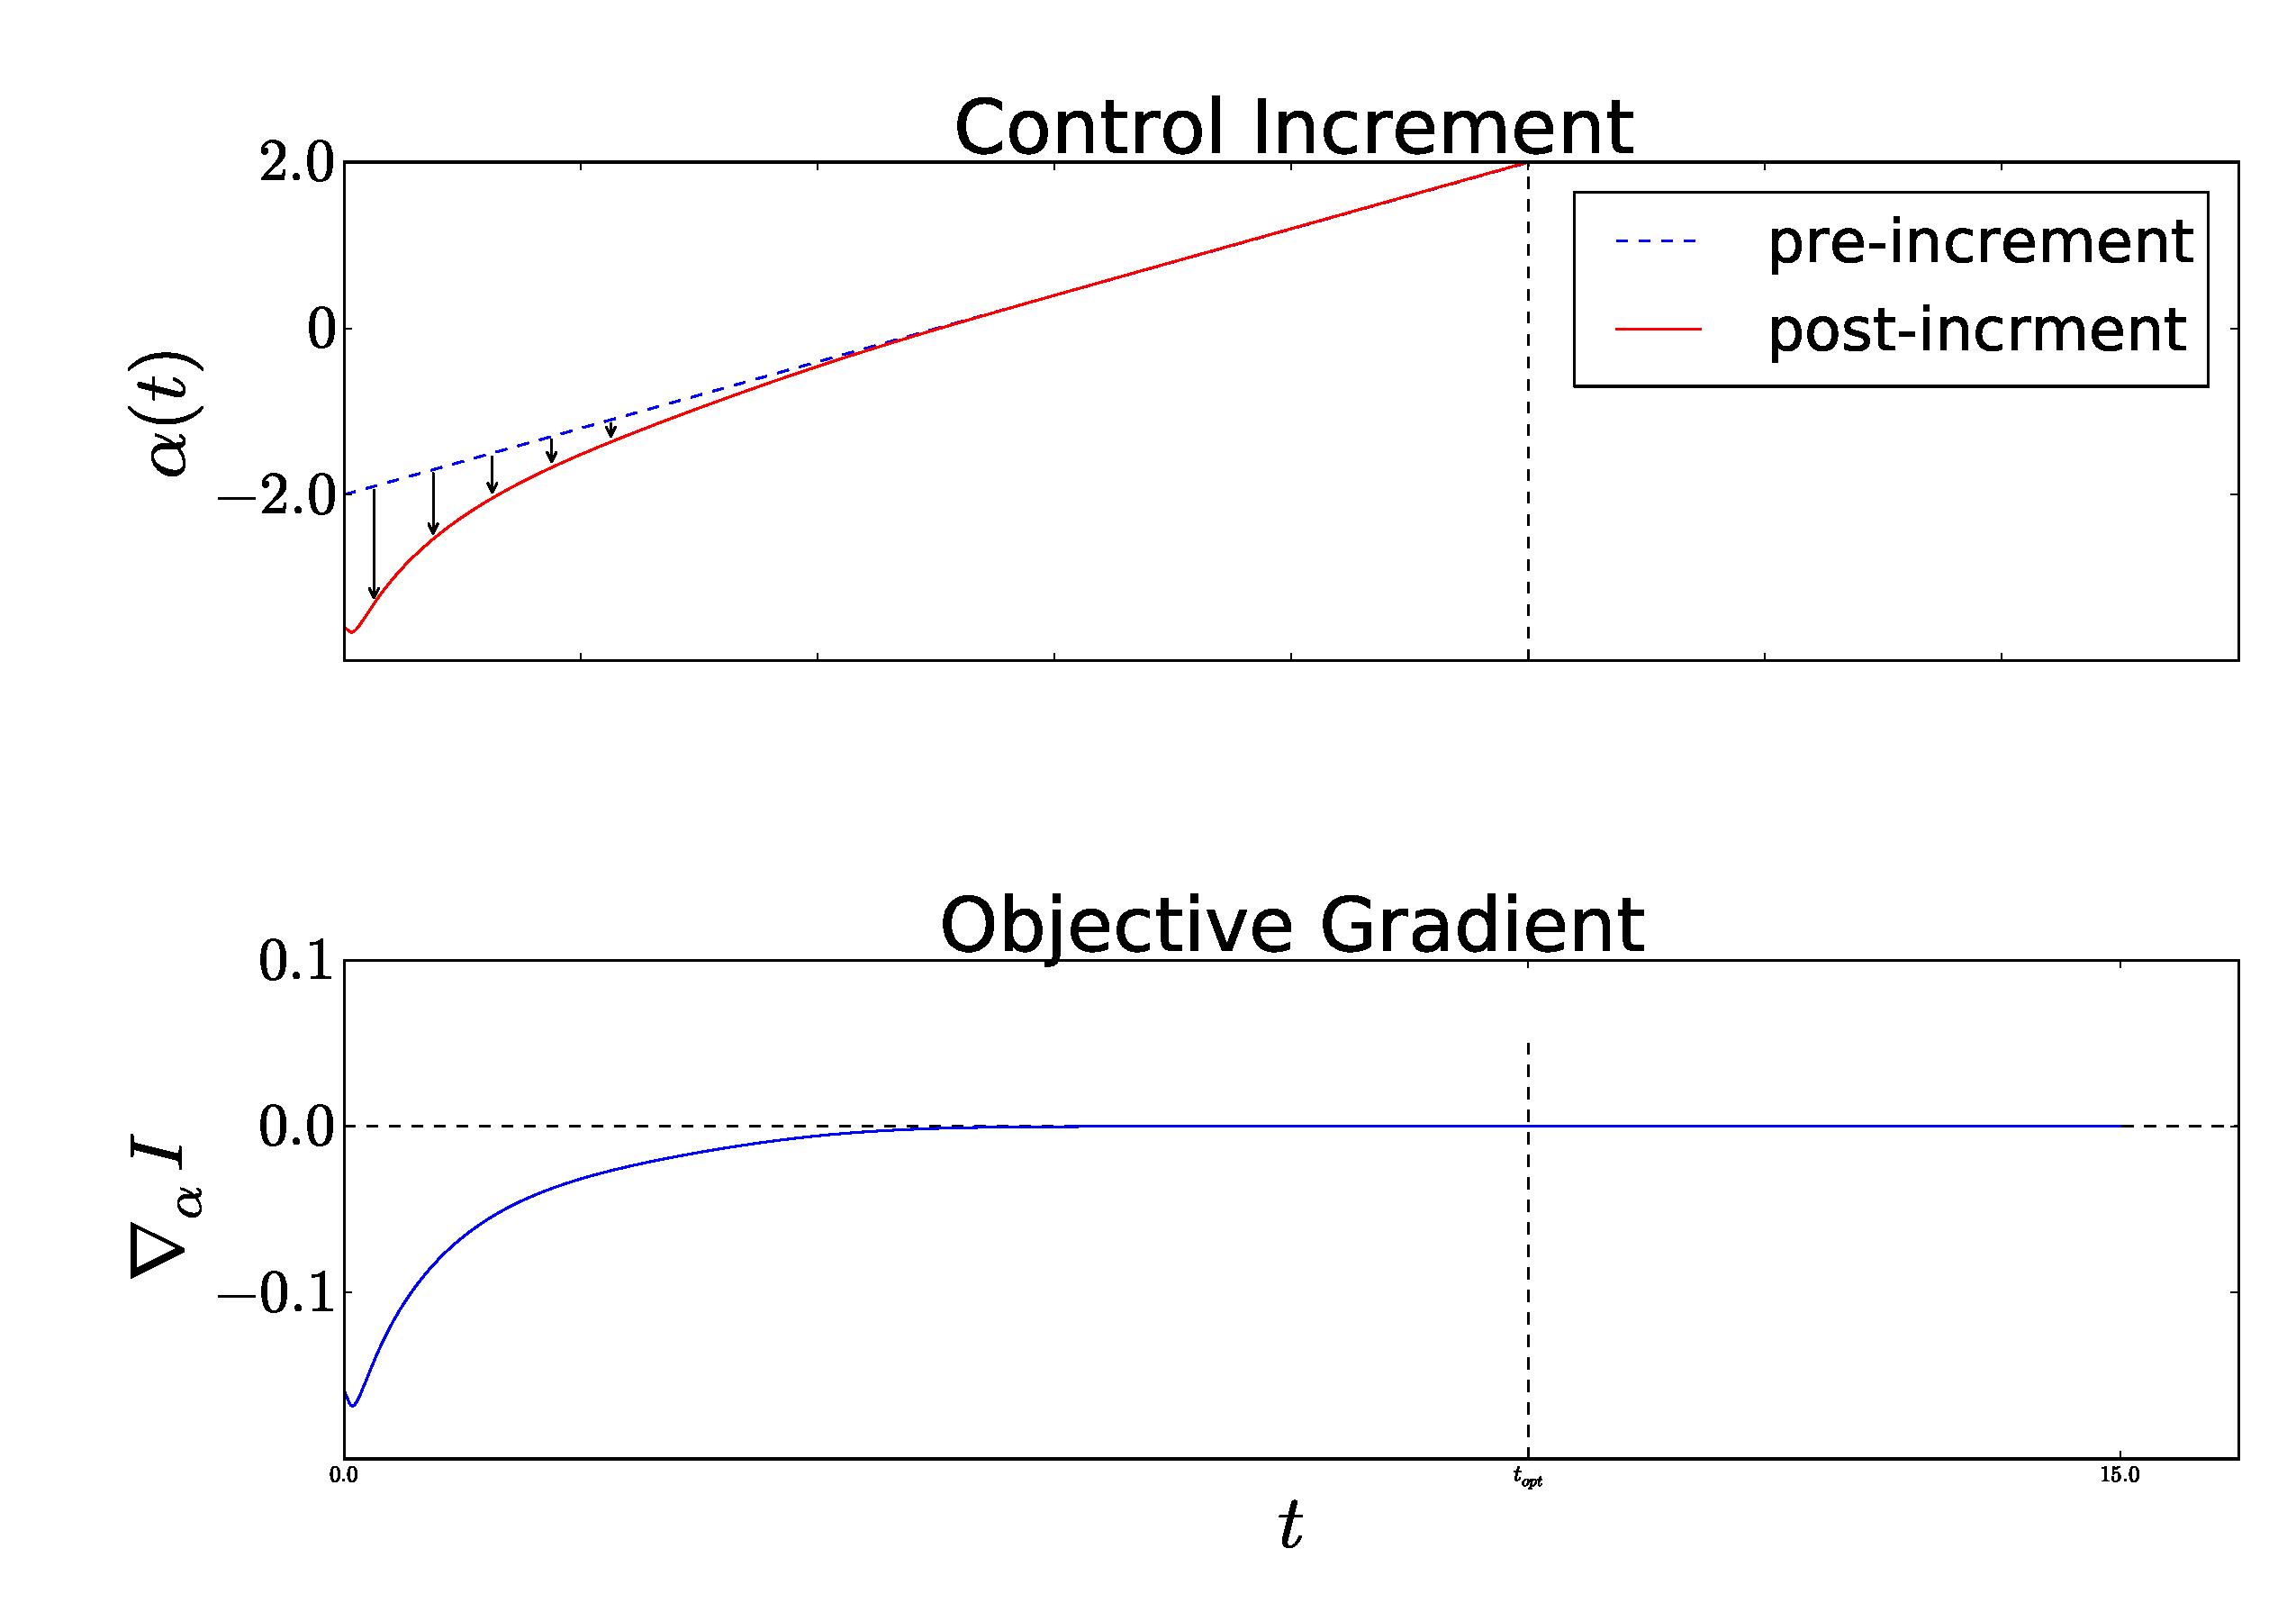
\includegraphics[width=0.8\textwidth]{Figs/FP_Adjoint/control_increment_example.pdf}
  \caption[Single control-increment illustration]{Illustration of how the
  control is incremented given the gradient. Top panel: the
  initial control in dashed and the incremented control in solid with arrows
  indicating the incremental change. Bottom panel: the
  corresponding value of $\delta I/ \delta \a (t)$.
  Note that we only optimize $\a(t)$ for $t \in [0, t_{opt}]$ and set $\a=\amax$
  for $t \in [t_{opt}, t_f]$. Also note that the post-increment $\alpha$ exceeds
  the admissible bounds (here, $[-2,2]$) for some $t$. In practice, for those
  $t$, the post-increment $\a$ will be reset to the closest value within the
  admissible bounds.}
  \label{fig:example_control_increment}    
\end{center}
\end{figure}
           
\begin{figure}[htp] 
\begin{center}
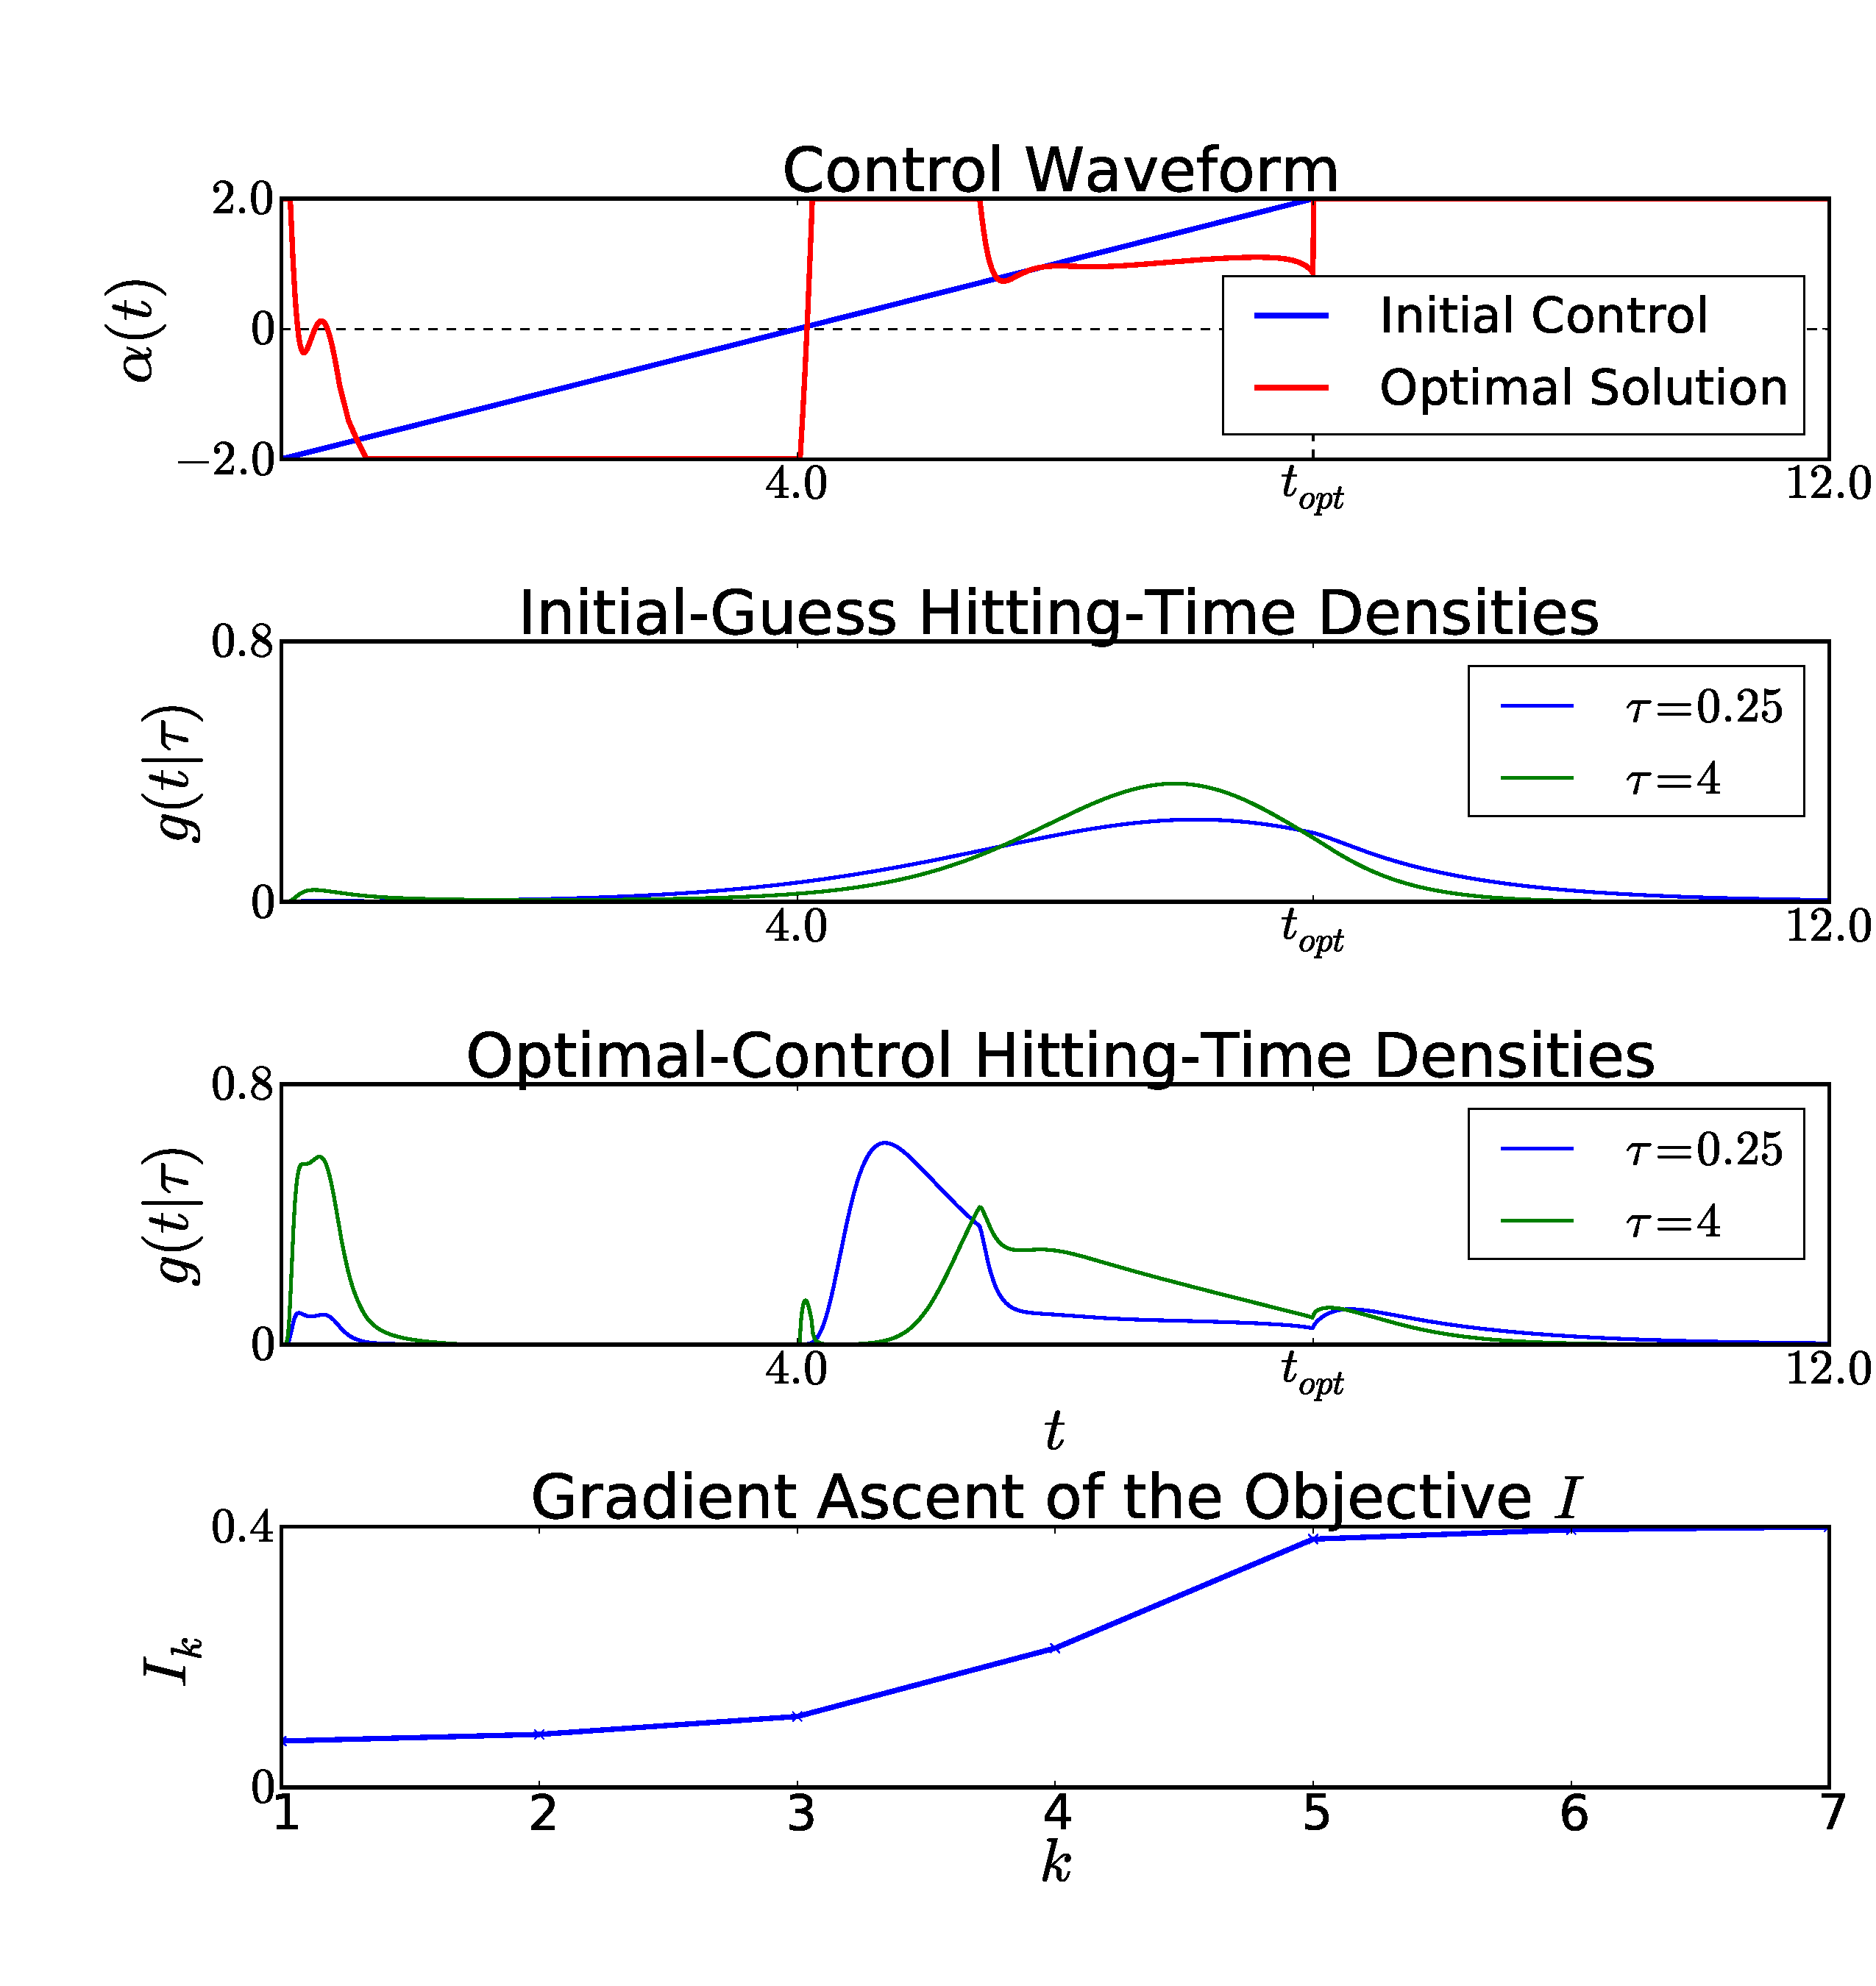
\includegraphics[width=0.95\textwidth]{Figs/AdjointOptimizer/GradientAscent_Nt2.pdf}
\caption[Gradient Ascent for the Optimal Stimulation]{Example of the
    gradient ascent algorithm for the optimization of $I$ in
  \cref{eq:I_mutual_info_objective_in_terms_of_dixf} illustrating that the
  effect of the optimal control is to separate the
  hitting time distributions corresponding to the potential values of
  $\tc$, here for two values of $\tc$.
  Top
  panel: initial and optimal controls, $\a_{0}(t)$ and
  $\a_{opt}(t)$. Second panel: hitting time distributions $g(t|\tc)$ 
  conditional on 
  using the initial control, $\a_0$.
  Third panel: $g(t|\tc)$ conditional on using the
  optimal control, $\a_{opt}$.
 Bottom panel: progress of the mutual information,  
  \cref{eq:J_mutual_info_objective}, as a function of the gradient ascent
  iterations (here the algorithm converged in 9 iterations). The
  optimal control significantly improves the objective in comparison
  to the 
  initial guess.}
  \label{fig:example_gradient_ascent}   
\end{center}   
\end{figure}    
 
\

\subsection{Switch point sweep}
Given the optimal solution obtained in \cref{fig:example_gradient_ascent}, we suspect
that the optimal solution is bang-bang, in the sense of first holding everything back
and then excite maximally. It is interesting to check how sensitive the
objective is to the exact value of the switching time, $t_{switch}$. If it is
not very sensitive, it would be practically useful as the exact
optimization of the PDE-based optimization will not be
necessary, and any bang-bang solution will achieve satisfactory
improvement in the estimation. 
We therefore sweep through different points of exactly when the
bang-bang switch occurs and see how it impacts the resulting objective, $I$.
The results are in \cref{fig:sweep_switchtime}. It seems that, at least for this
parameter set, there is an improvement in the objective by putting the switching
point past $t=6$, but going much beyond that there is no real
difference. 

\begin{figure}[htp]
\begin{center}
  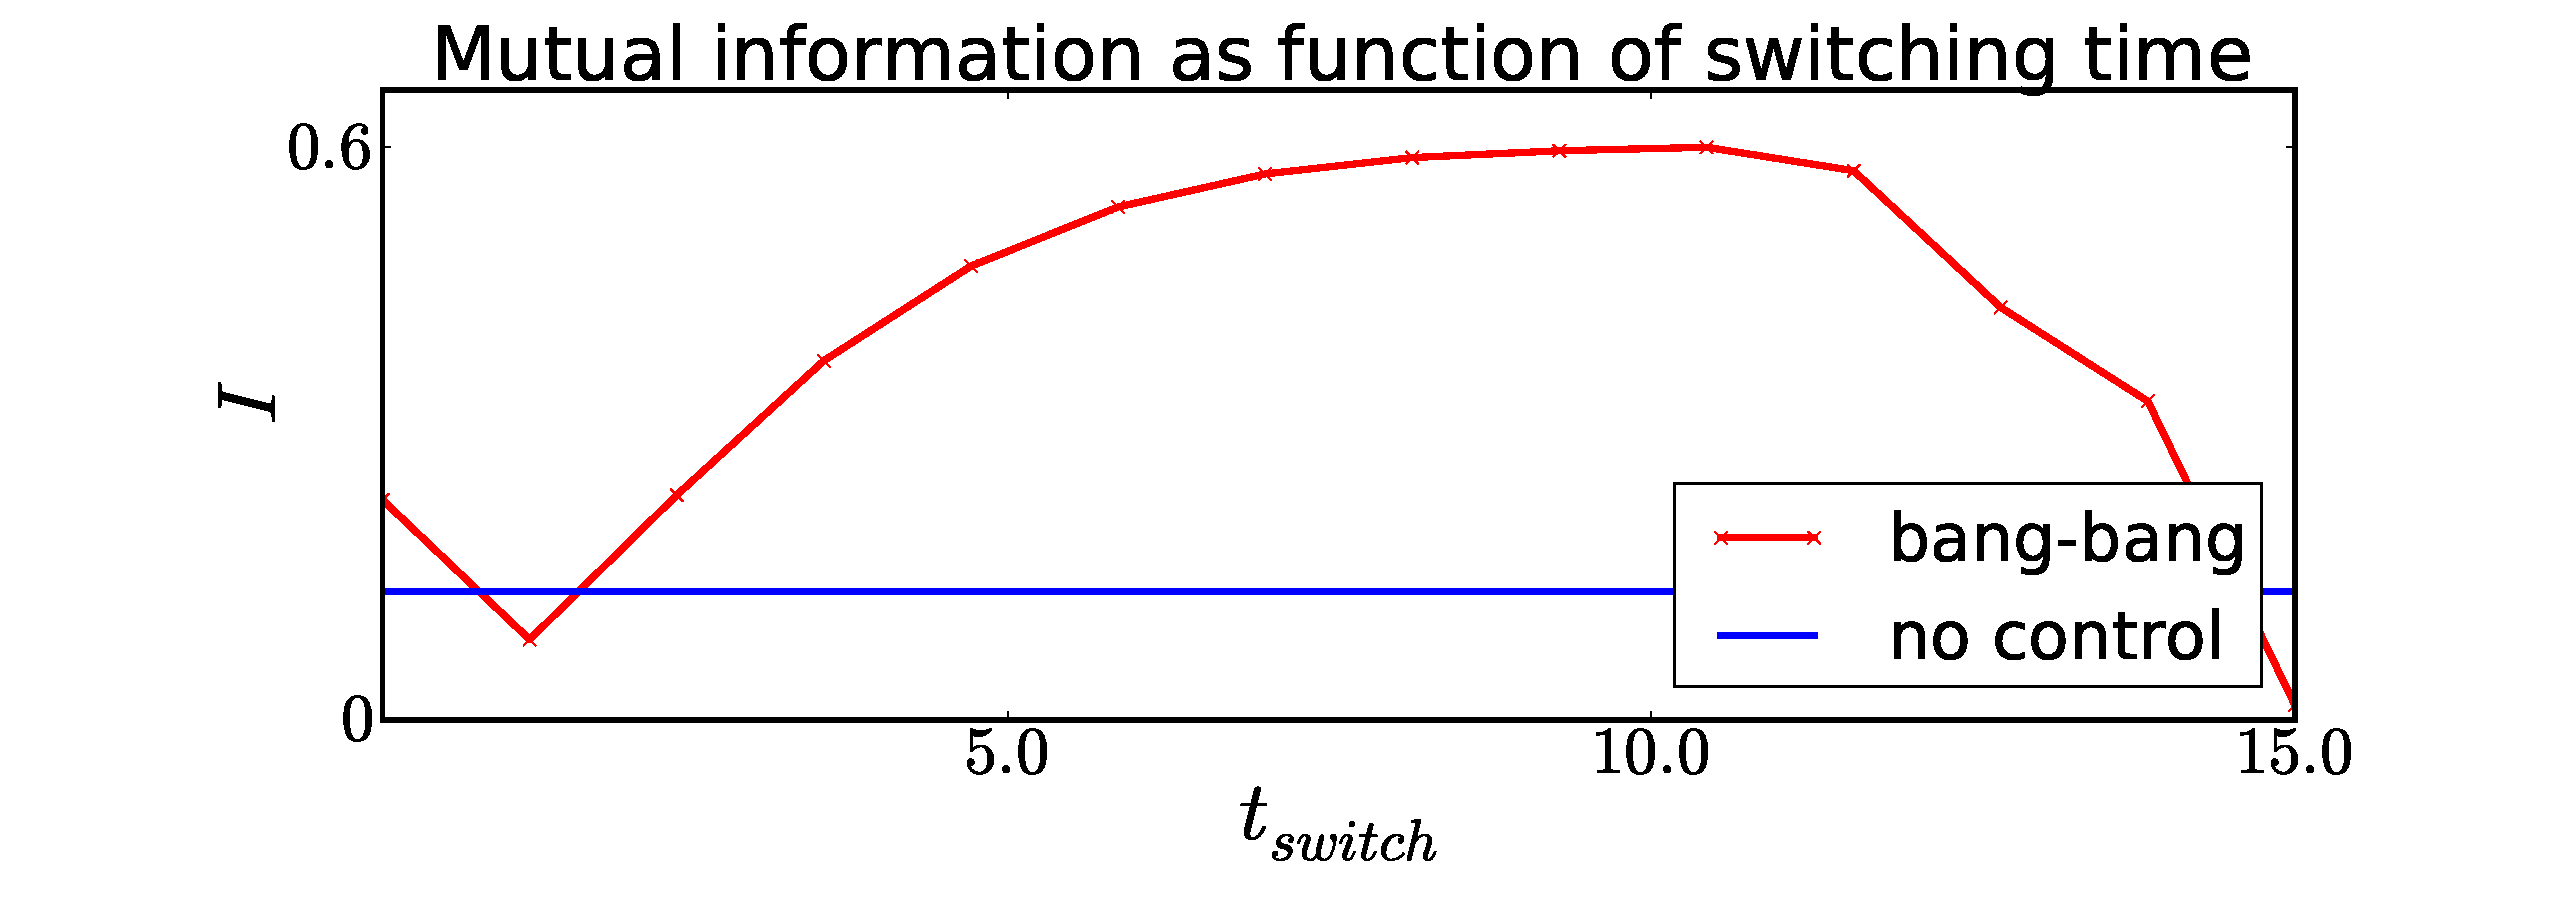
\includegraphics[width=0.8\textwidth]{Figs/AdjointOptimizer/SweepSwitchpoint_wide.pdf}
  \caption[Effect of Switching time on Mutual Info Objective]{Effect of
  switching time in a bang-bang control on the mutual information. The
  red line is the value of the mutual information as a function of the switching
  time between maximally-inhibitive to maximally-excitatory control (a bang-bang
  control). The blue line, plotted for reference, is the value of the
  mutual information for no control ($\a=0$ for all $t$). The same
  simulation parameters are used as in \cref{fig:example_gradient_ascent}. }
  \label{fig:sweep_switchtime}
\end{center}
\end{figure}

\

\subsection{Sensitivity of the Optimization Method} 
In this Section, we explore the effect of the number of points
in the prior; the variance of the prior; the initial
guess for the control $\a(\cdot)$; and the values of the known
parameters $\m$ and $\s$. 

\

\paragraph{Number of points and shape of the prior.} 
It is of interest to know whether the exact shape of the prior matters or whether the first two
moments (mean and variance) are sufficient to determine the optimal control. We
make a simple experiment where we compute the optimal control for two
similar priors, the first using 2 points 
in the prior and the second using 3 points, but the priors have the same
log-mean and log-variance. Results are presented in
\cref{fig:prior_shape_impact}, where it is seen that
the optimal control is essentially the same. This suggests that for practical
purposes it suffices to make the optimization with a 2-point prior that matches
the (log-) variance of the more detailed prior distribution. This
reduces substantially the computational burden.



%\usepackage{graphics} is needed for \includegraphics
\begin{figure}[htp]
\begin{center}
  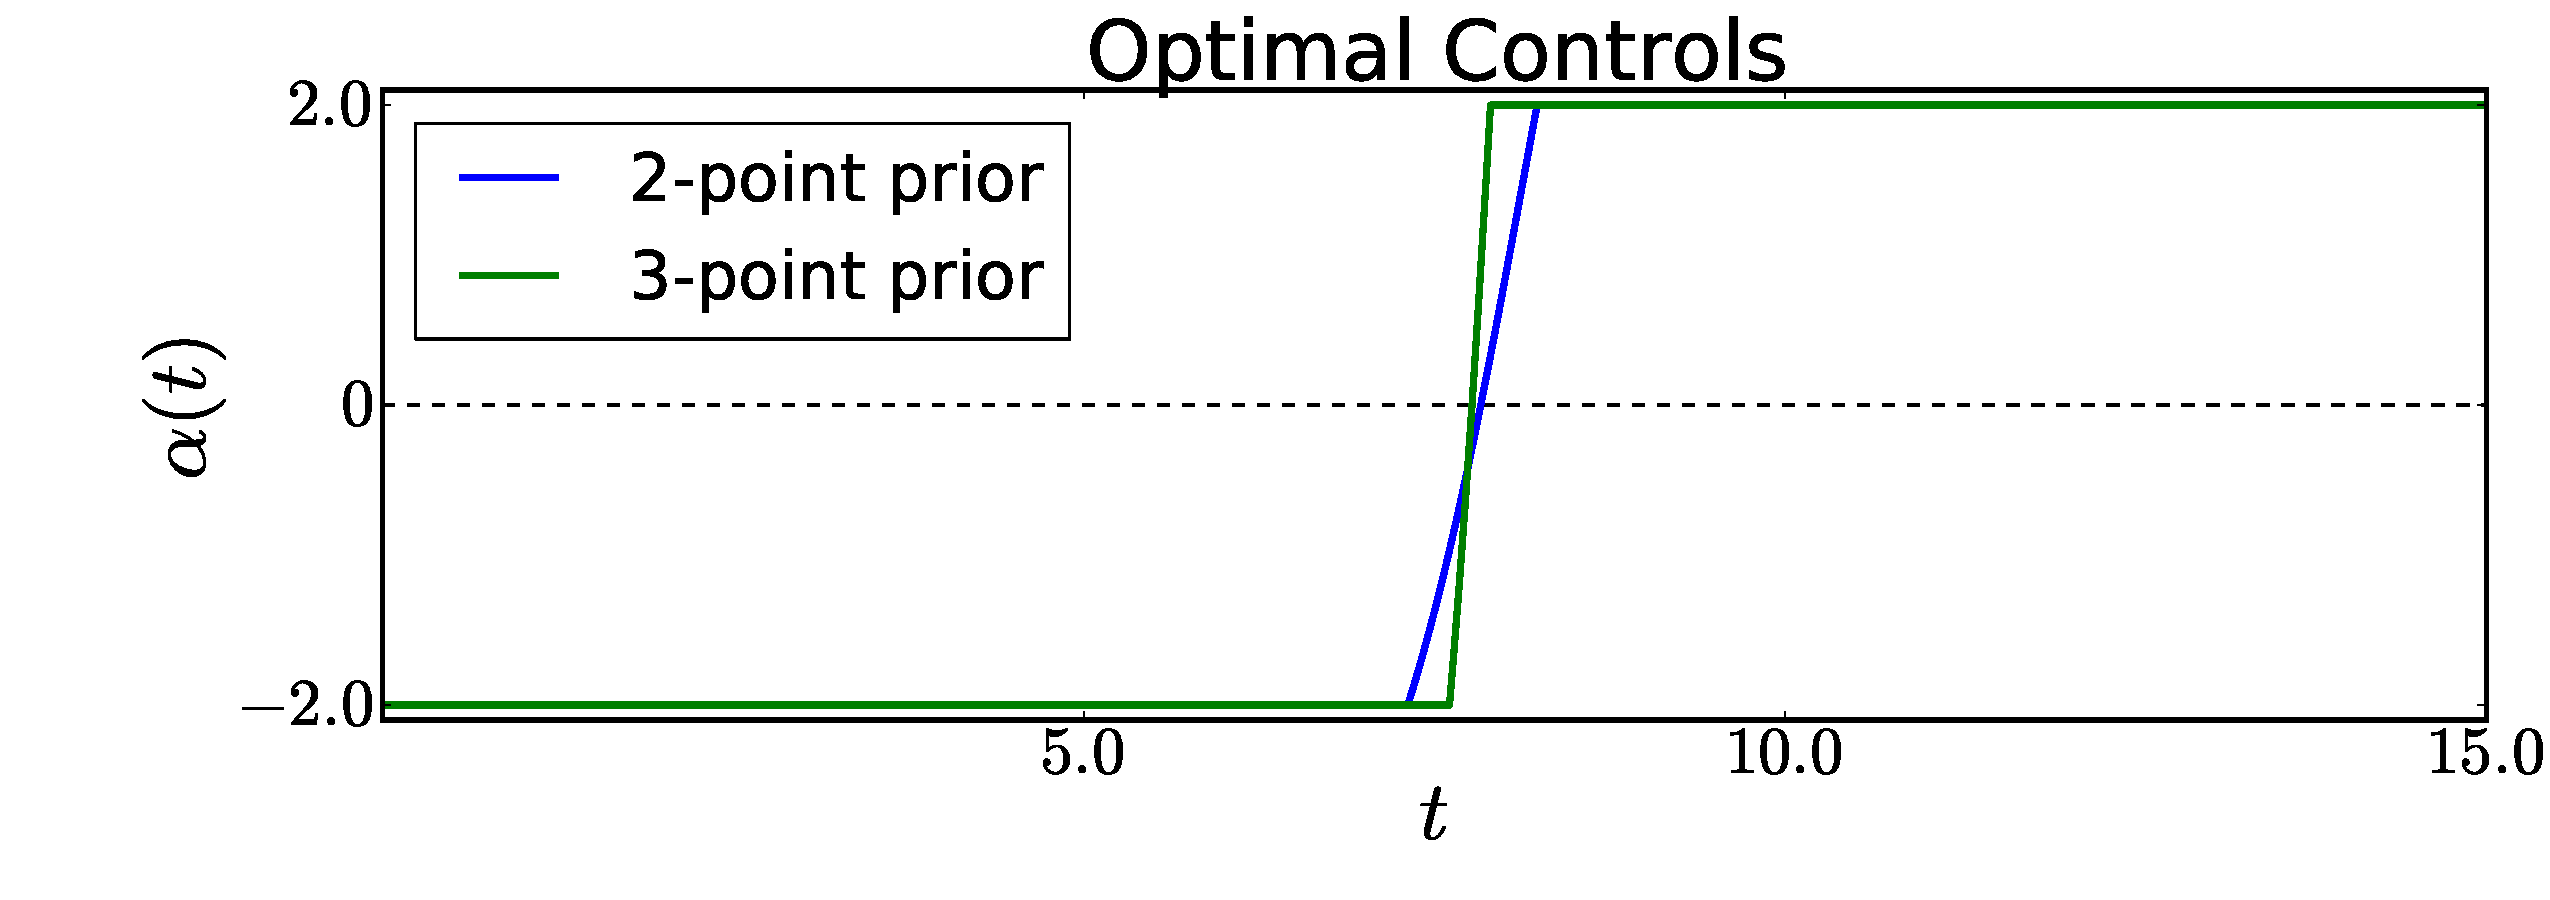
\includegraphics[width=0.8\textwidth]{Figs/AdjointOptimizer/NumberOfTausEffect.pdf}
  \caption[Effect of number of points in prior on Optimal Control]{Effect of the
  number of points in the prior on the Optimal Control. The blue curve was calculated with a 2-points prior, the
  green curve with a 3-points prior. The priors had the same log-mean and log-variance. } 
  \label{fig:prior_shape_impact}
\end{center}
\end{figure}

\

\paragraph{The dispersion of the prior.}
It is also of
interest to know how the dispersion of the prior, here quantified
by the log-variance, changes the optimal control. Again, we take two
2-point priors, one with 
particles at $\tc \in \{1/4, 4\}$ and the other at $\tc \in
\{3/4,4/3\}$. Results
are shown in \cref{fig:prior_dispersion_impact}. It is clear that while the
general shape of the optimal control is the same, regardless of the width of
the prior, there is some difference. We further investigate the
practical difference between the two priors in 
\cref{sec:batch_estimation}.
 
%\usepackage{graphics} is needed for \includegraphics
\begin{figure}[htp]
\begin{center}
  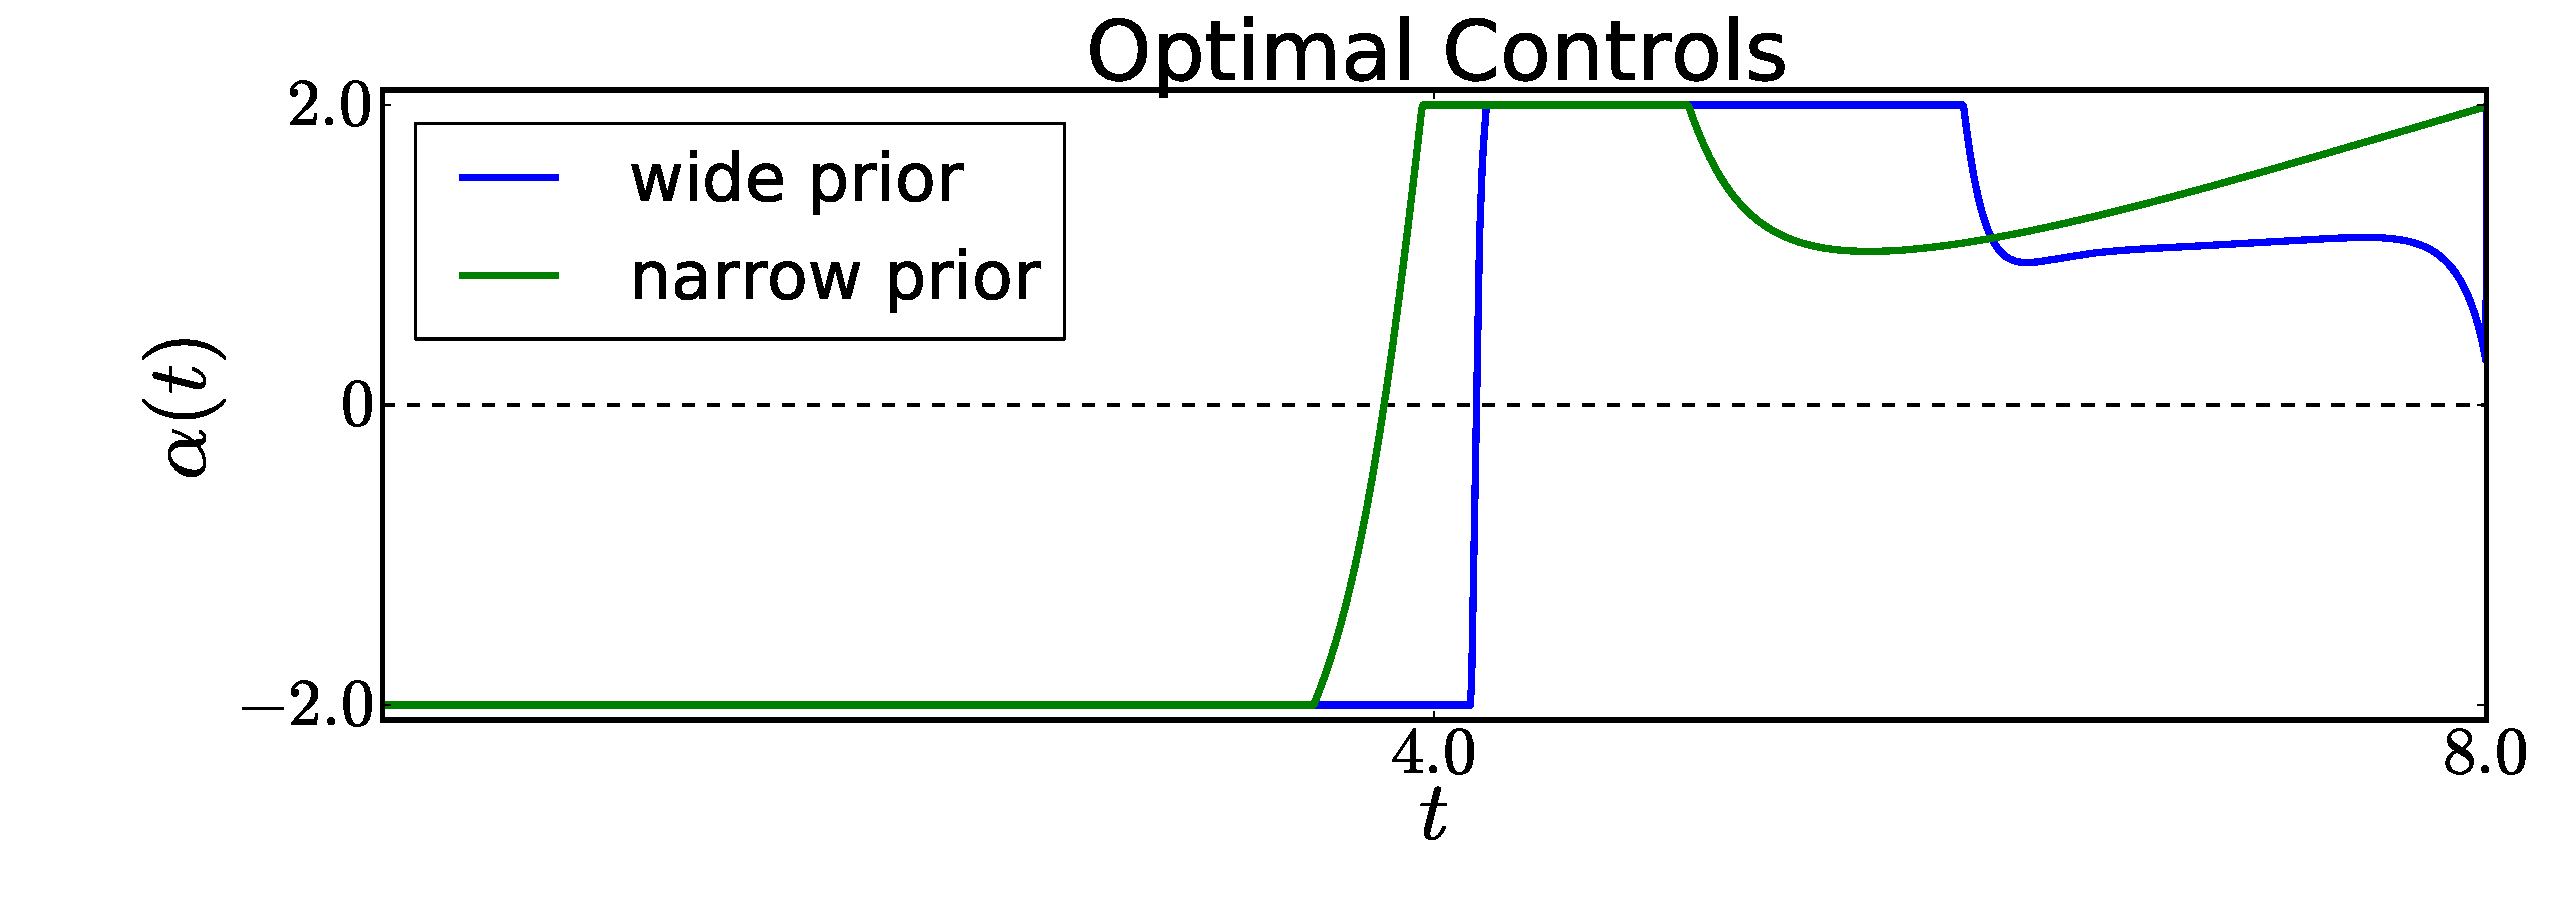
\includegraphics[width=0.8\textwidth]{Figs/AdjointOptimizer/PriorSpread.pdf}
  \caption[Effect of the variance of a prior on the Optimal Control]{Effect of
  the variance of a 2-point prior on the optimal control. The wide prior has probability one half on the values $\tc =  1/4$
  and $4$, while the narrow prior has points positioned much
   closer to each other, $\tc =   3/4$ or $4/3$.  }
  \label{fig:prior_dispersion_impact} 
\end{center}
\end{figure}

\

\paragraph{The initial guess for the control $\a_0$.}

Like all gradient-based optimization procedures, the algorithm is sensitive to the choice
of initial guess for the independent variable, i.e., the choice of
$\a_0$. We illustrate this in \cref{fig:ICs_for_control}. For three
different priors, a wide, a medium and a narrow prior, we run the
optimization scheme from four different initial guesses for 
$\a_0$:

1. zero for the entire (optimization) time interval

2. linearly increasing from the lower to the upper control bound over the
optimization interval

3. a sinusoidal wave from maximum to minimum and again to maximum

4. maximum for the entire optimization time interval 

In \cref{fig:ICs_for_control}, we see that for different initial guesses the
optimization routine finds different optimal controls (see middle panels).  An
initial guess which is non-constant, here linearly increasing or
sinusoidal, are better than the constant initial guesses (the mutual
information is larger, see lower panels). It is also
seen that the shape of the prior does not have much influence on the found
optimal control (the optimal solutions for the same initial guesses but
different priors are close, compare middle panels). The final value of
the mutual information is larger 
for a wider prior (see lower panels), but this is a scaling issue, since of course the
final parameter estimation will be the same if the control is the
same. To summarize: the initial guess of the control is important, and
different initial guesses should be tried to see if the objective can
be improved, whereas the choice of prior distribution is less
important.  

\begin{figure}[h]
\begin{center}
\subfloat[Wide prior]
{
\label{fig:wide_prior_opt_ics}
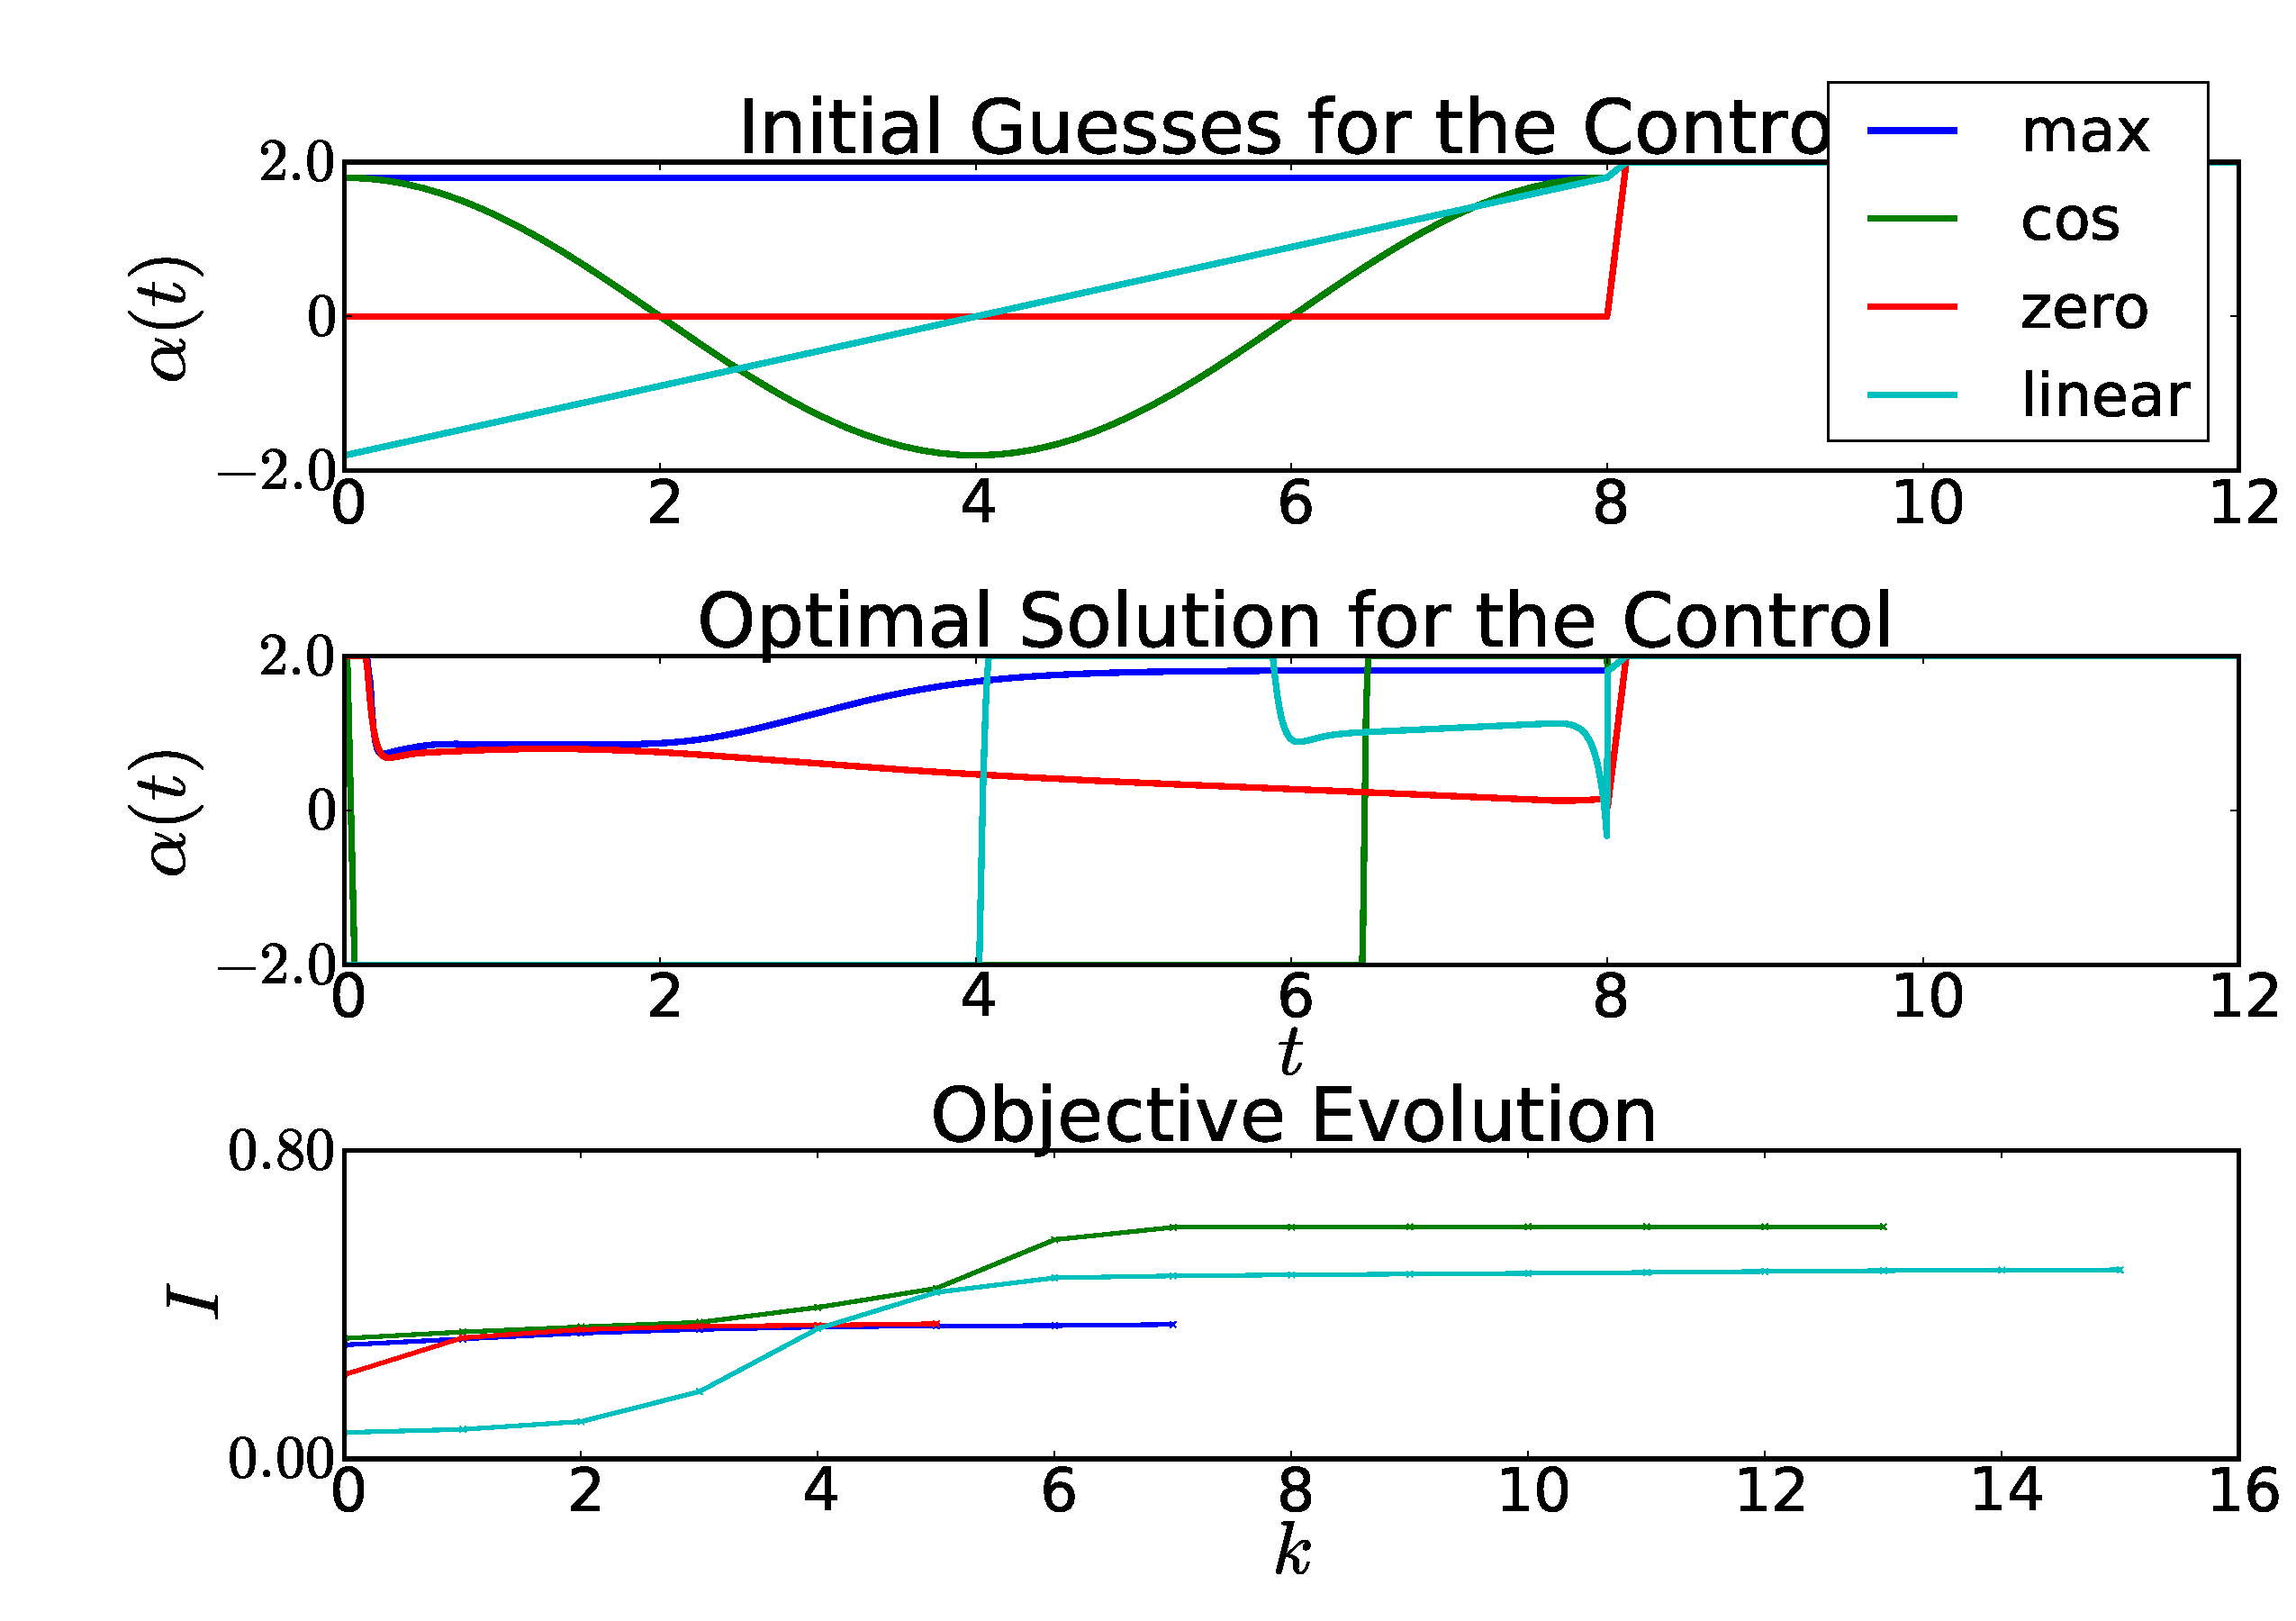
\includegraphics[width=0.5\textwidth]
{Figs/AdjointOptimizer/OptimizerICswide_prior.pdf}
}
\subfloat[Medium prior]
{
\label{fig:medium_prior_opt_ics}
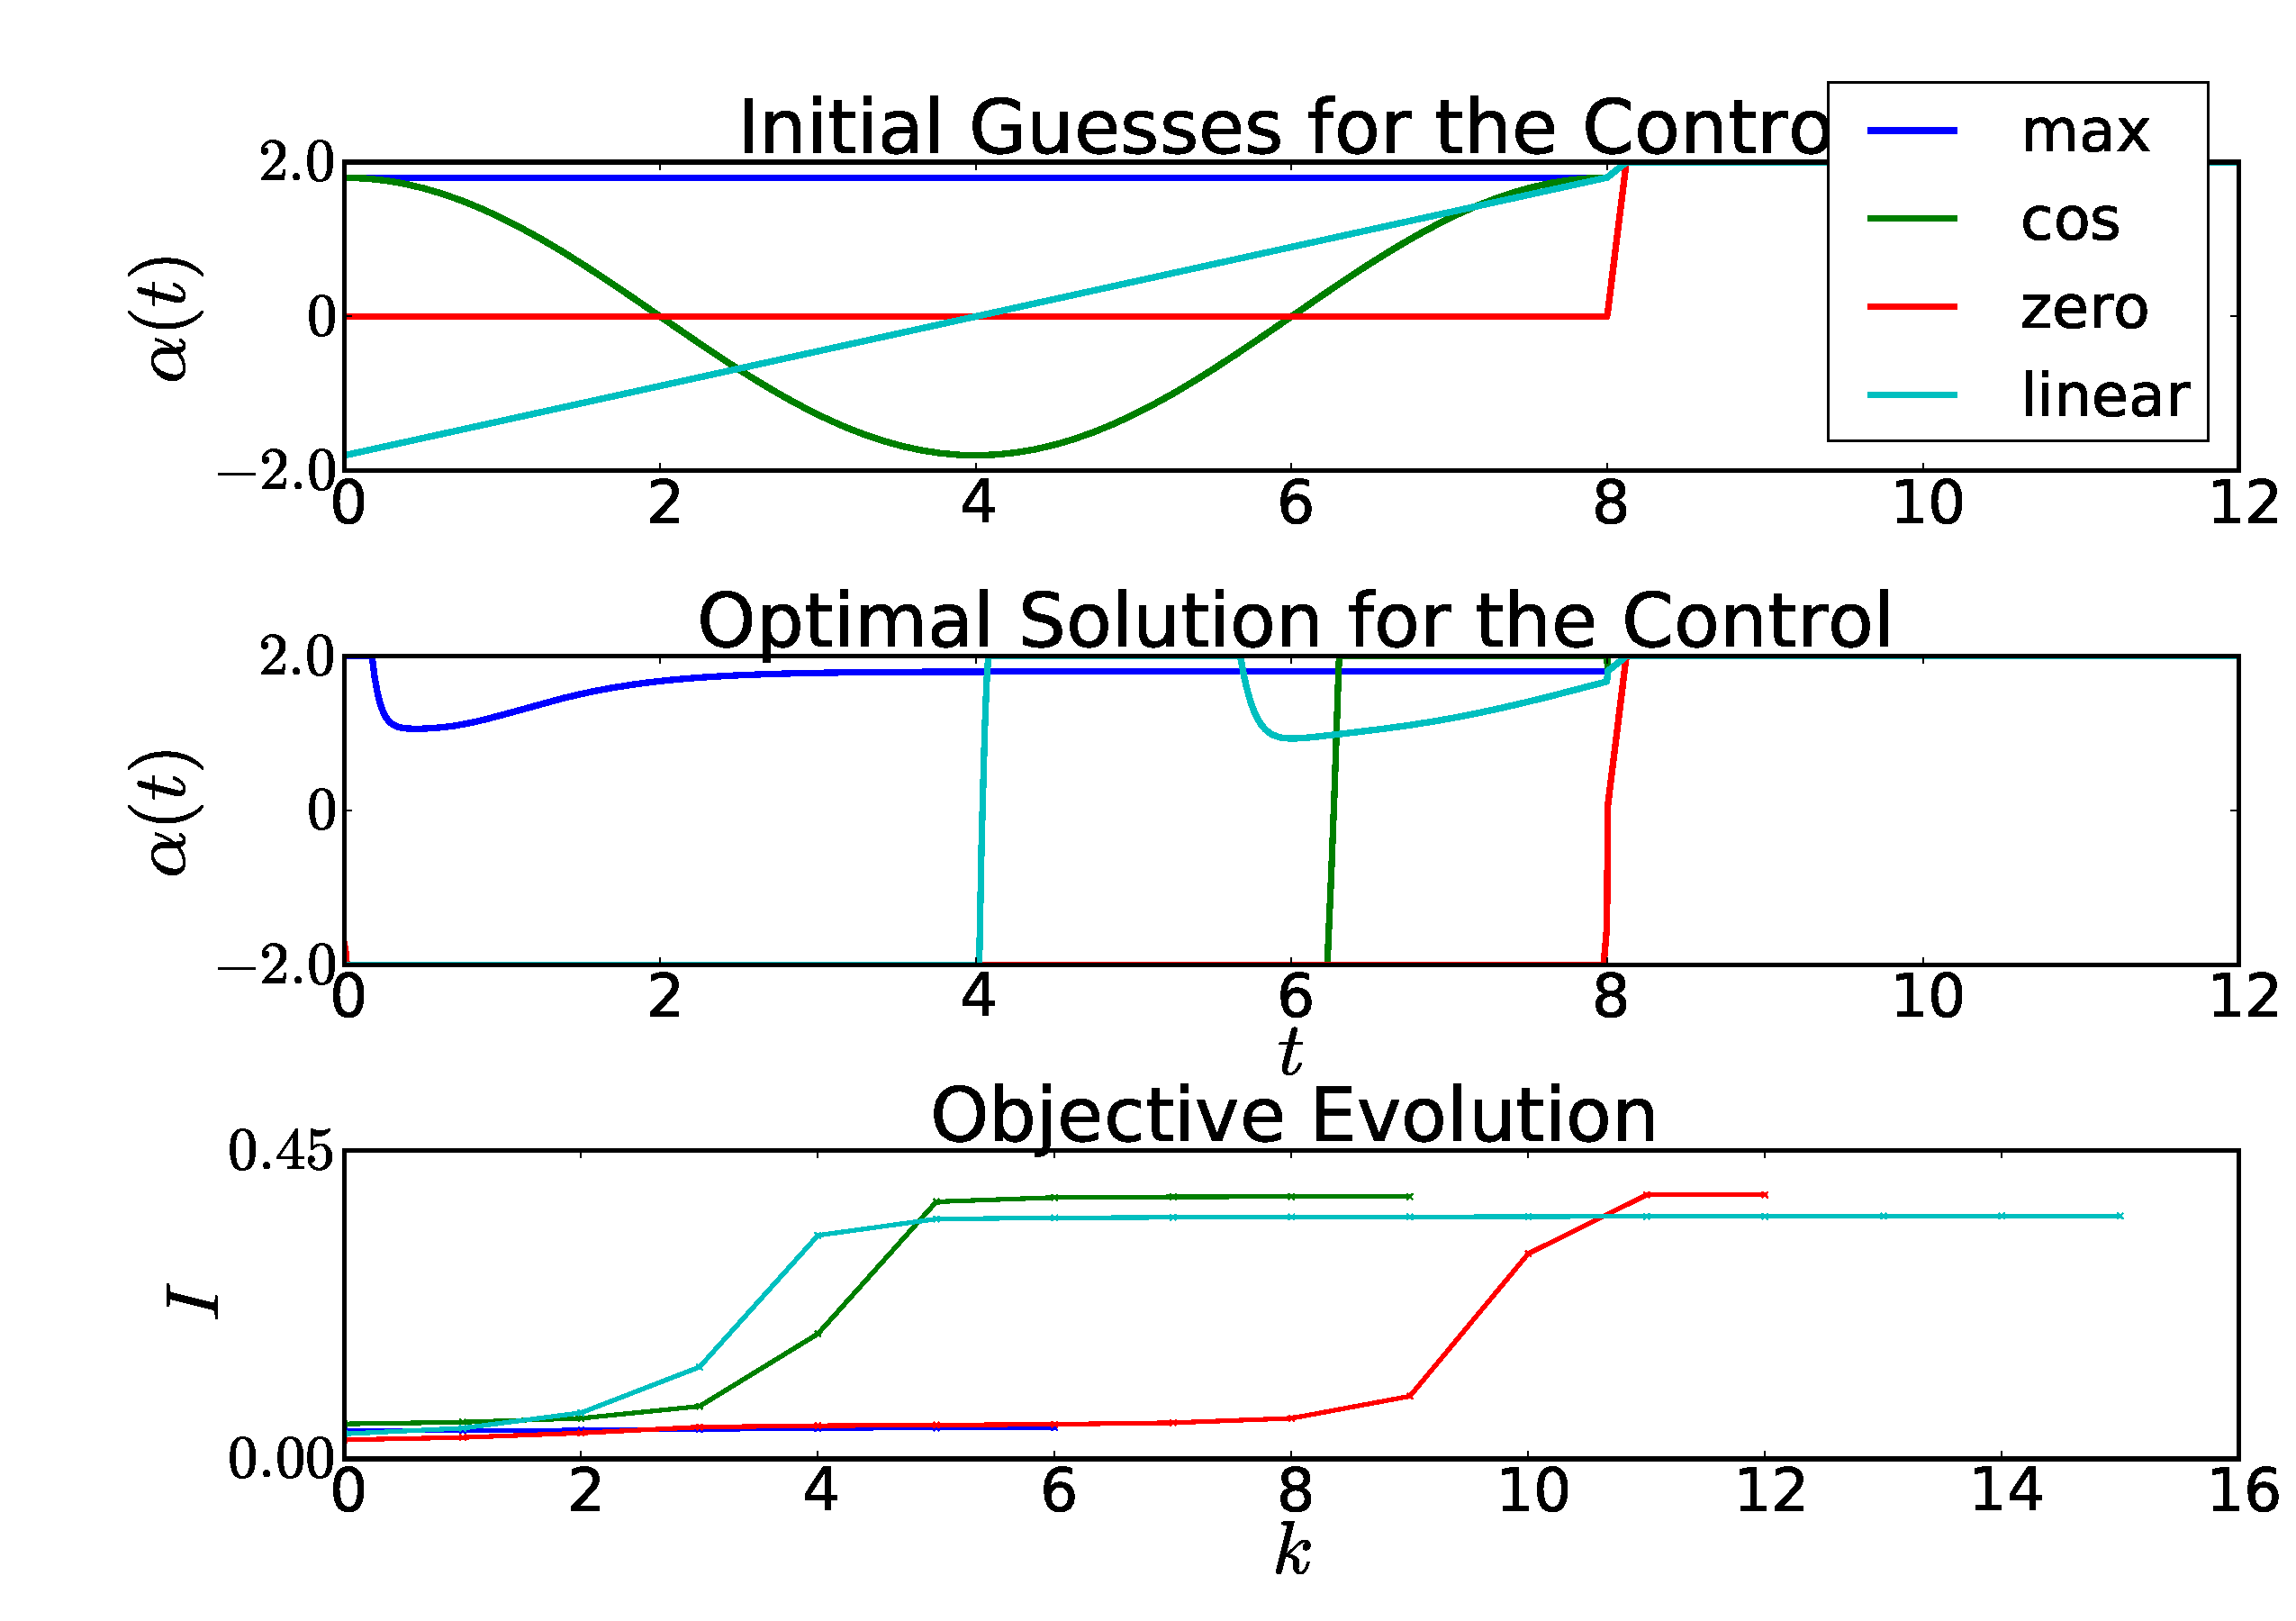
\includegraphics[width=0.5\textwidth]
{Figs/AdjointOptimizer/OptimizerICsmedium_prior.pdf}
}
\\
\subfloat[Narrow prior]
{
\label{fig:medium_prior_opt_ics}
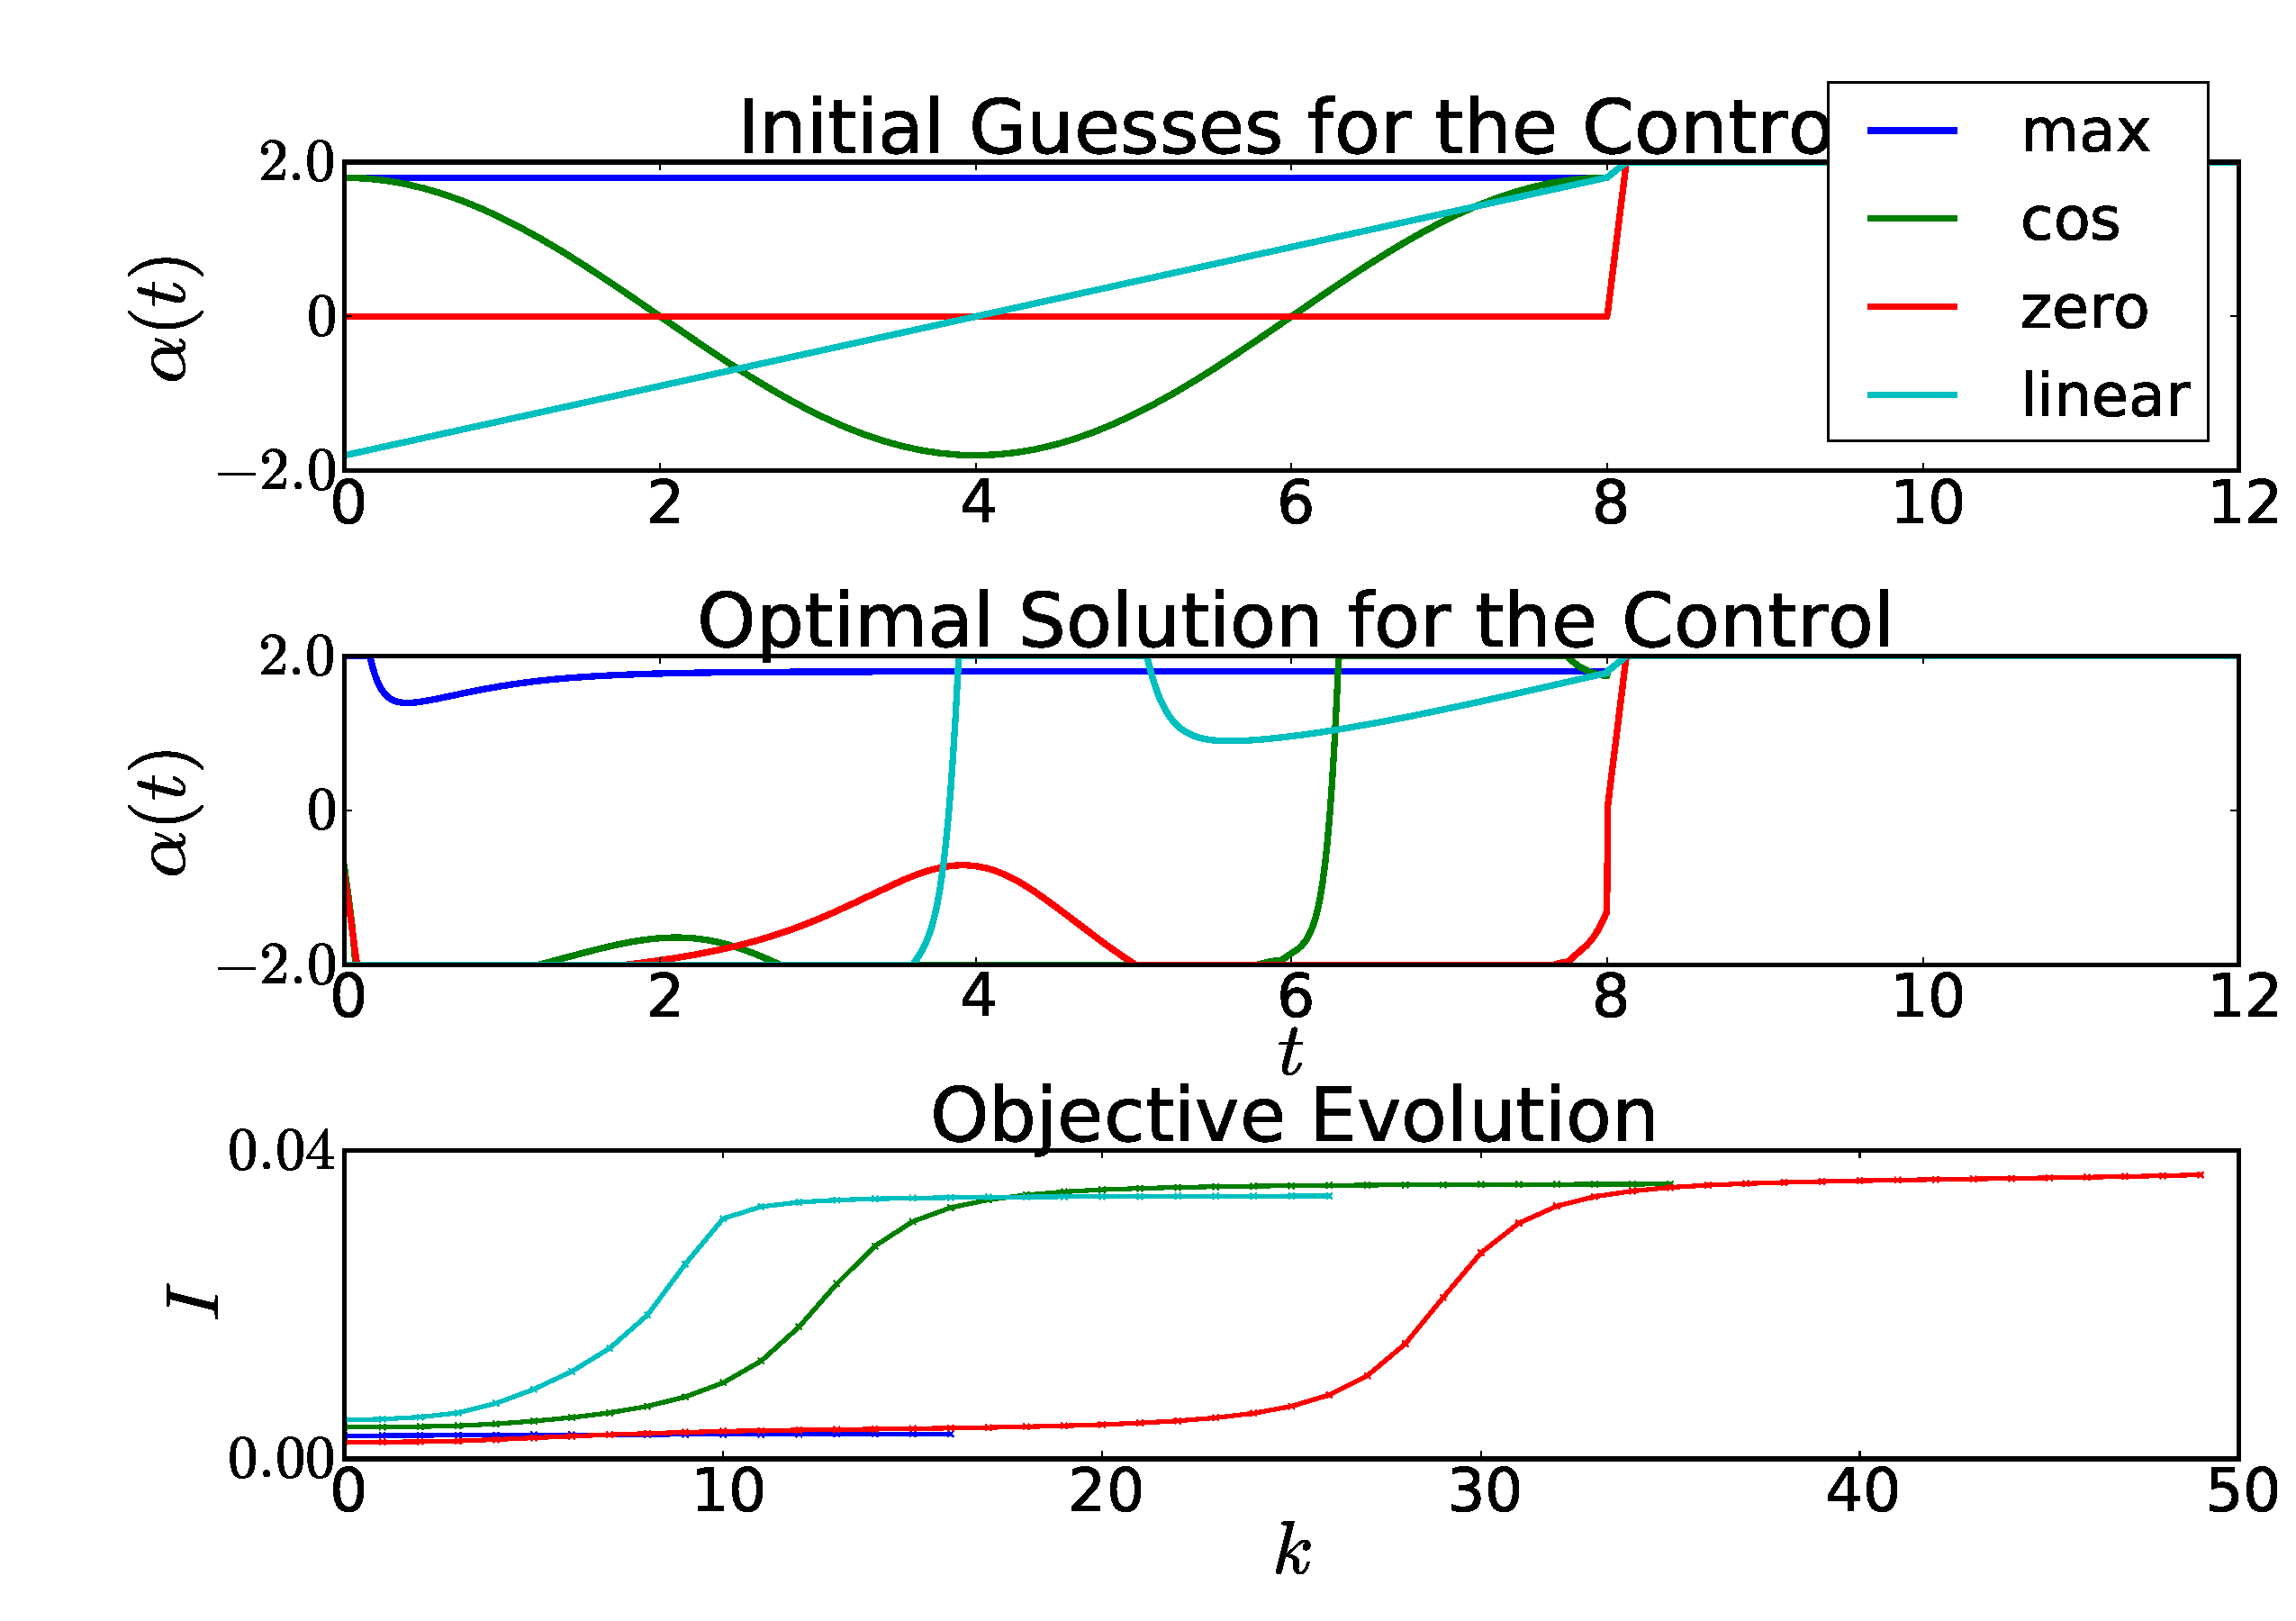
\includegraphics[width=0.5\textwidth]
{Figs/AdjointOptimizer/OptimizerICsconcentrated_prior.pdf}
}
% \subfloat[Labels for initial controls]
% {
% \label{fig:medium_prior_opt_ics}
% \hspace{20mm}\includegraphics[width=0.4\textwidth]
% {Figs/AdjointOptimizer/legend_labels.jpg}\hspace{20mm}
% }
\caption[Dependence on initial guess for control]{Illustration of the dependence
of the optimization scheme on the initial guess for the optimal
control for a wide prior (a), a medium prior (b) and a narrow prior (c). 
In the top panels the initial guesses are shown, in the middle
panels the corresponding solution obtained by the optimization routine
are shown,
in the bottom panels the corresponding evolutions of the mutual
information are shown.
The various initial conditions considered are: maximum stimulation for all $t$,
(blue); sinusoidal stimulation (green); no control at all, $\a=0$, (red) and a
linearly increasing control from min to max (cyan)}
\label{fig:ICs_for_control}
\end{center}
\end{figure}

\

\paragraph{Values of the known parameters $\mu, \s$.} 
So far we have restricted ourselves to one scenario of the assumed known
parameters, $\mu=0$ and $\s=1$. 
%When no control is applied, this corresponds to the sub-threshold 
%regime, meaning that in absence of noise there would never be a
%spike. If maximally stimulated, i.e., the control equals $\amax$, this
%corresponds to super-threshold, meaning that in absence of noise
%there would be regular spikes.  

% (ALEX: this section, It needs a couple more sentences describing what
% happened.)
We also redid the basic analyses by varying these parameters, analyzing six
qualitatively different sets of parameter values. In all cases the same 2-point
prior was used, with probability one half on $\tc = 1/2$ and $2$. The following
parameter sets were investigated: $(\mu,\s)=(-0.5, 1), (0.1,1)$, $(1,1), (0, 
0.3), (0, 0.9)$ and $(0,1.5)$. In all cases the algorithm succeeded in finding
an optimal control (a different for each pair), that significantly increased the
mutual information relative to that of the initial control guess (results not
shown). Although not an exhaustive study, this strongly suggests that our
optimal design procedure is applicable and would be effective for a wide range
of the values of $\m,\s$.  

\section{Batch Estimation}
\label{sec:batch_estimation}
We now proceed to generate a large sample of hitting times with several types
of controlled stimulation and then estimate the unknown
parameter after observing the whole sample. We call this batch estimation as opposed to
online estimation, where estimates are updated after every single
observation, and where the control is updated according to the updated prior distribution.
Online estimation is performed in \cref{sec:online_estimation}.
 
We assume that the true parameters governing \cref{eq:X_evolution_uo_control}
are as before; $ \m = 0, \tc = 1$ and $ \s = 1$. We will assume $\s, \m$
known and only estimate the time constant $\tc$, so
we will maximize the mutual information between $\ts$ and $\tc$. To
obtain the optimal control, we take a discrete uniform prior on 
 $\tc$, using 10 points uniformly spaced in the interval $[0.25, 4.0]$, i.e.,
 each point in the prior has probability 1/10. Note that neither the mean nor the
 log-mean of the prior correspond to the unknown true $\tc$ or $\log(\tc)$.
 
The obtained control is denoted the "optimal control". In addition, we consider 
two optimal controls obtained using a 'wide' and a 'narrow' 2-point prior, as
shown in \cref{fig:prior_dispersion_impact}. We call these 'opt-wide' for the
prior with $\tc =  [0.25, 4]$, and 'opt-narrow' for the prior with  $\tc =  
[0.75, 1/0.75]$.  

In addition, we also use the control where $\a$ is set to the fixed 'critical' value 
$\a = \a_{crit} = \xth/\tc = 1$, and one where the control is set to its upper
bound, $\a = \amax$. The critical value, $\xth/\tc$, defines the least
value for $\a$ such that the system can reach the spiking threshold in the
absence of noise (i.e.\ if $\s=0$).
% (ALEX: explain in what sense or why the first case is a
% 'critical' value)

\subsection{The Estimation Algorithm for the Batch Problem}

We have posed a fairly-simple estimation objective, namely to estimate $\tau$, which
amounts to single-variable optimization. The negative log-likelihood of an
observed hitting-time set $\{t_n\}$ is
\begin{equation}
l(\tc) = - \sum_n \log ( g(t_n | \tc) ) =  - \sum_n \log ( -\frac{\s^2}2 \di_x
f(t_n | \tc) |_{\xth} ).
\label{eq:MLE_likelihood}
\end{equation}
We minimize \cref{eq:MLE_likelihood} using the standard single-variable
optimization routine in NumPy based on Brent's method.

% The distributions are exemplified in
% \cref{fig:log_likelihood_beta_examples_100000},
% for three different values of $N_s =  10^5$. We see that for the constant
% stimulations, $\a = \a_{crit}, \a_{max}$ it is very hard to
% distinguish between different values of $\tc$. 
% 
% In \cref{fig:log_likelihood_beta_examples_100000} as well as in 
% \cref{fig:hitting_time_density_g_aopt_bprior}, we get an indication for why
% the 'optimal control' is better than the constants. For the constant control
% the different hitting time densities look like local perturbations of each
% other, either a little more or a little less, but for the optimal control they
% are shifted, which means that we see the first indications that the Opt Control,
% might have some superiority over the 'Crit' Control (for example) as it seems to estimate a $\tc$ closer to 1 (the 'true' value). However, on average, the different shapes of $\a(t)$ seems to have a very limited impact on the estimates for $\tc$ (even though it has a very obvious impact on the shape of the hitting time distribution $g(t)$).

% \begin{figure}[h] 
% \begin{center}
% \subfloat[opt]
% {
% \includegraphics[width=.75\textwidth]
% {Figs/HitTime_MI_TauChar_Adjoint_Estimate/Adjoint_TauChar_Estimator_estimatorWorkbench_b=0x100000_a0.pdf}
% }
% \\
% \subfloat[crit] 
% {
% \includegraphics[width=.75\textwidth]
% {Figs/HitTime_MI_TauChar_Adjoint_Estimate/Adjoint_TauChar_Estimator_estimatorWorkbench_b=0x100000_a1.pdf}
% }
% \\
% \subfloat[max]
% {
% \includegraphics[width=.75\textwidth]
% {Figs/HitTime_MI_TauChar_Adjoint_Estimate/Adjoint_TauChar_Estimator_estimatorWorkbench_b=0x100000_a2.pdf}
% }
% \caption[labelInTOC]{Example of Empirical vs.\ Analytical Hitting time
% distributions, $g(t|\t;\a)$, and the associated log-likelihoods. $N_s = 10^5$
% hits}
% \label{fig:log_likelihood_beta_examples_100000}
% \end{center}
% \end{figure}  
% 
% \clearpage



\subsection{Comparison of Estimators}

Recall that we will stimulate the system using 5 stimulation
waveforms.  
\begin{enumerate}
  \item 'opt' - the optimal gradient-ascent-based  control $\a_{opt}$, based on
  a 10-point uniform prior between $[0.25, 4]$
  \item  'opt-wide' - the optimal control using a 2-point prior on  $[0.25, 4]$
  \item 'opt-narrow' - the optimal control using a 2-point prior on $[0.75,
  1/0.75]$
\item   'crit' - the constant control
$\a_{crit}$, ($\a_{crit}(t) =  \xth/\tc$
\item  'max' - the max constant control, $\amax$ ($=2$)
\end{enumerate} 

We now simulate $N_b $ blocks of $N_s$ hitting times each for the
5 alphas. We then estimate $\tc$ over each set using Maximum-Likelihood with our
computed expression for the density, $g(t|\tc; \a(t) )$. 
Naturally, for each control, we use the same Gaussian random draws per block of
$N_s$ hitting times. The estimation results are tabulated in 
\cref{tab:beta_estimates_from_hitting_times_different_alphas}.

%\usepackage{graphics} is needed for \includegraphics
% \begin{figure}[htp]
% \begin{center}
%   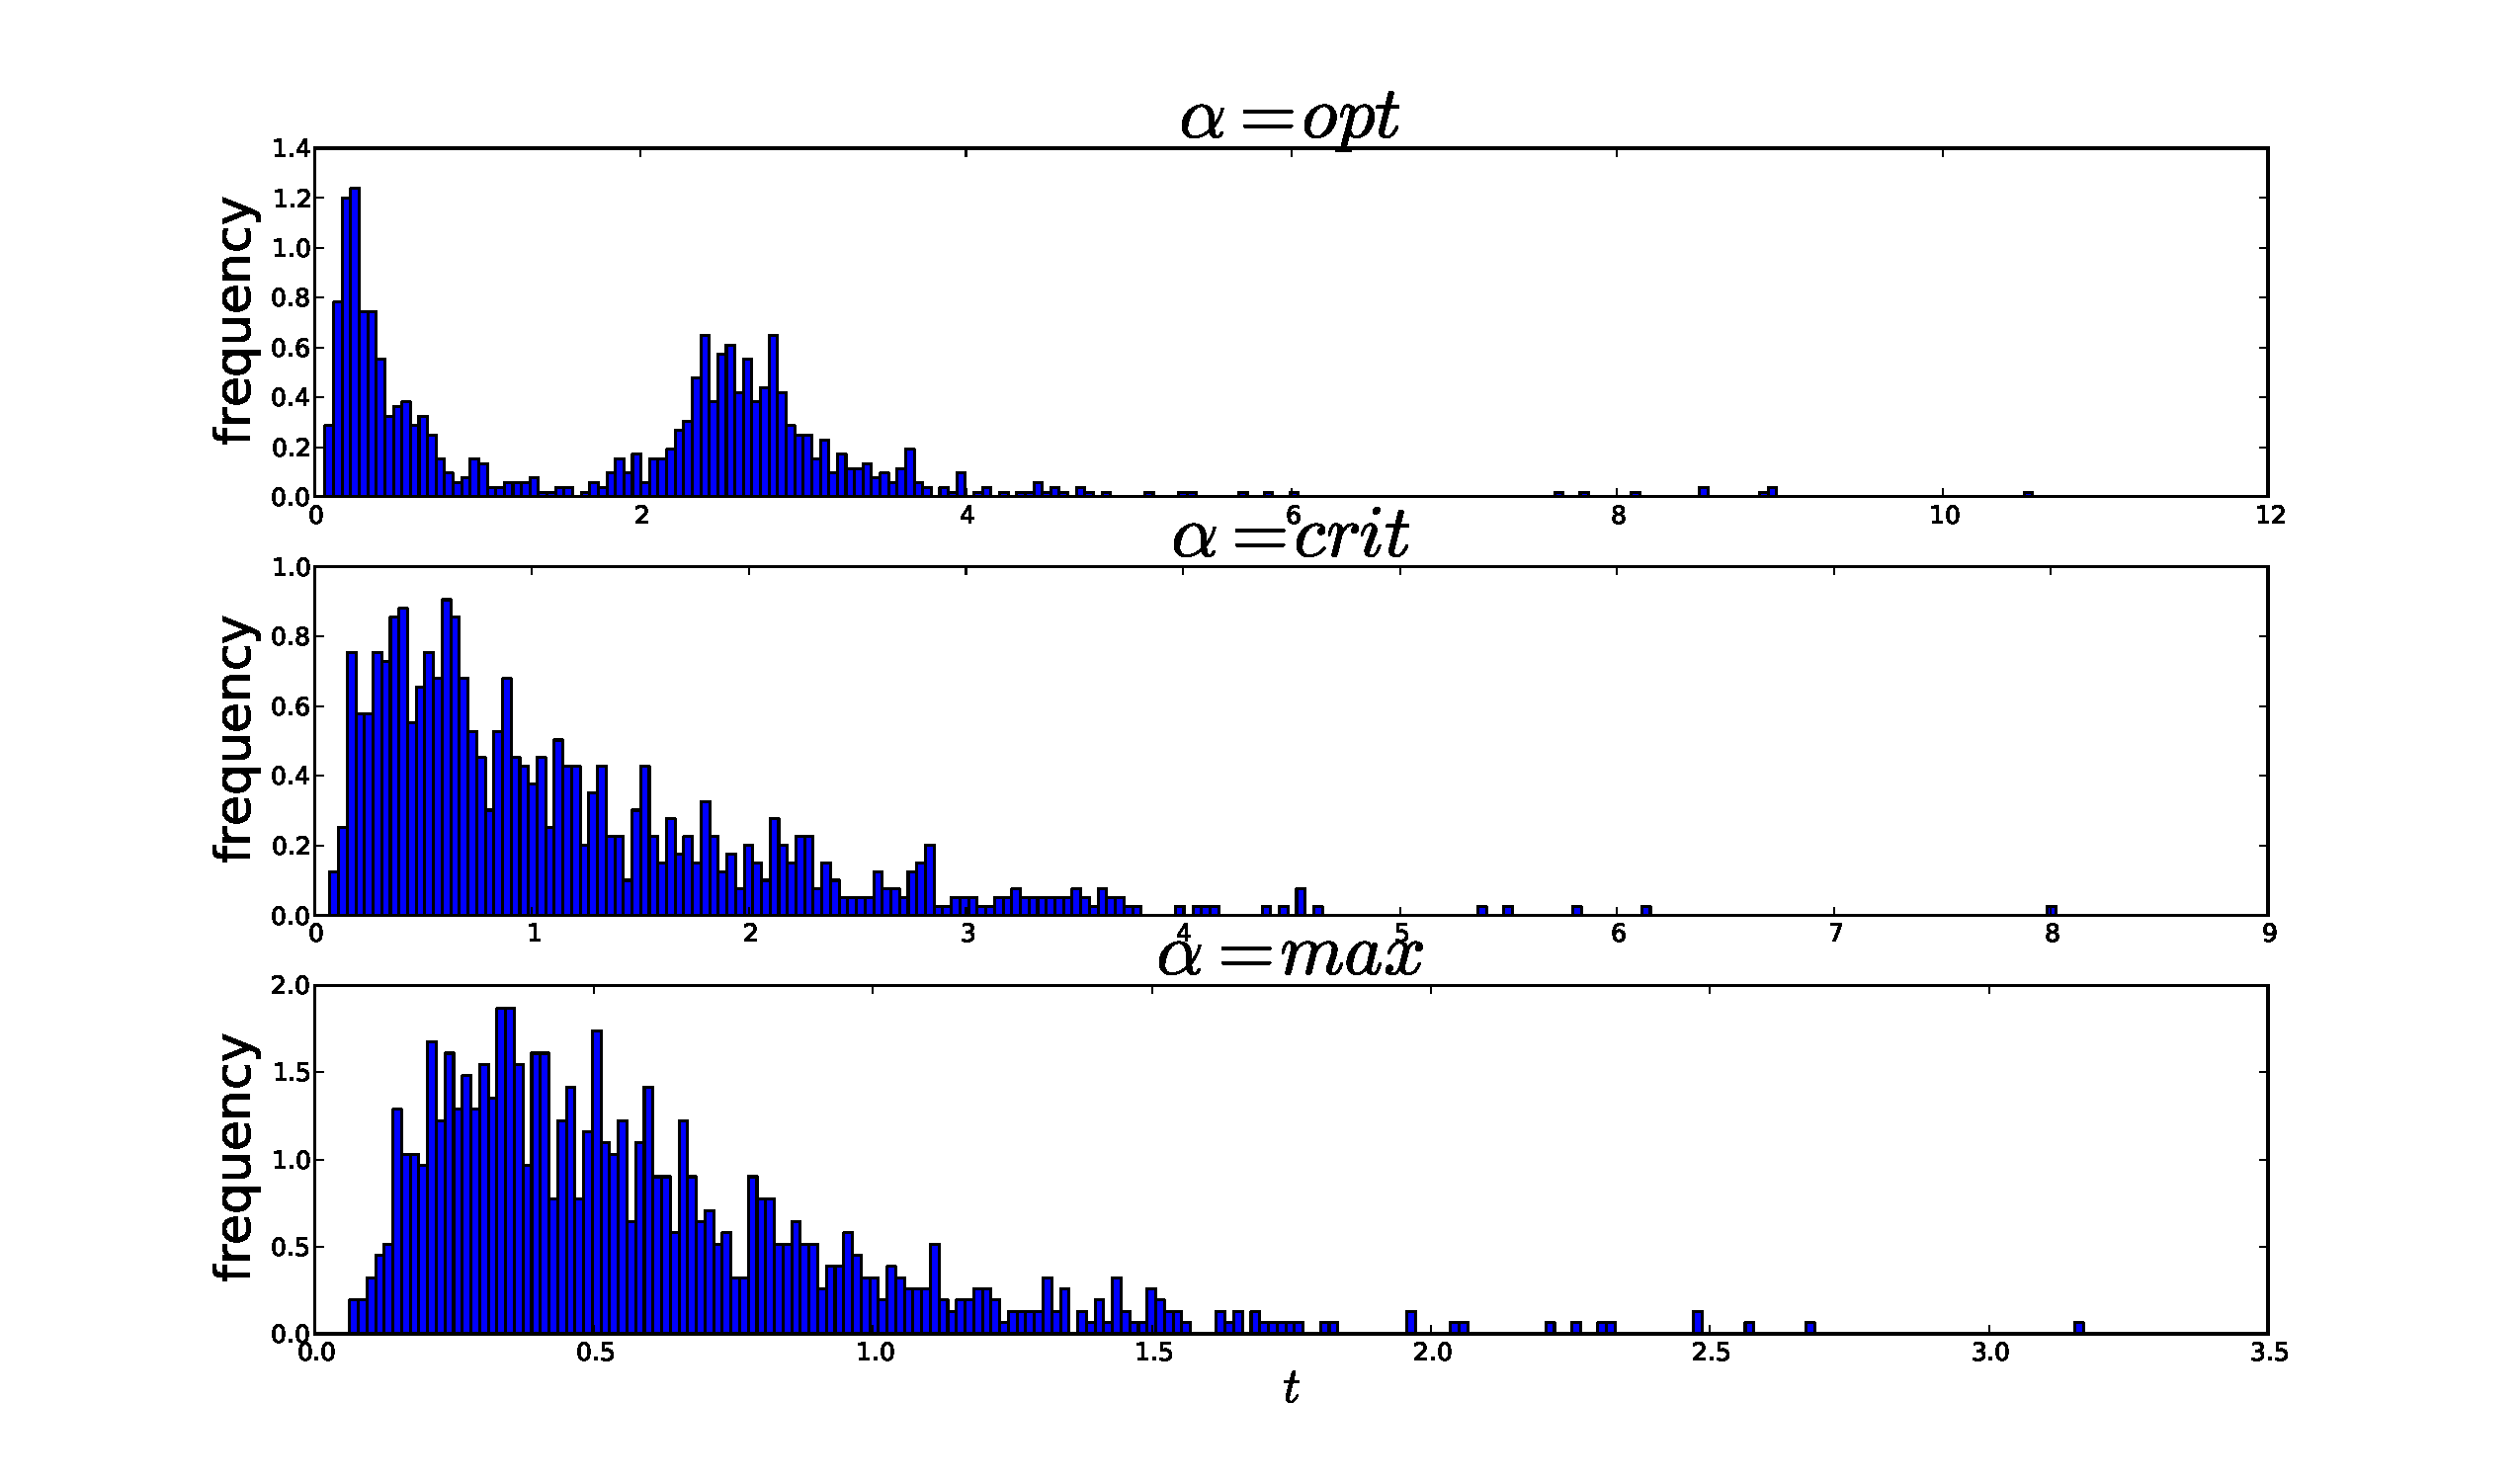
\includegraphics[width=\textwidth]{Figs/HitTime_MI_TauChar_Adjoint_Estimate/three_pt_prior_thits_distn.pdf}
%   \caption[labelInTOC]{Empirical Hitting-TIme distributions for the different
%   choices of $\a$}
%   \label{fig:empirical_hitting_times_3alphas}
% \end{center}
% \end{figure}



\begin{table}
\subfloat[$N_b=10^3, N_s = 10^2$]{
\begin{tabular}{ccc}
\input{Figs/HitTime_MI_TauChar_Adjoint_Estimate/tauchar_hit_time_100.txt}
\end{tabular}
}
\subfloat[$N_b=10^2, N_s = 10^3$]{
\begin{tabular}{ccc}
\input{Figs/HitTime_MI_TauChar_Adjoint_Estimate/tauchar_hit_time_1000.txt}
\end{tabular}
}\\
\subfloat[$N_b=10, N_s = 10^4$]{
\begin{tabular}{ccc}
\input{Figs/HitTime_MI_TauChar_Adjoint_Estimate/tauchar_hit_time_10000.txt}
\end{tabular}
} 
\subfloat[$N_b=1, N_s = 10^5$]{
\begin{tabular}{ccc}
\input{Figs/HitTime_MI_TauChar_Adjoint_Estimate/tauchar_hit_time_100000.txt}
\end{tabular}
}
\caption[Batch $\tau$ MLE estimates]{Results for the estimates arising from
simulations using various values of $\a$ (opt, crit, max). In each sub-table there are $N_b$
parameter estimates for each distinct $\a$, with $N_s$ hitting times used to
form an $\tc-$estimate.  The 'true' value of $\tc$ is $\tc=1$. Also see \cref{fig:beta_estimates_from_hitting_times_different_alphas}}
\label{tab:beta_estimates_from_hitting_times_different_alphas} 
\end{table}   

\begin{figure}[h]
\begin{center}
\subfloat[$N_b=10^3, N_s = 10^2$]
{
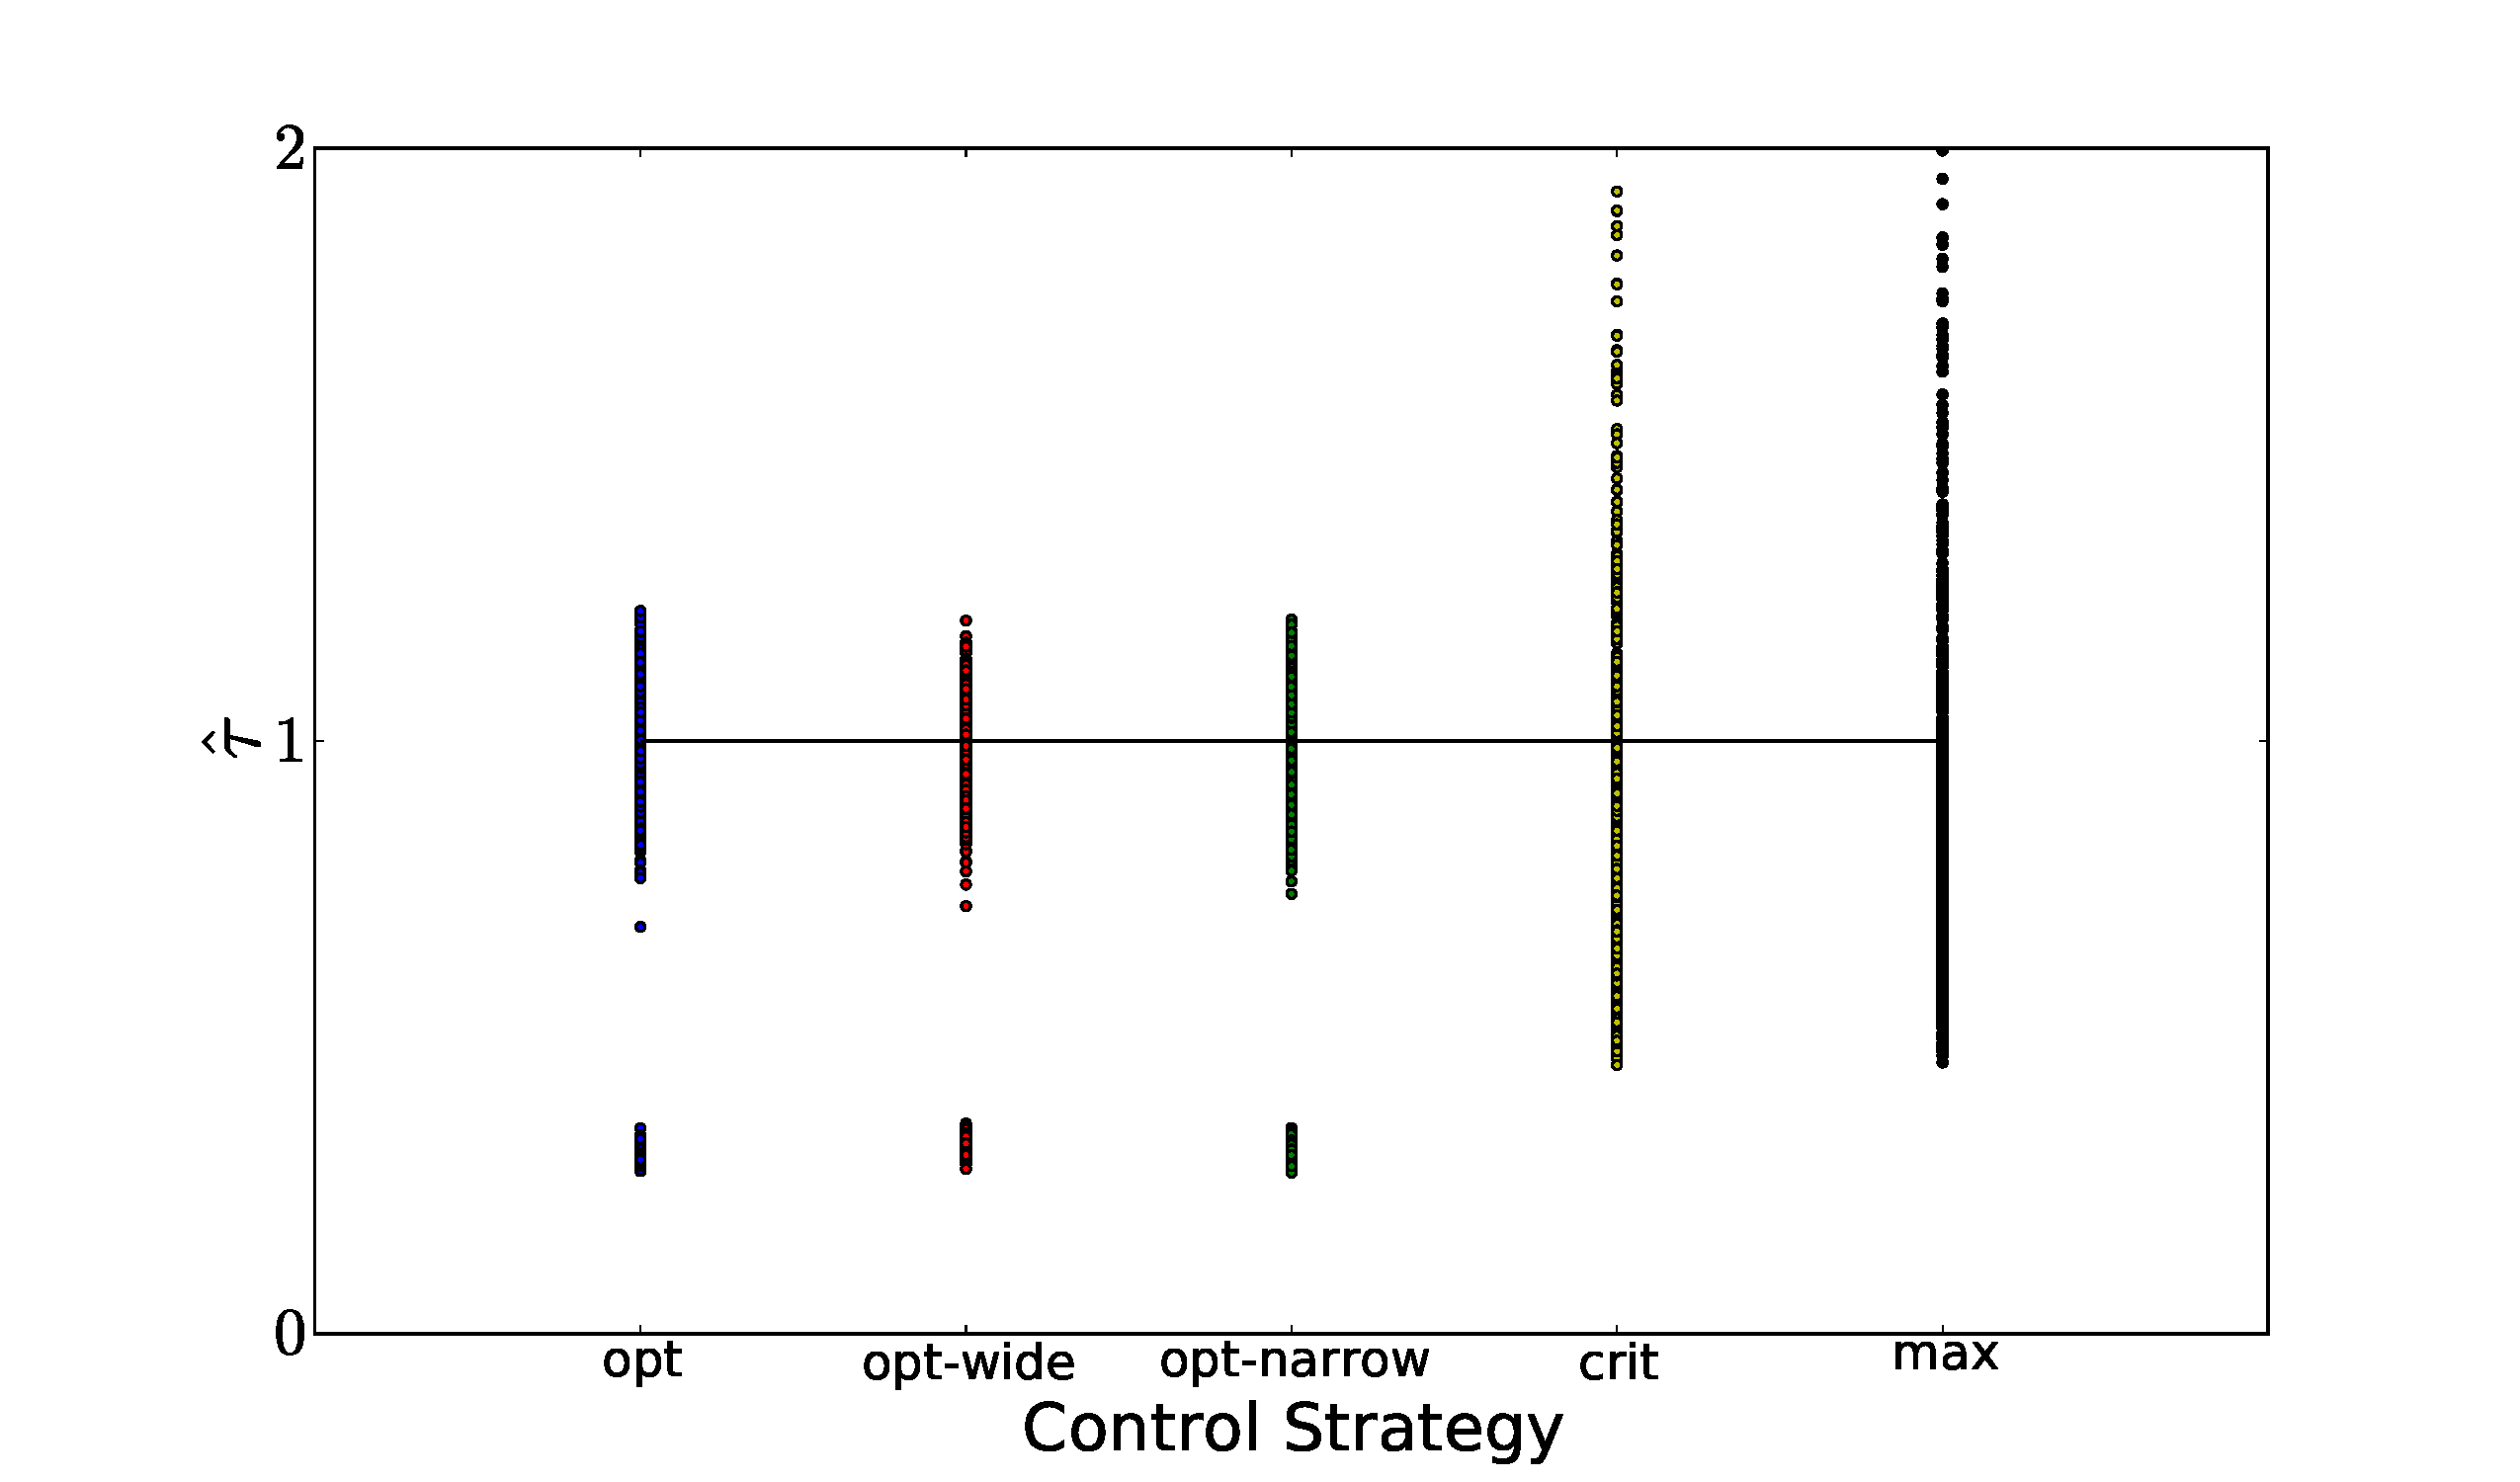
\includegraphics[width=0.48\textwidth]
{Figs/HitTime_MI_TauChar_Adjoint_Estimate/miestimates_scatterplot_Nb1000_Ns100.pdf}
}
\subfloat[$N_b=10^2, N_s = 10^3$]
{
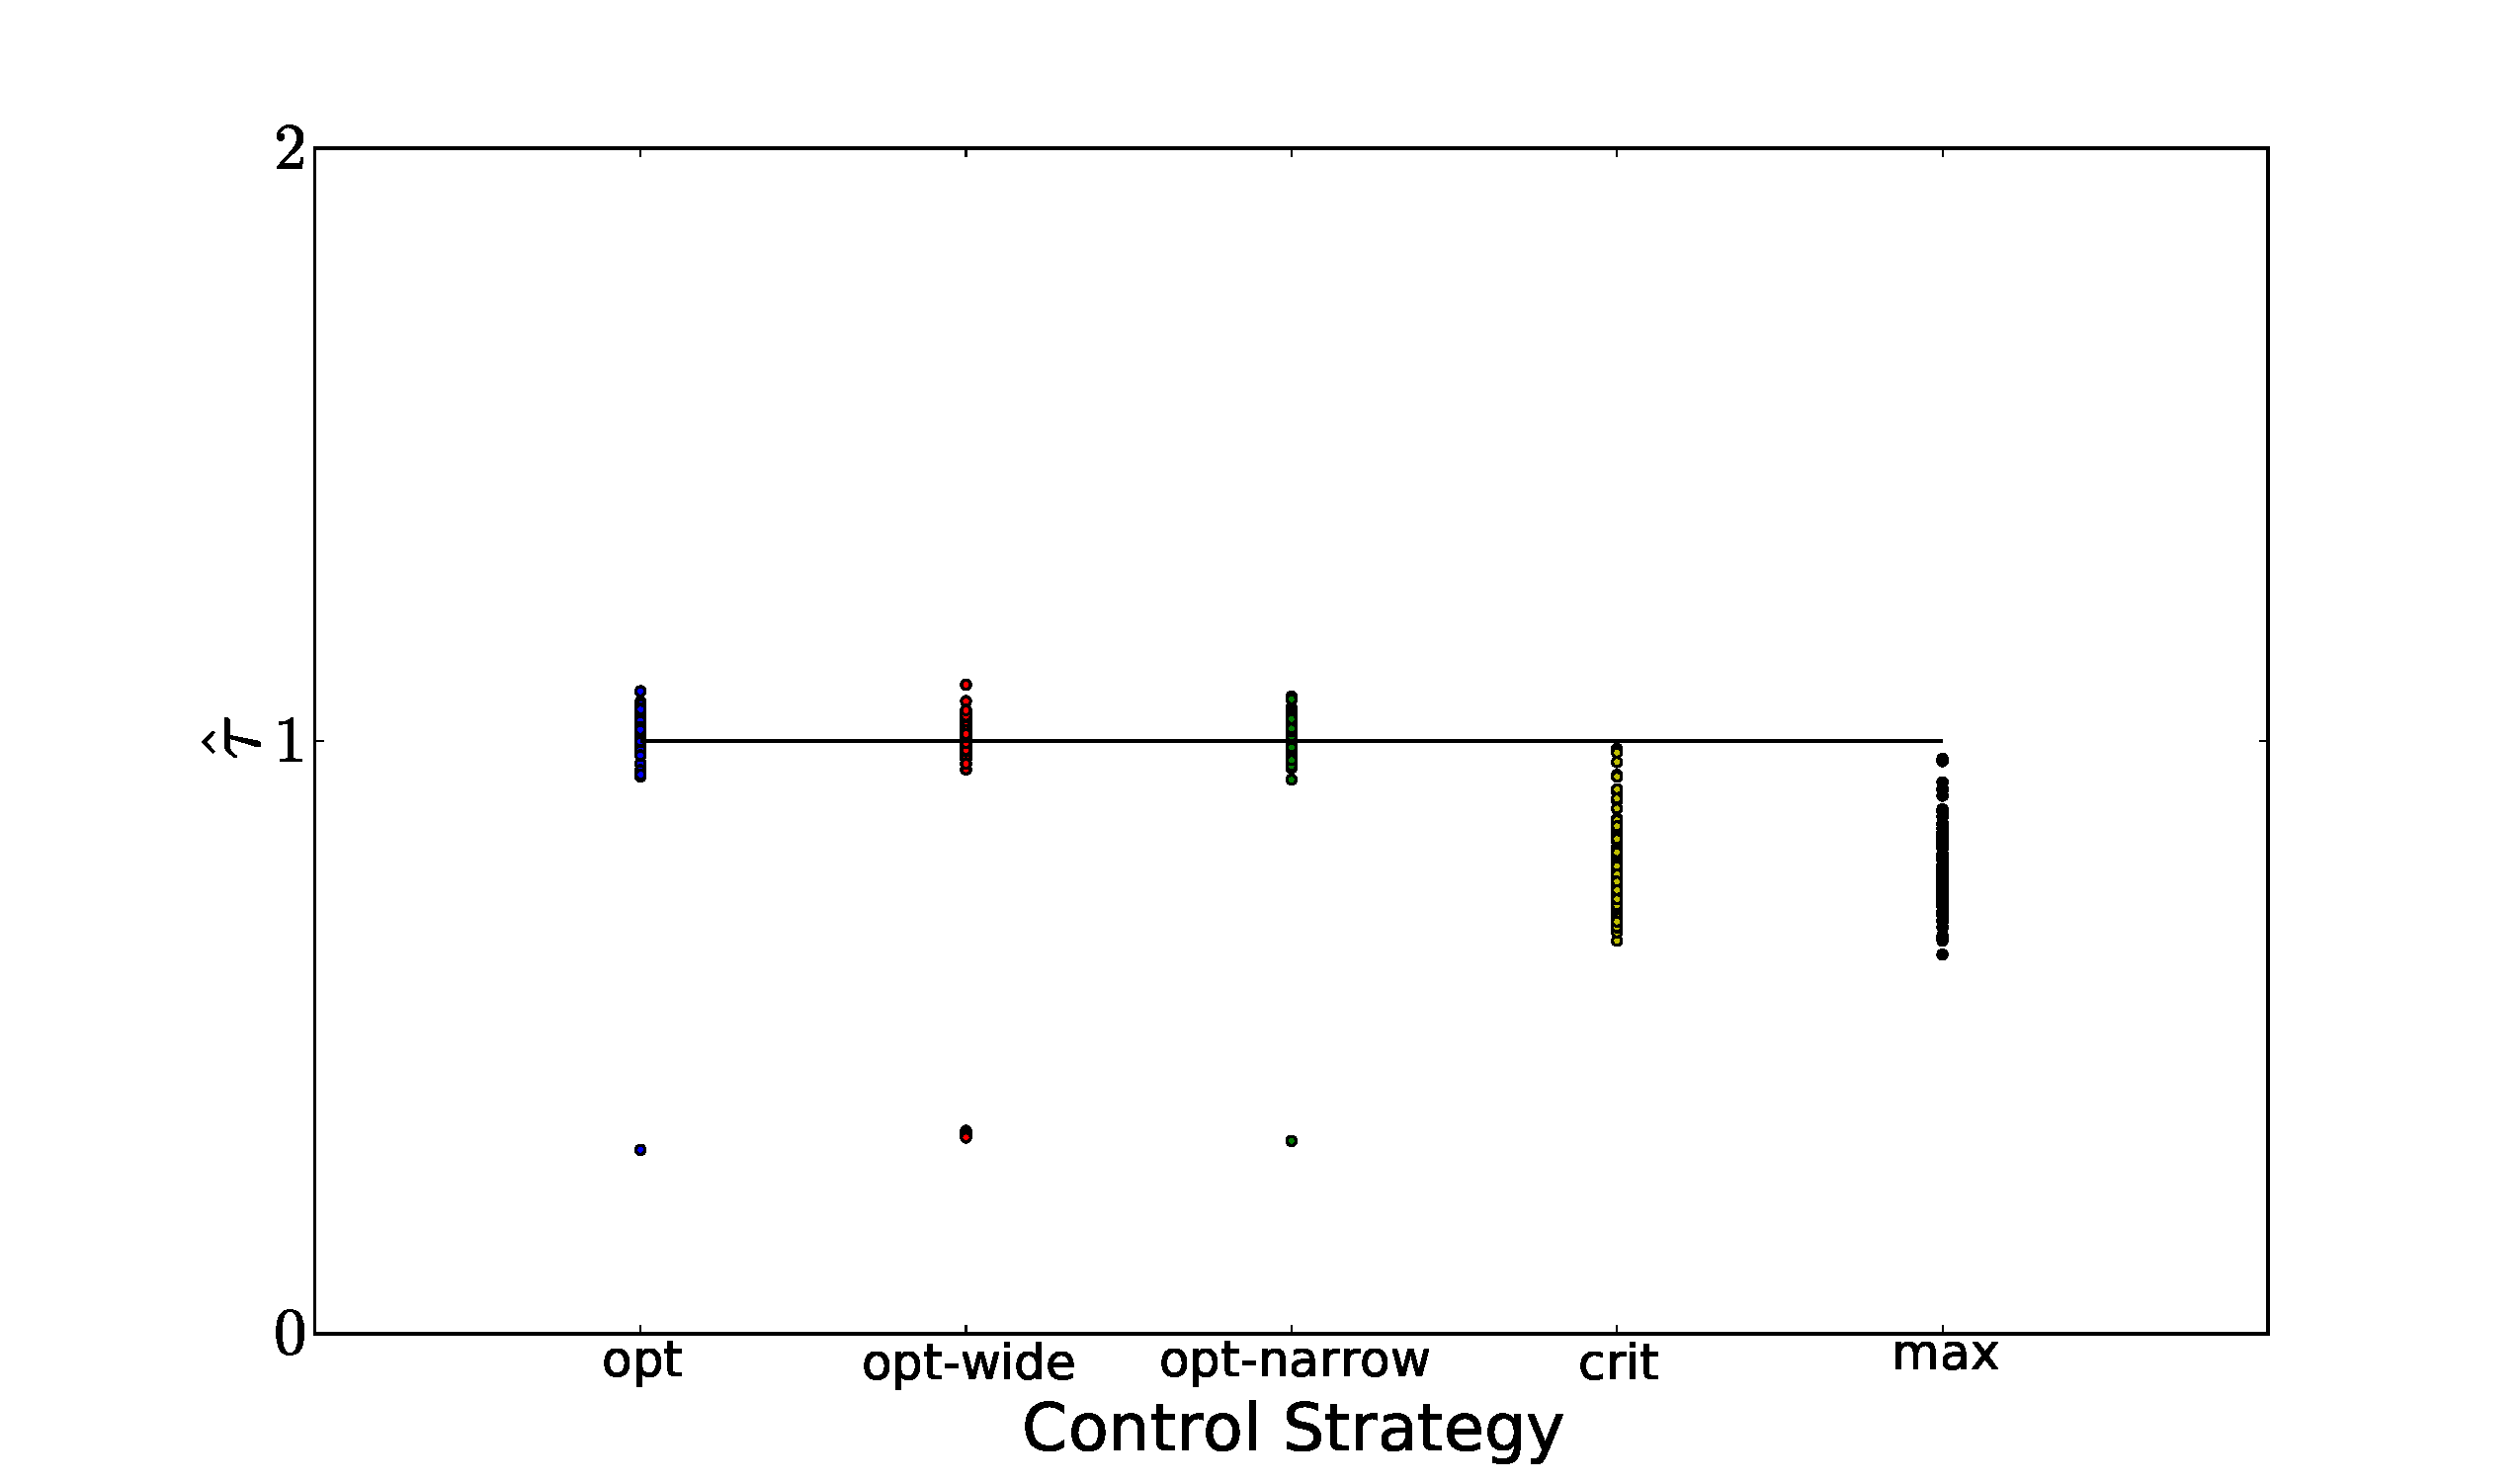
\includegraphics[width=0.48\textwidth]
{Figs/HitTime_MI_TauChar_Adjoint_Estimate/miestimates_scatterplot_Nb100_Ns1000.pdf}
}
\\
\subfloat[$N_b=10^2, N_s = 10^4$]  
{
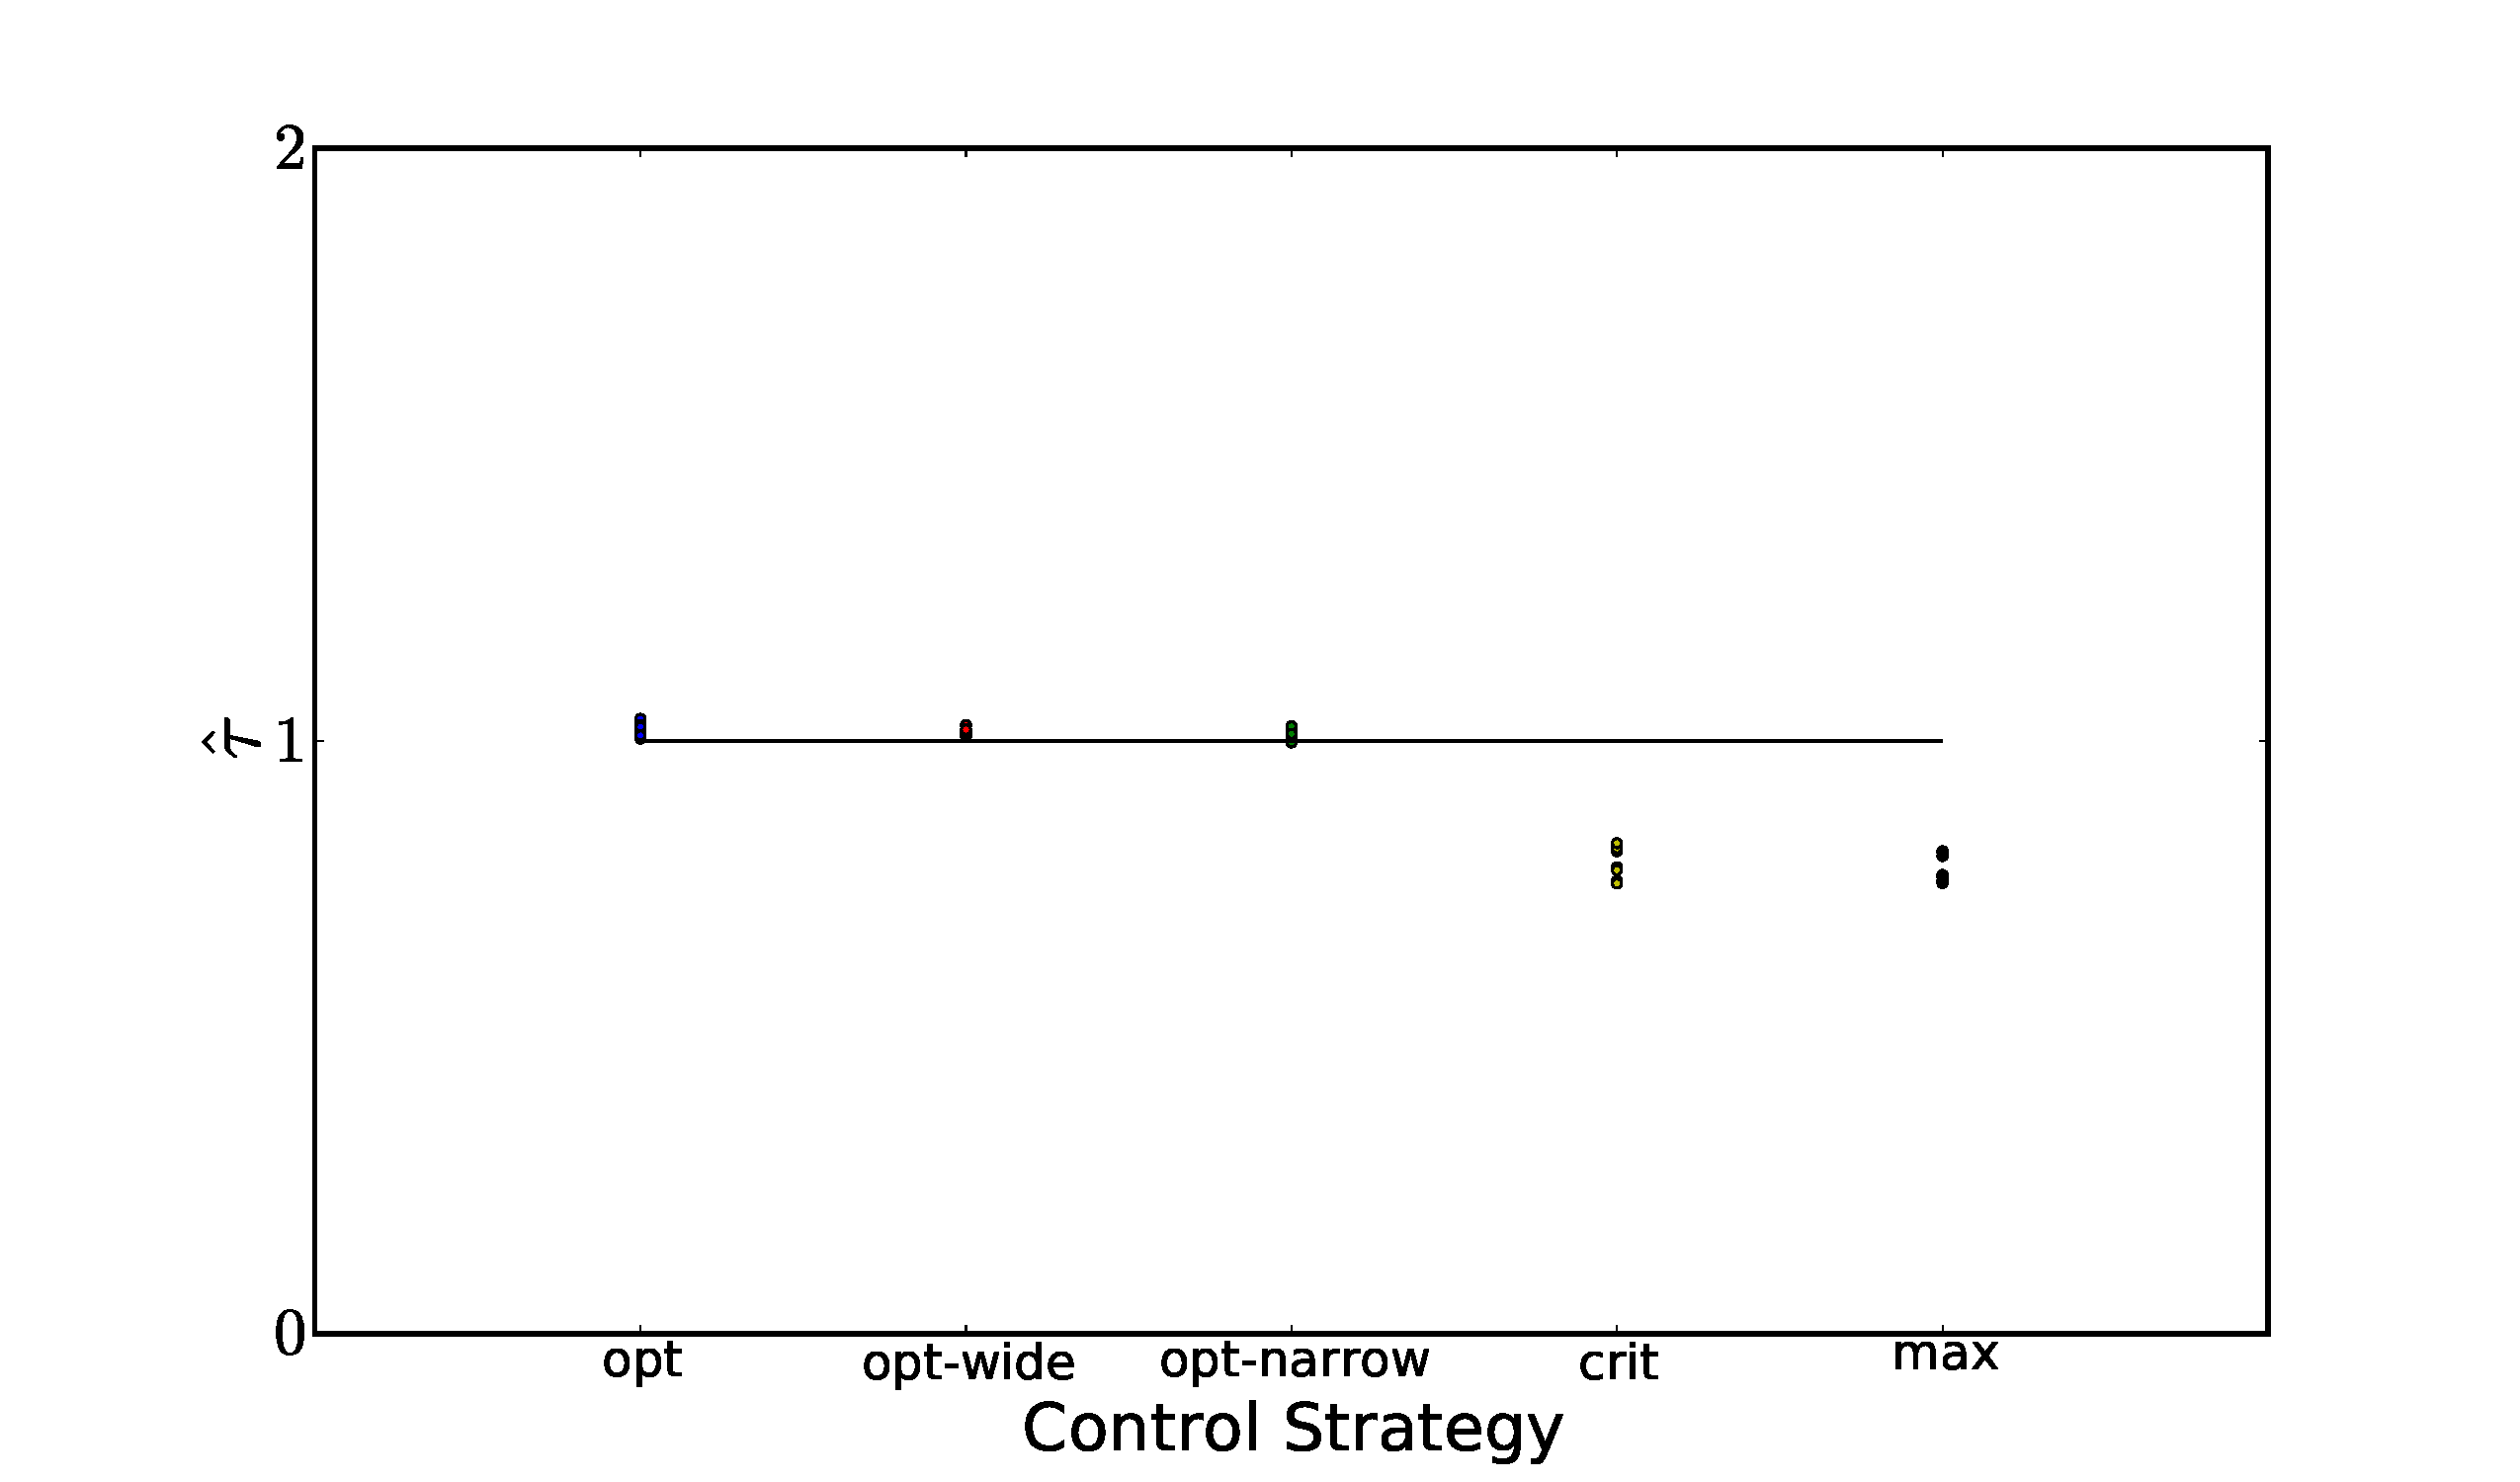
\includegraphics[width=0.48\textwidth]
{Figs/HitTime_MI_TauChar_Adjoint_Estimate/miestimates_scatterplot_Nb10_Ns10000.pdf}
}  
\subfloat[$N_b=1e1, N_s = 10^5$]
{ 
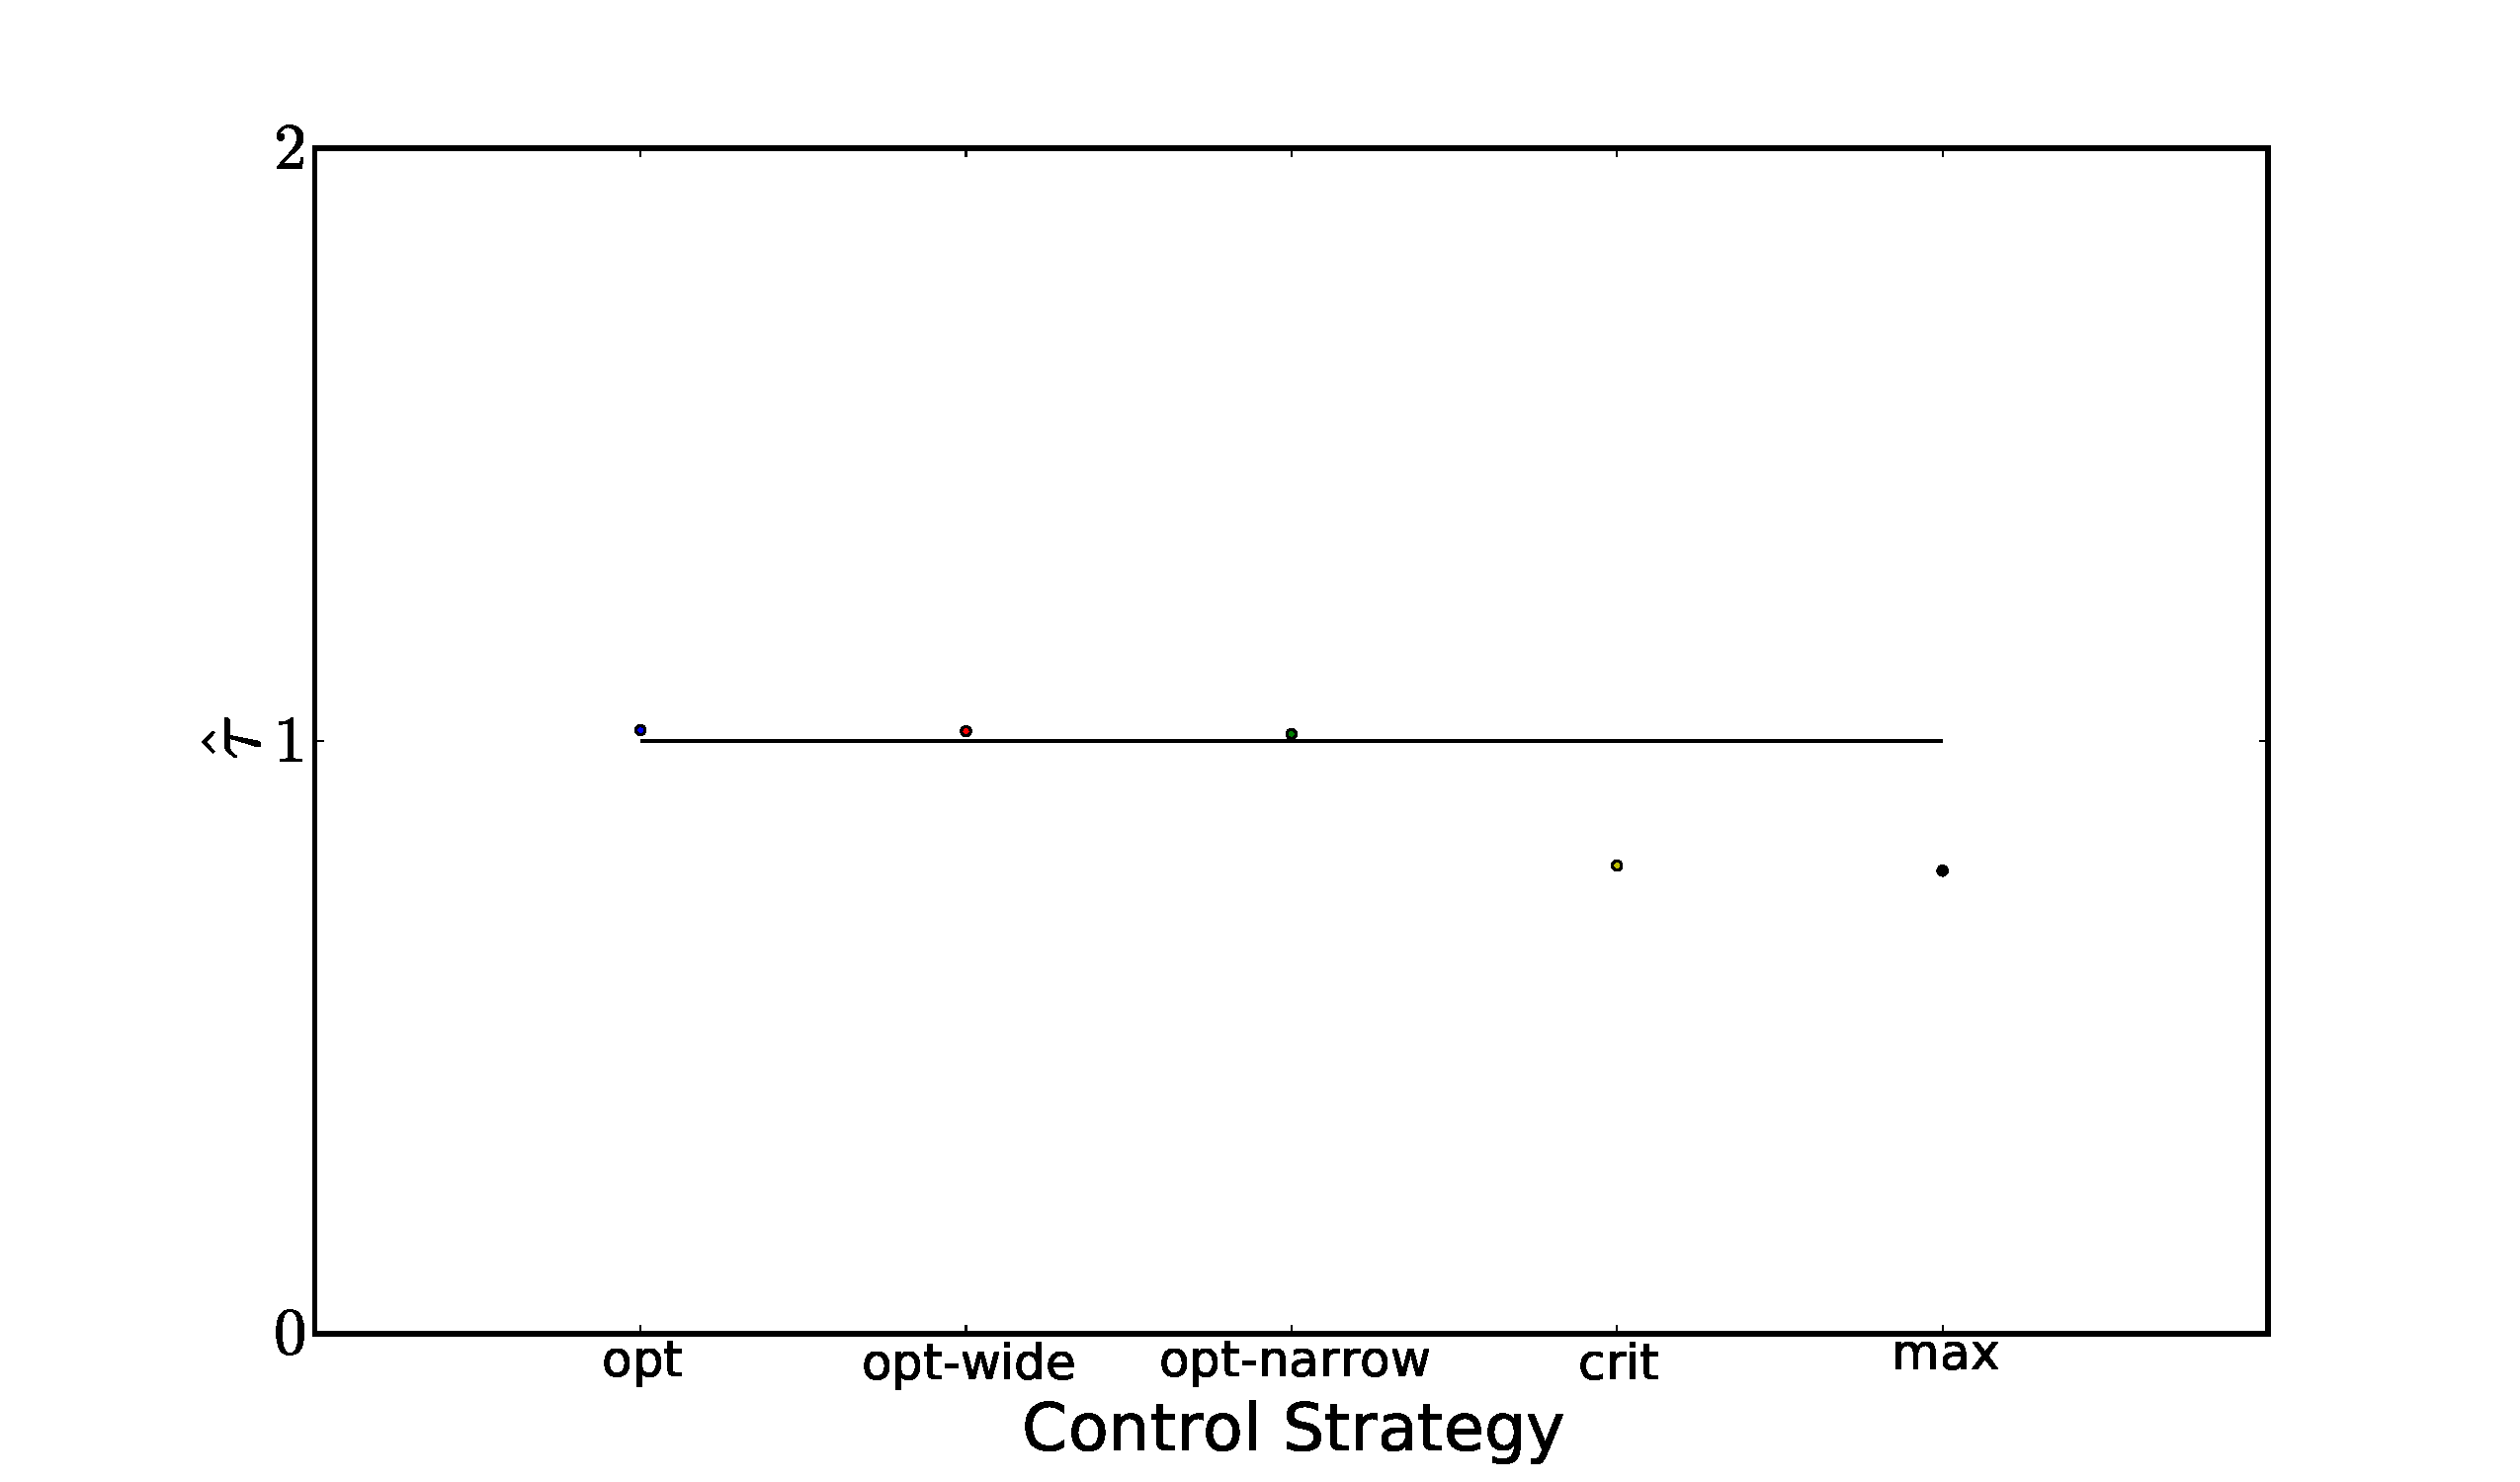
\includegraphics[width=0.48\textwidth]
{Figs/HitTime_MI_TauChar_Adjoint_Estimate/miestimates_scatterplot_Nb1_Ns100000.pdf}
}
\caption[Illustration of the individual MLE Estimates]{Fine Visualization of the
MLE estimates for the different controls, also see
\cref{tab:beta_estimates_from_hitting_times_different_alphas}}
\label{fig:beta_estimates_from_hitting_times_different_alphas}
\end{center}
\end{figure} 
 
Together
\cref{tab:beta_estimates_from_hitting_times_different_alphas,fig:beta_estimates_from_hitting_times_different_alphas}
confirm a clear advantage to using the Optimal Control, $\a_{opt}$ over the
simpler, constant controls. In particular, the bias of the estimates is
significantly reduced. 
% (ALEX: greater than what? and I see the variance being smaller for opt cases) 
In fact the statistics in
\cref{tab:beta_estimates_from_hitting_times_different_alphas}, especially in
panel a) tend to be skewed due to the presence of a few outlier estimates for
the optimal control. This can be seen in the detailed distribution of estimates,
shown in the top panels in
\cref{fig:beta_estimates_from_hitting_times_different_alphas}.
Meanwhile, if we consider the various optimal
controls, 'opt' vs. 'opt-wide' or 'opt-narrow', we see that there is no big
difference in the estimator quality of each - they all perform approximately
equivalently.

\begin{figure}[h]
\begin{center} 
\subfloat[10^3 Hits]   
{ 
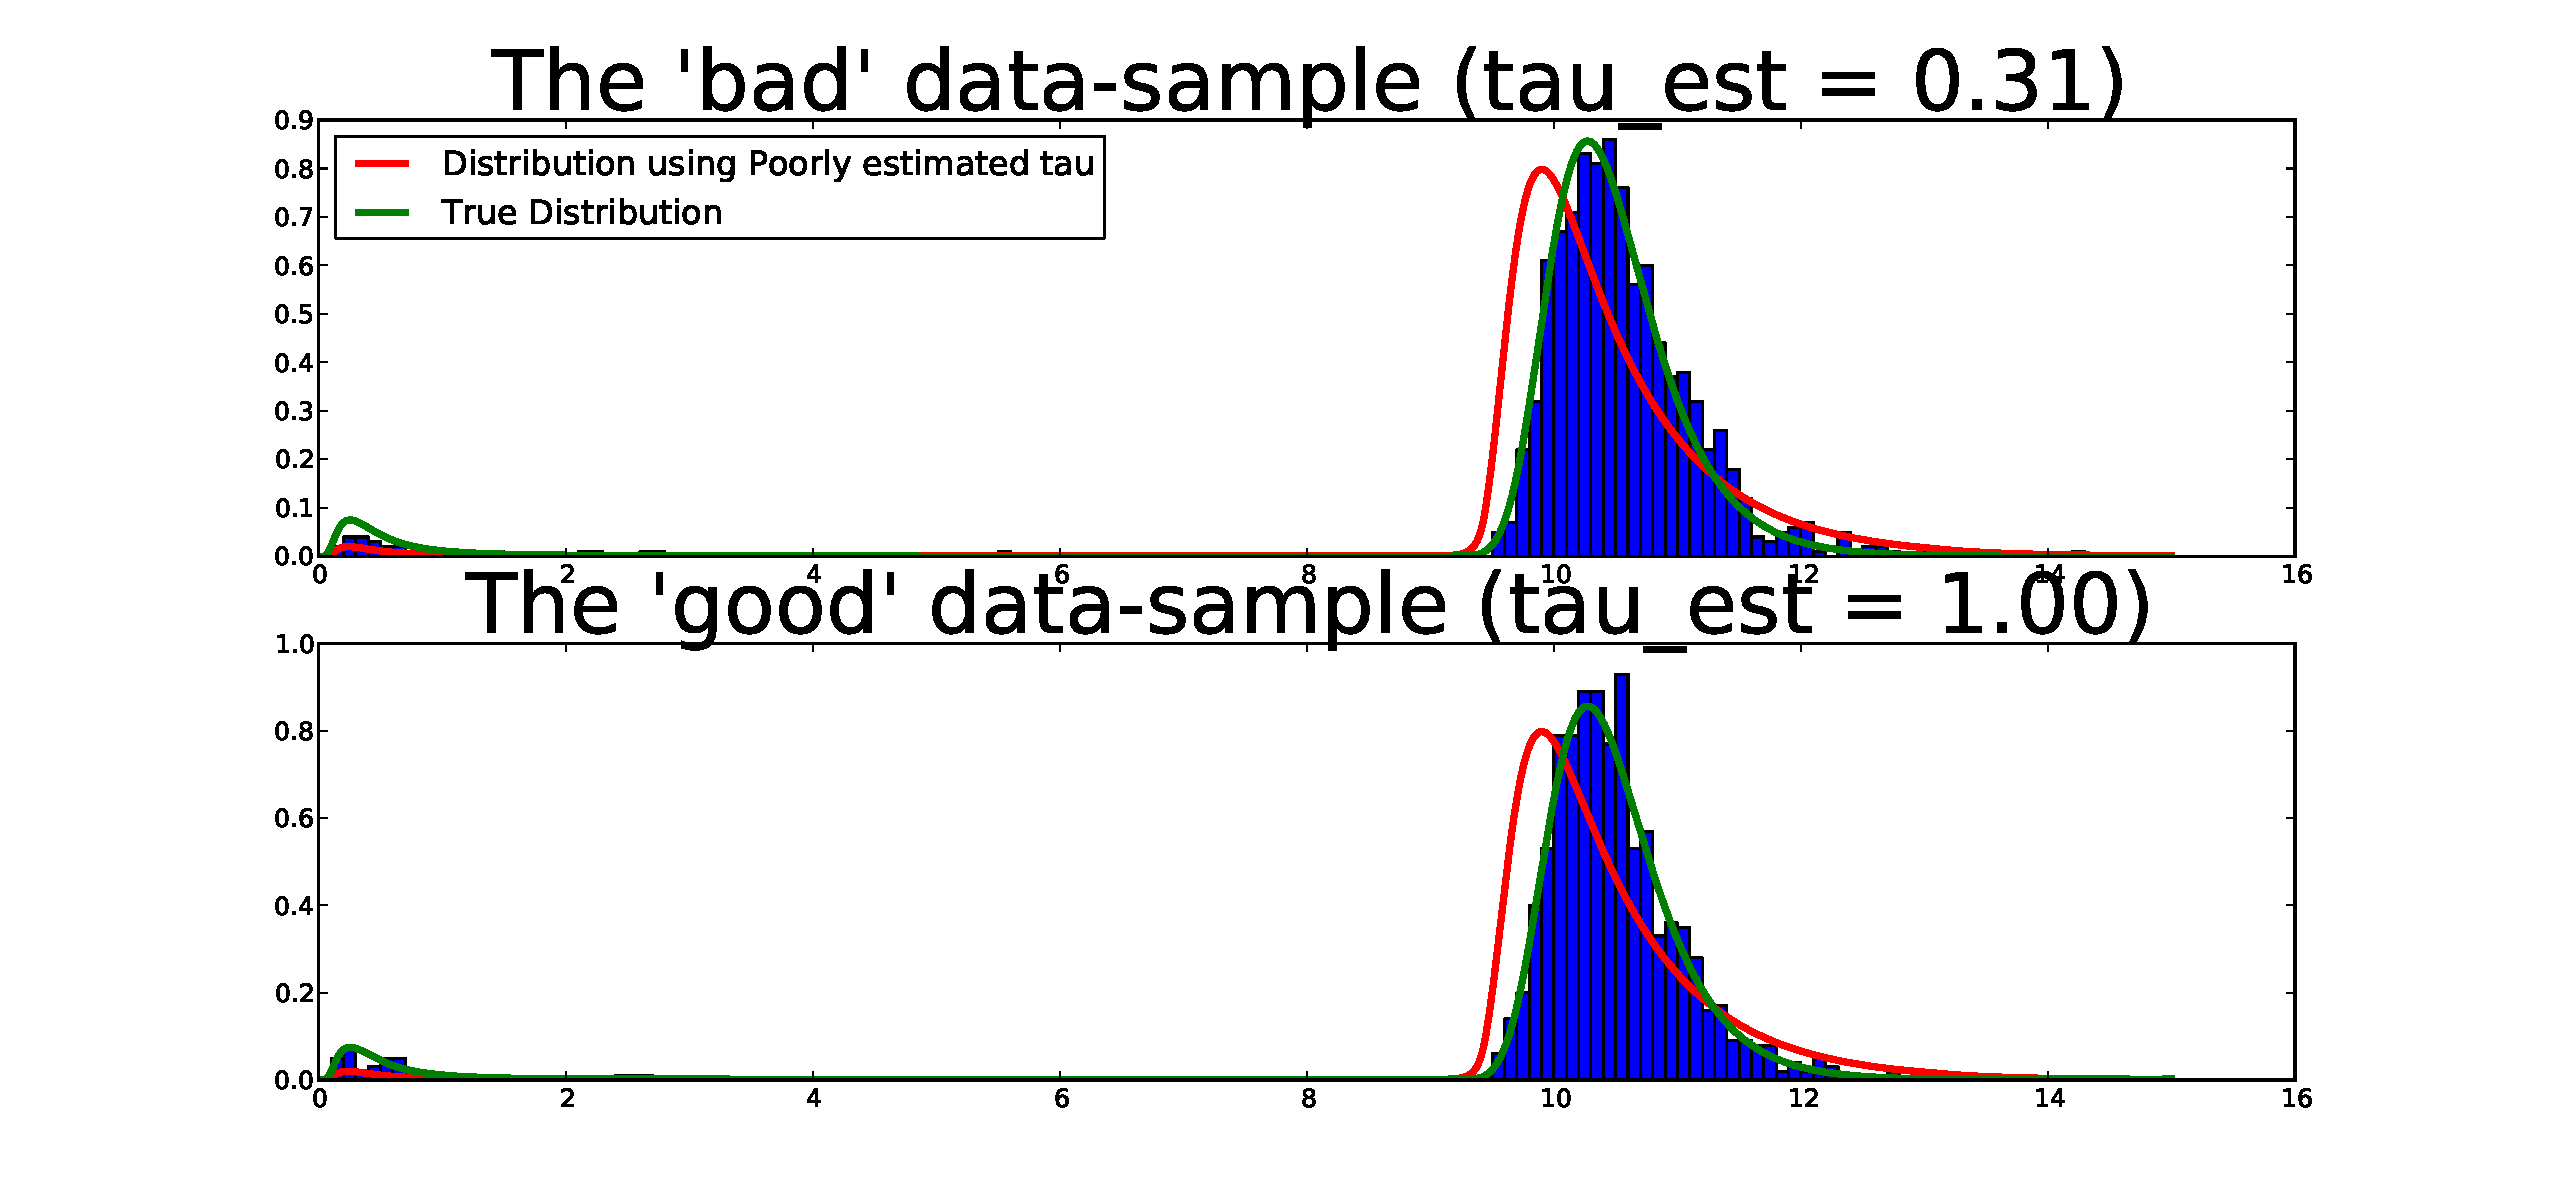
\includegraphics[width=0.98\textwidth]
{Figs/HitTime_MI_TauChar_Adjoint_Estimate/Adjoint_TauChar_Estimator_good_vs_bad_estimates_Nh1000.pdf}
}\\
\subfloat[10^4 Hits]
{
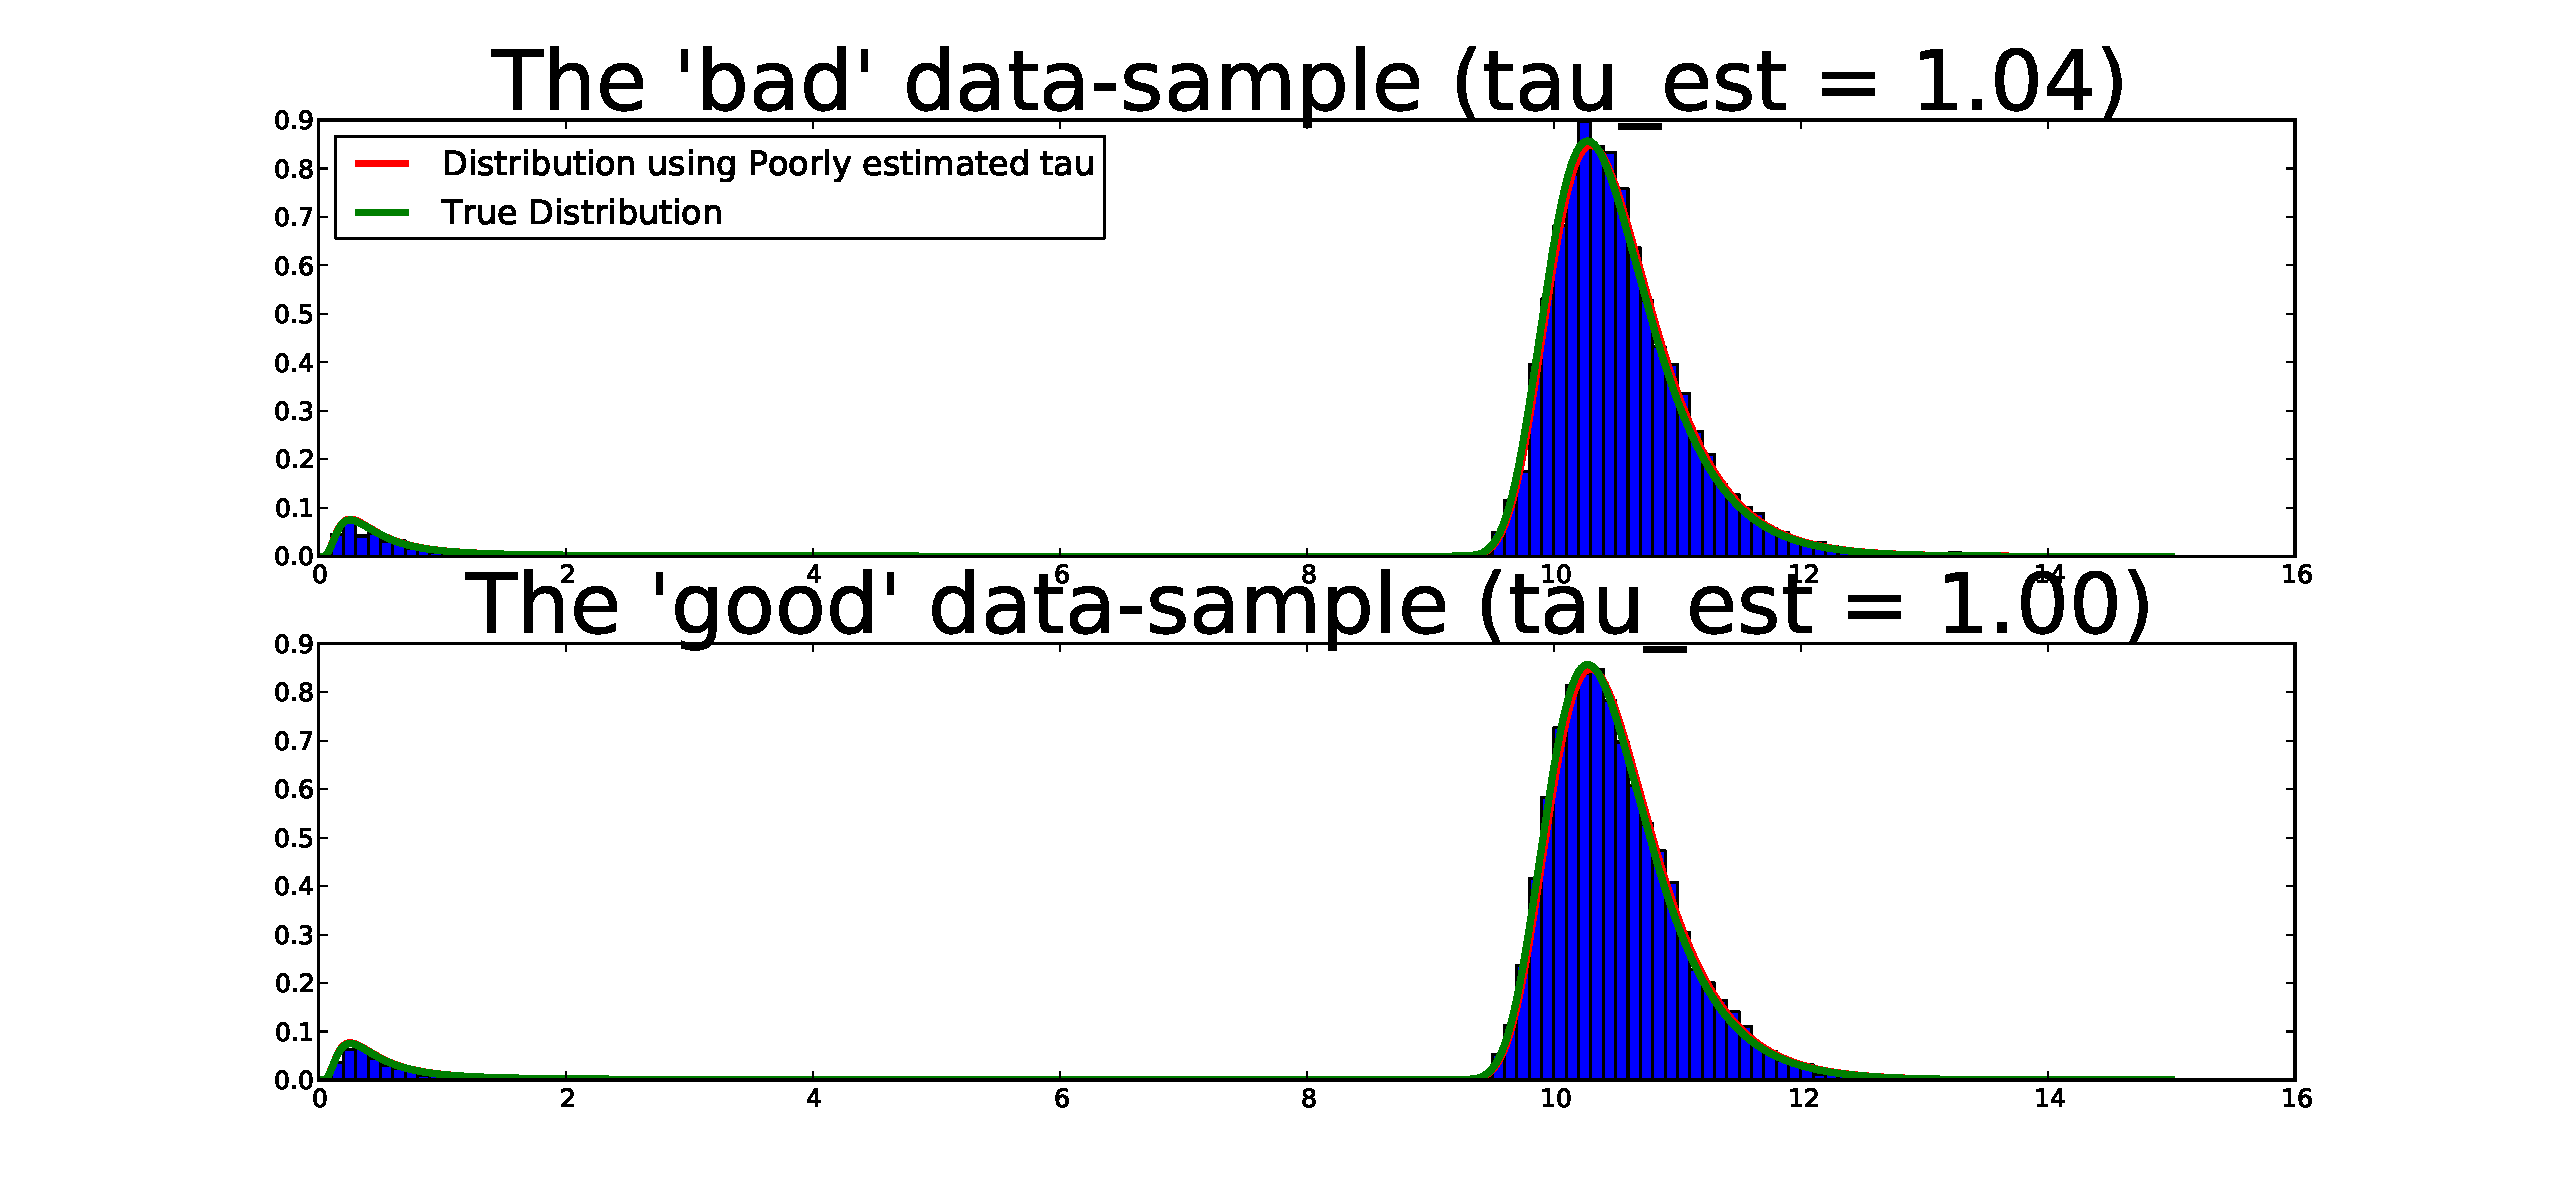
\includegraphics[width=0.98\textwidth]
{Figs/HitTime_MI_TauChar_Adjoint_Estimate/Adjoint_TauChar_Estimator_good_vs_bad_estimates_Nh10000.pdf}
}
\caption[Estimation Detail View for the Optimally-Stimulated
Experiment]{Comparing the case when the estimation does best vs. when it does
worst for the optimally-stimulated experiment. In the case with less samples, a
few extreme observations can skew the estimate, however with more data points,
those are seen to be rare cases and a more accurate estimate is found.}
\label{fig:batch_estimtion_in_detail}
\end{center}
\end{figure}


\subsection{Proof of concept for estimating the entire parameter set}
% (ALEX: Proof of concept section which goes here reads well.
%  I would change the title to "Proof of concept for estimating the entire
%  parameter set".
% I would replace "essentially irrelevant" to "largely insensitive " 
% Replace "introduction" by "Introduction". 
% replace "removing variation from one parameter...variation" to 
% "reducing fluctuations in one parameter...fluctuations...". 
% And replace "necessarily removes" by "is
%  expected to remove". Also, no paragraph here: "...we make 10 estimates. The
%  results in fig.9 make it clear that the 'optimally' stimulated samples yield
%  much more accurate.."
% Also remove the second "in particular" and start that sentence with "The naive
% stimulation..." "while the dynamic, bang-bang situation": while the dynamic
% situation that results in a bang-bang-like optimal control... caption fig.9:
% per-estimate : remove hyphen

So far we have assumed that $\mu, \s \in \th$ are known. We now relax that
assumption and attempt to estimate those two parameters in addition to
characteristic time $\tc$. We still use the optimal control obtained assuming
$\m,\s$ known. Why is this expected to work? First of all we found that the
optimal control seems largely insensitive to the exact values of $\m,\s$ as long
as they are not 'too far' from the nominal values ($\m=0, \s=1$.). Moreover as
discussed in the Introduction, the $\tc$ parameter is well-known to be the
hardest to estimate. Thus a scheme designed to estimate it well is conjectured
to help with estimation of the entire parameter set, since reducing fluctuations
from one parameter estimate is expected to reduce fluctuations from the others.
We use the same simulated hitting-time data-set as in
\cref{tab:beta_estimates_from_hitting_times_different_alphas,fig:beta_estimates_from_hitting_times_different_alphas},
using $N_s=10^4$ hits and $N_b=10$ separate sample-sets, i.e.\ we make 10
estimates. The results in \cref{fig:all_theta_estimates_batch} make it clear
that the 'optimally' stimulated samples yield much more accurate and precise
estimates. In particular all stimulation schemes come-up with high-fidelity
estimates for $\s$; it is in resolving the interplay between $\m,\tc$ that the
'optimal' stimulation excels. The 'naive' stimulations do not
allow to distinguish a high $\m$ and a small $\tc$ from a low $\m$ and a high
$\tc$, while the dynamic stimulation that results in a bang-bang-like optimal
control makes it possible. \begin{figure}[htp]
\begin{center}
  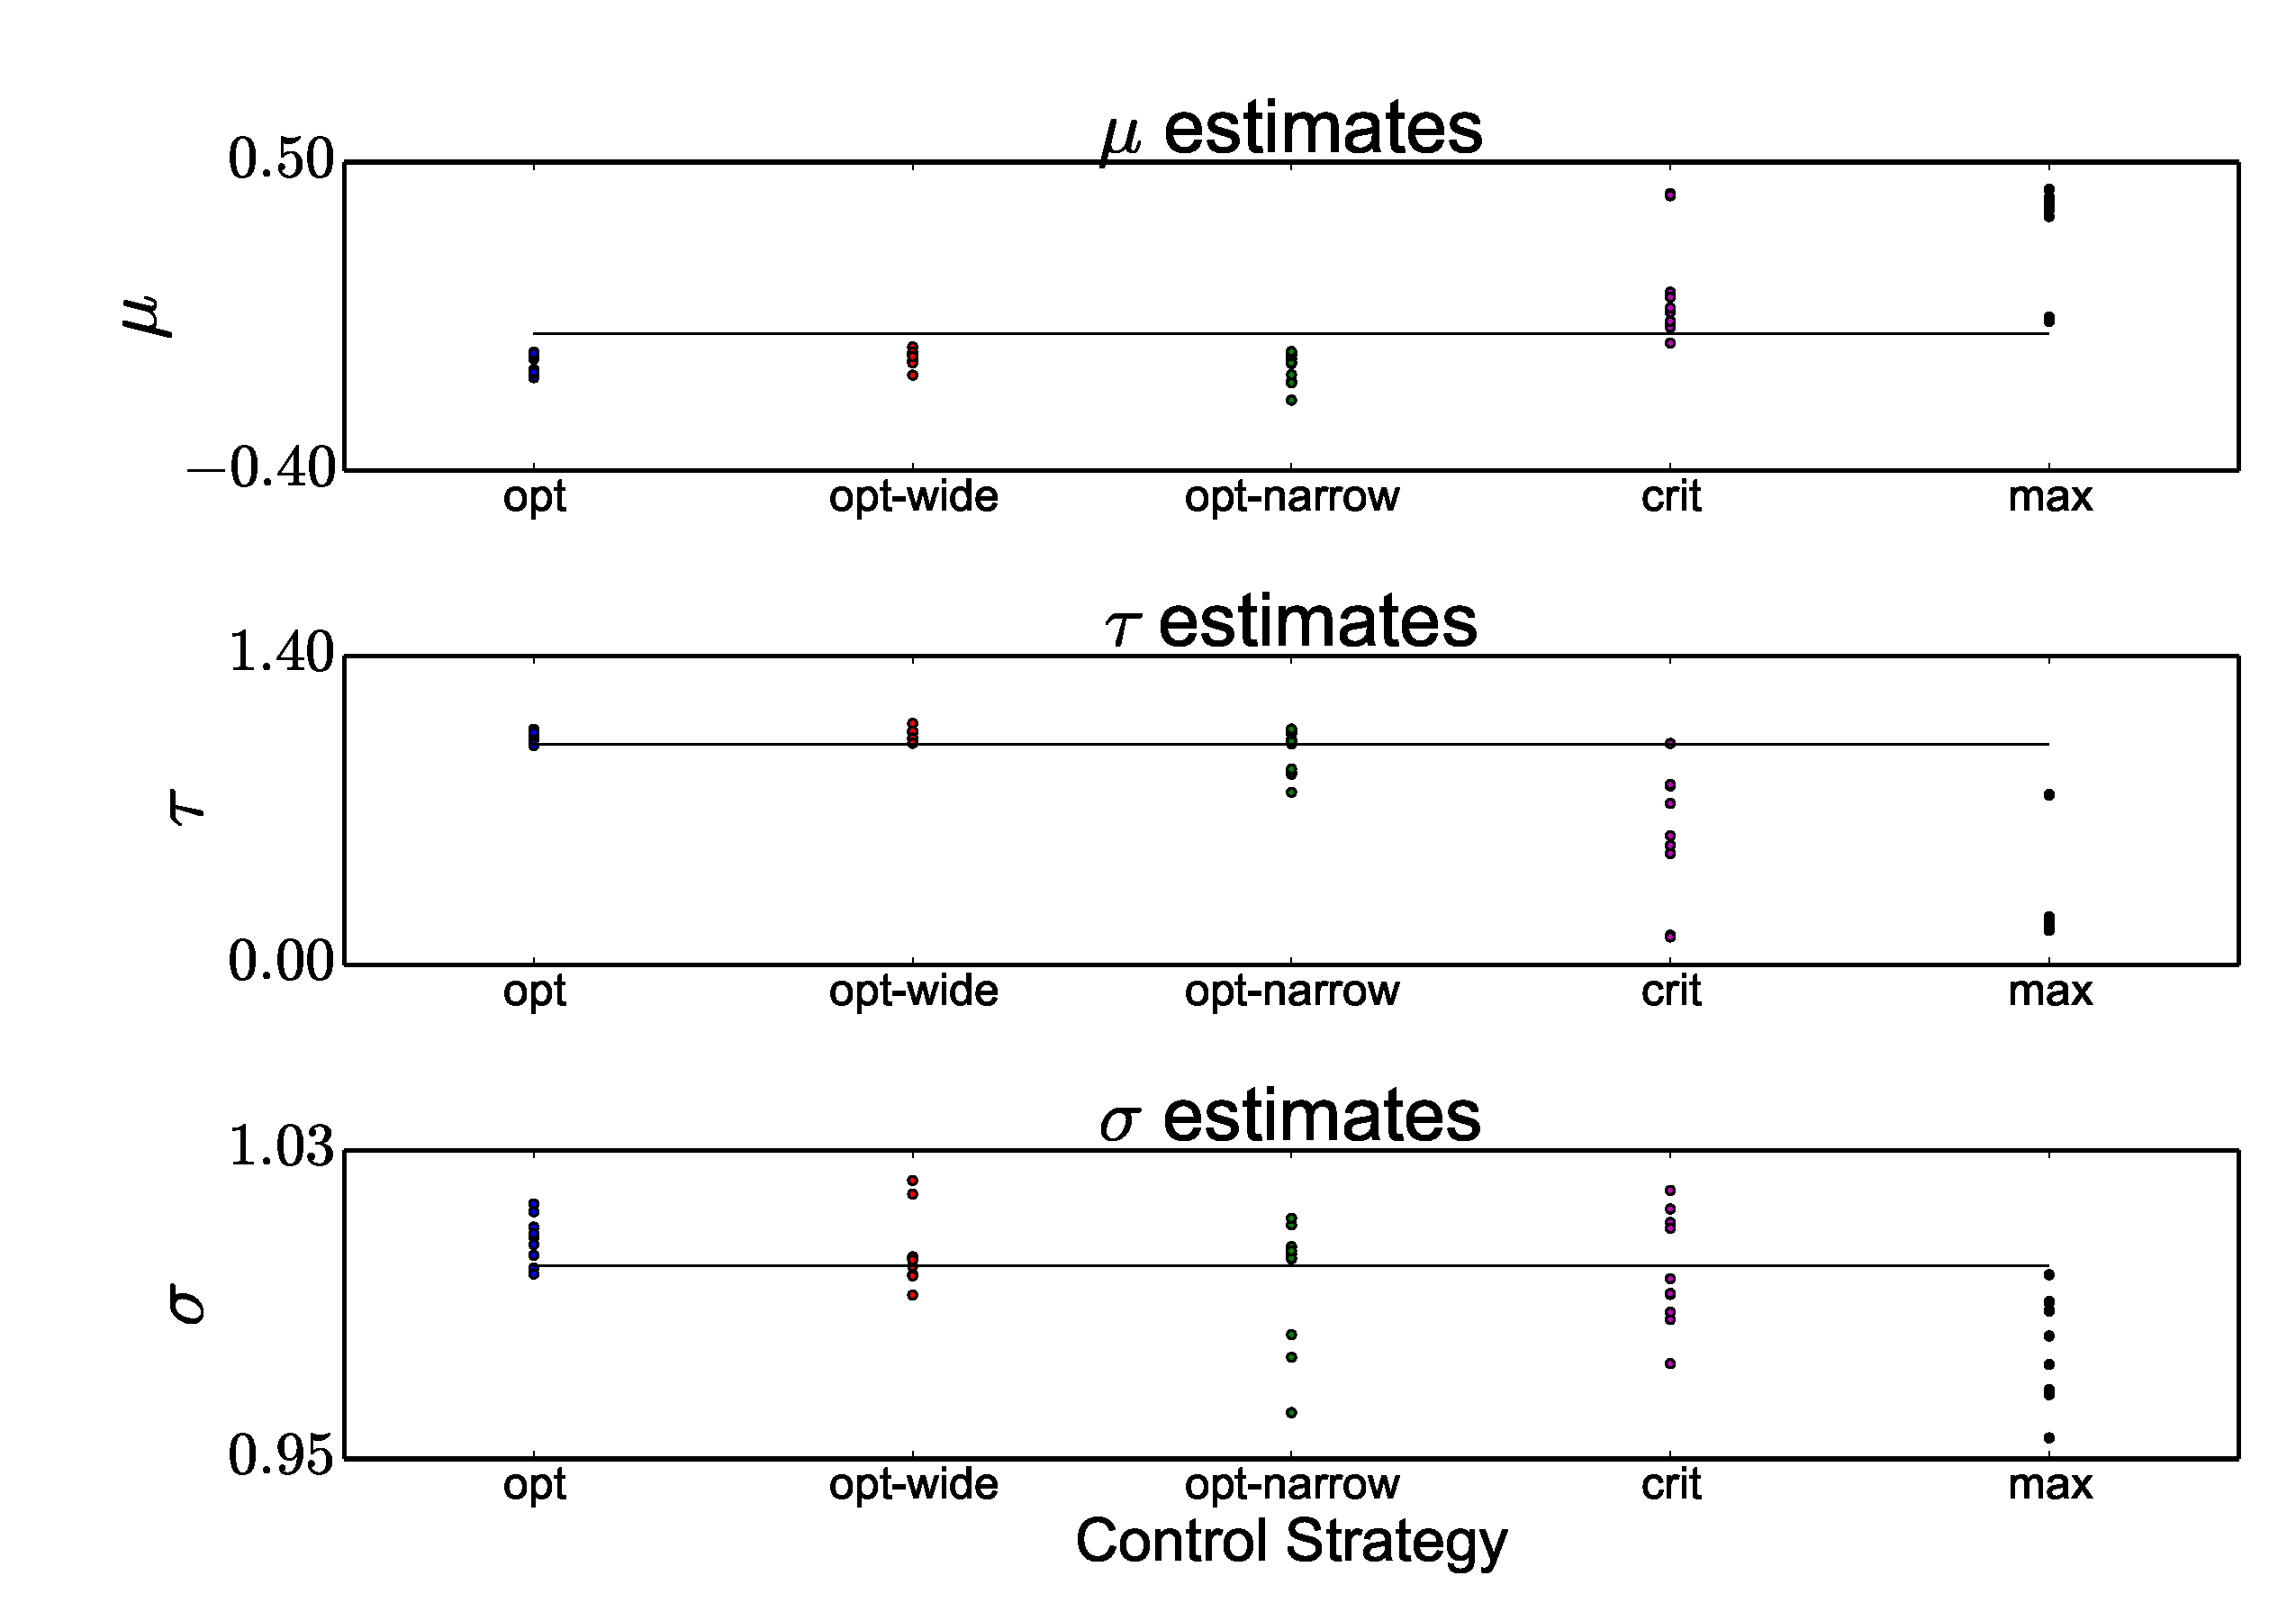
\includegraphics[width=\textwidth]{/home/alex/Workspaces/Latex/OptEstimate/Figs/MuTauSigma_Batch_estimates/all_theta_estimates_scatterplot_Nb10_Ns10000.pdf}
  \caption[Batch estimates for all 3 parameters]{Optimal Stimulation greatly
  improves estimates when all parameters are being estimated. 
  From the top to bottom, we show $N_b=10$ estimates for $\m,\tc,\s$,
  formed after observing $N_s=10^4$ hits per estimate. There are three 'optimal'
  stimulations as discussed in the text, shown to the left and two naive ones,
  shown to the right. The scatter dots are the individual estimates per
  stimulation-parameter pair. The horizontal line indicates the true value of
  the parameters, i.e.\ the value used to simulate the hitting-time observations
  in the data samples.}
  \label{fig:all_theta_estimates_batch}
\end{center}
\end{figure}

\clearpage

\section{Online Estimation}
\label{sec:online_estimation} 

In the {\sl online} optimization of the MI estimation, we proceed in a
slightly more complicated way. We 

\begin{enumerate}
  \item Find $\aopt$ using the gradient ascent for the prior $\rho$
  \item Apply $\aopt$ and measure several $1,2\ldots,N_{s}$ hitting times
  $t_k$
  \item Update the $\rho$ into a posterior conditional on the observed $\{t_k\}$
  \item Recalibrate $\aopt$ using the new $\rho$, i.e. go back to 1. 
\end{enumerate}

We progressively double $N_s$, during the course of the simulation, starting
from $N_s=1$, so we re-compute $\aopt$ after the 1st spike, then after the 3rd, 7th and so on. 
The heuristic is that at the beginning of the experiment the
updated prior would be changing more rapidly then after observing several
hundred spikes at which point it would be changing more slowly.

Computational efficiency considerations aside, we have all the tools to carry out points
1,2,4 above; thus only the prior update in point 3 needs to be discussed. 

\subsection{Quick Introduction to Particle Filtering}
\label{sec:intro_to_particle_filtering}
Recall Bayes' formula
$$
\rho(\th| \{t_k\} ) = 
\frac{  \rho(\th) \cdot \prod_k g(t_k|\th ; \a) }
	 { \int_\Th  \rho(\th) \cdot \prod_k g(t_k|\th ; \a)  \intd{\th}}.
$$

In practice, the exact calculation of $\rho(\th|\t_k)$ would not be possible in our
context, so an approximation approach needs to be made. The standard approach is
to describe the prior distribution by an ensemble of $N_p$
points (particles). We now describe the basic aspect of how the particle
ensemble is constructed, how it is updated and how it is resampled. We make use of
reference \cite{Granade2012}, in particular section 4 therein.

We have a prior $ \rho(\th)$, which we represent or approximate  via an ensemble
of points $\th_i$ as $$ \rho(\th) \sim \sum_i^{N_p} w_i \delta(\th-\th_i).$$
This is what we have been doing up to now for the MI optimization routines.
Again recall that a Bayesian update, given the $k$th hitting time, is $$
\rho(\th|t_k) \propto g(t_k|\th)\rho(\th)$$
and thus the weights are iteratively updated as 
$$w_i \ra w_i g(t_k|\th_i).$$

Given the particle ensemble, $\{\th_i, w_i\}$, we can  then approximate the
mean and variance of $\Th$ respectively as
$$ \Exp[\Th] \approx \sum_i^{N_p} w_i \th_i$$
and 
$$ \Var[\Th] \approx \sum_i^{N_p} w_i \th_i \th_i - (\Exp[\Th])^2.$$
In fact, in general 
$$\Exp[f(\Th)]\approx\sum_i^{N_p} w_i f(\th_i)$$ approximates the expectation
of any function, $f$, of the random variable $\Th$.

The crux of the update/resample algorithm involves the following. Given a new observation, i.e. the latest hitting time $t_k$, the weights are updated according to
$$ w_{i,k} = w_{i,k-1}\cdot g(t_k| \th_i, \a_k),$$
where $g(|\th_i, \a_k)$ is
the probability density given the parameter value $\th_i$ and the chosen
stimulation that was applied during the $k$th sample, $\a_k(\cdot)$.
The weights are then re-normalized so that at all time $$\sum_i^{N_p} w_i = 1$$ 

The literature suggests that this procedure will tend to concentrate all the
'mass' on one location. Such concentration is undesirable since, eventually, the
distribution has converged  artificially to a point which might be the most
likely point from the initial ensemble, but still be far from the 'true' value
of the parameter. This adverse effect can be mitigated by resampling the {\sl
locations} of the particle ensemble, $\th_i$. This resampling can be done in
many ways, but a standard way is described in algorithm
\ref{alg:particle_resampling} (which is essentially the same as Algorithm 4 in
Granade et. al. \cite{Granade2012}, who in turn closely follow \cite{Liu2001}).
While updating happens after every iteration, re-sampling happens only when $$
\frac{1}{\sum_i^{N_p} w_i^2} < \frac {N_p}{2}. $$ The complete filtering
algorithm is provided in Algorithm \ref{alg:particle_resampling} in the
Appendix.



% In \cref{fig:poissonian_rate_filtering} we give an example for the filtering
% procedure to estimate the rate of a Poissonian process, $1/\t$, for which  the
% likelihood is just $\tfrac 1\t exp(- \tfrac t\t)$. From
% \cref{fig:poissonian_rate_filtering} we can conclude that the basic mechanics of
% the filtering update/resample procedure is working. (We've tried it with other
% values of $\tau$ and it works for those as well.)
% 
% %\usepackage{graphics} is needed for \includegraphics
% \begin{figure}[htp]
% \begin{center}
%   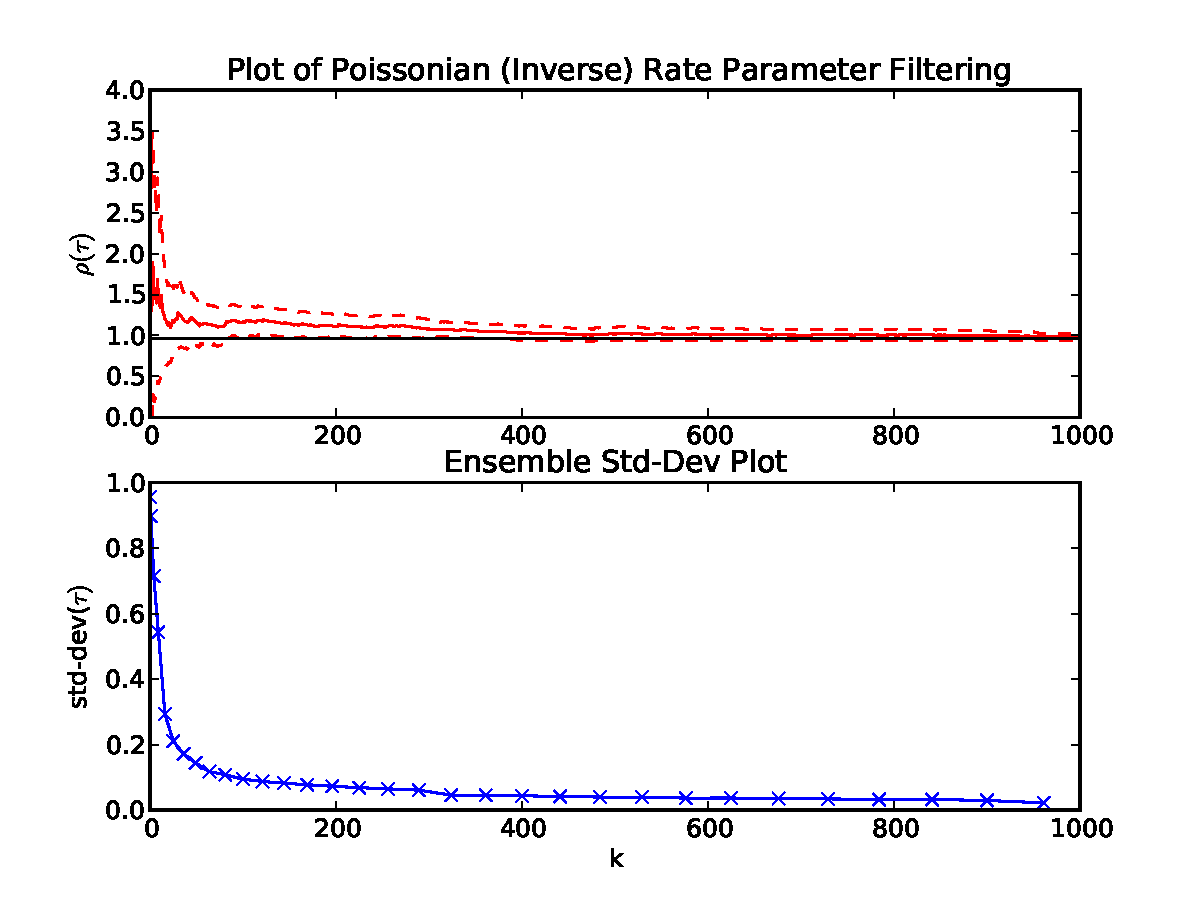
\includegraphics[width=\textwidth]{Figs/TauParticleEnsemble/poisson_rate_filtering.pdf}
%   \caption{Filtering Example for a test-case. We are trying to estimate the
%   inverse of the Poissonian rate, $1/\tau$, given inter-event intervals $t_k$.
%   The true value is $\tau  = 1$. The Maximum Likelihood estimate for $\tau$ in
%   this problem  is just the mean of the observed times $\bar{t_k}$, which
%   happens to be 0.9583 in this example, while after the last observation, the
%   ensemble mean $\pm$ std-dev is $0.9811\pm 0.0199$}
%   \label{fig:poissonian_rate_filtering}
% \end{center}
% \end{figure}

% \clearpage

\subsection{Simulation Results}
We now illustrate how the Optimal Design procedure works while using the
particle filtering methodology to represent and update our parameter prior.

\subsubsection{Single Hitting-Time Illustration}
In \cref{fig:example_online_miopt_single_iteration}, we
illustrate one iteration of the update, that is one hitting time given a
stimulation from either the MI Optimal Controller or from a random controller; the latter 
just gives a randomly chosen constant stimulation for the computation of each hitting time.

Let's discuss what happens in \cref{fig:example_online_miopt_single_iteration}.
Recall that lower values of $\tc$ imply a higher restoring force of the LIF
process towards the origin, and therefore longer hitting times (waiting times).
Since in this sample the observed hitting times were fairly long, especially for
the MI-optimal stimulation, weights for smaller $\t$s grow larger, while weights
for bigger $\t$s become smaller. However it is immediately clear that the
MI-optimal stimulation is more discerning as it has almost entirely discarded
(correctly) the possibility that $\tau>2$, while the other two stimulations have
resulted in only mild perturbations of the prior distribution.

\begin{figure}[h]
\begin{center} 
\subfloat[Particle Ensemble Updates]
{
\label{fig:example_particle_ensemble_updates_for_online_miopt}
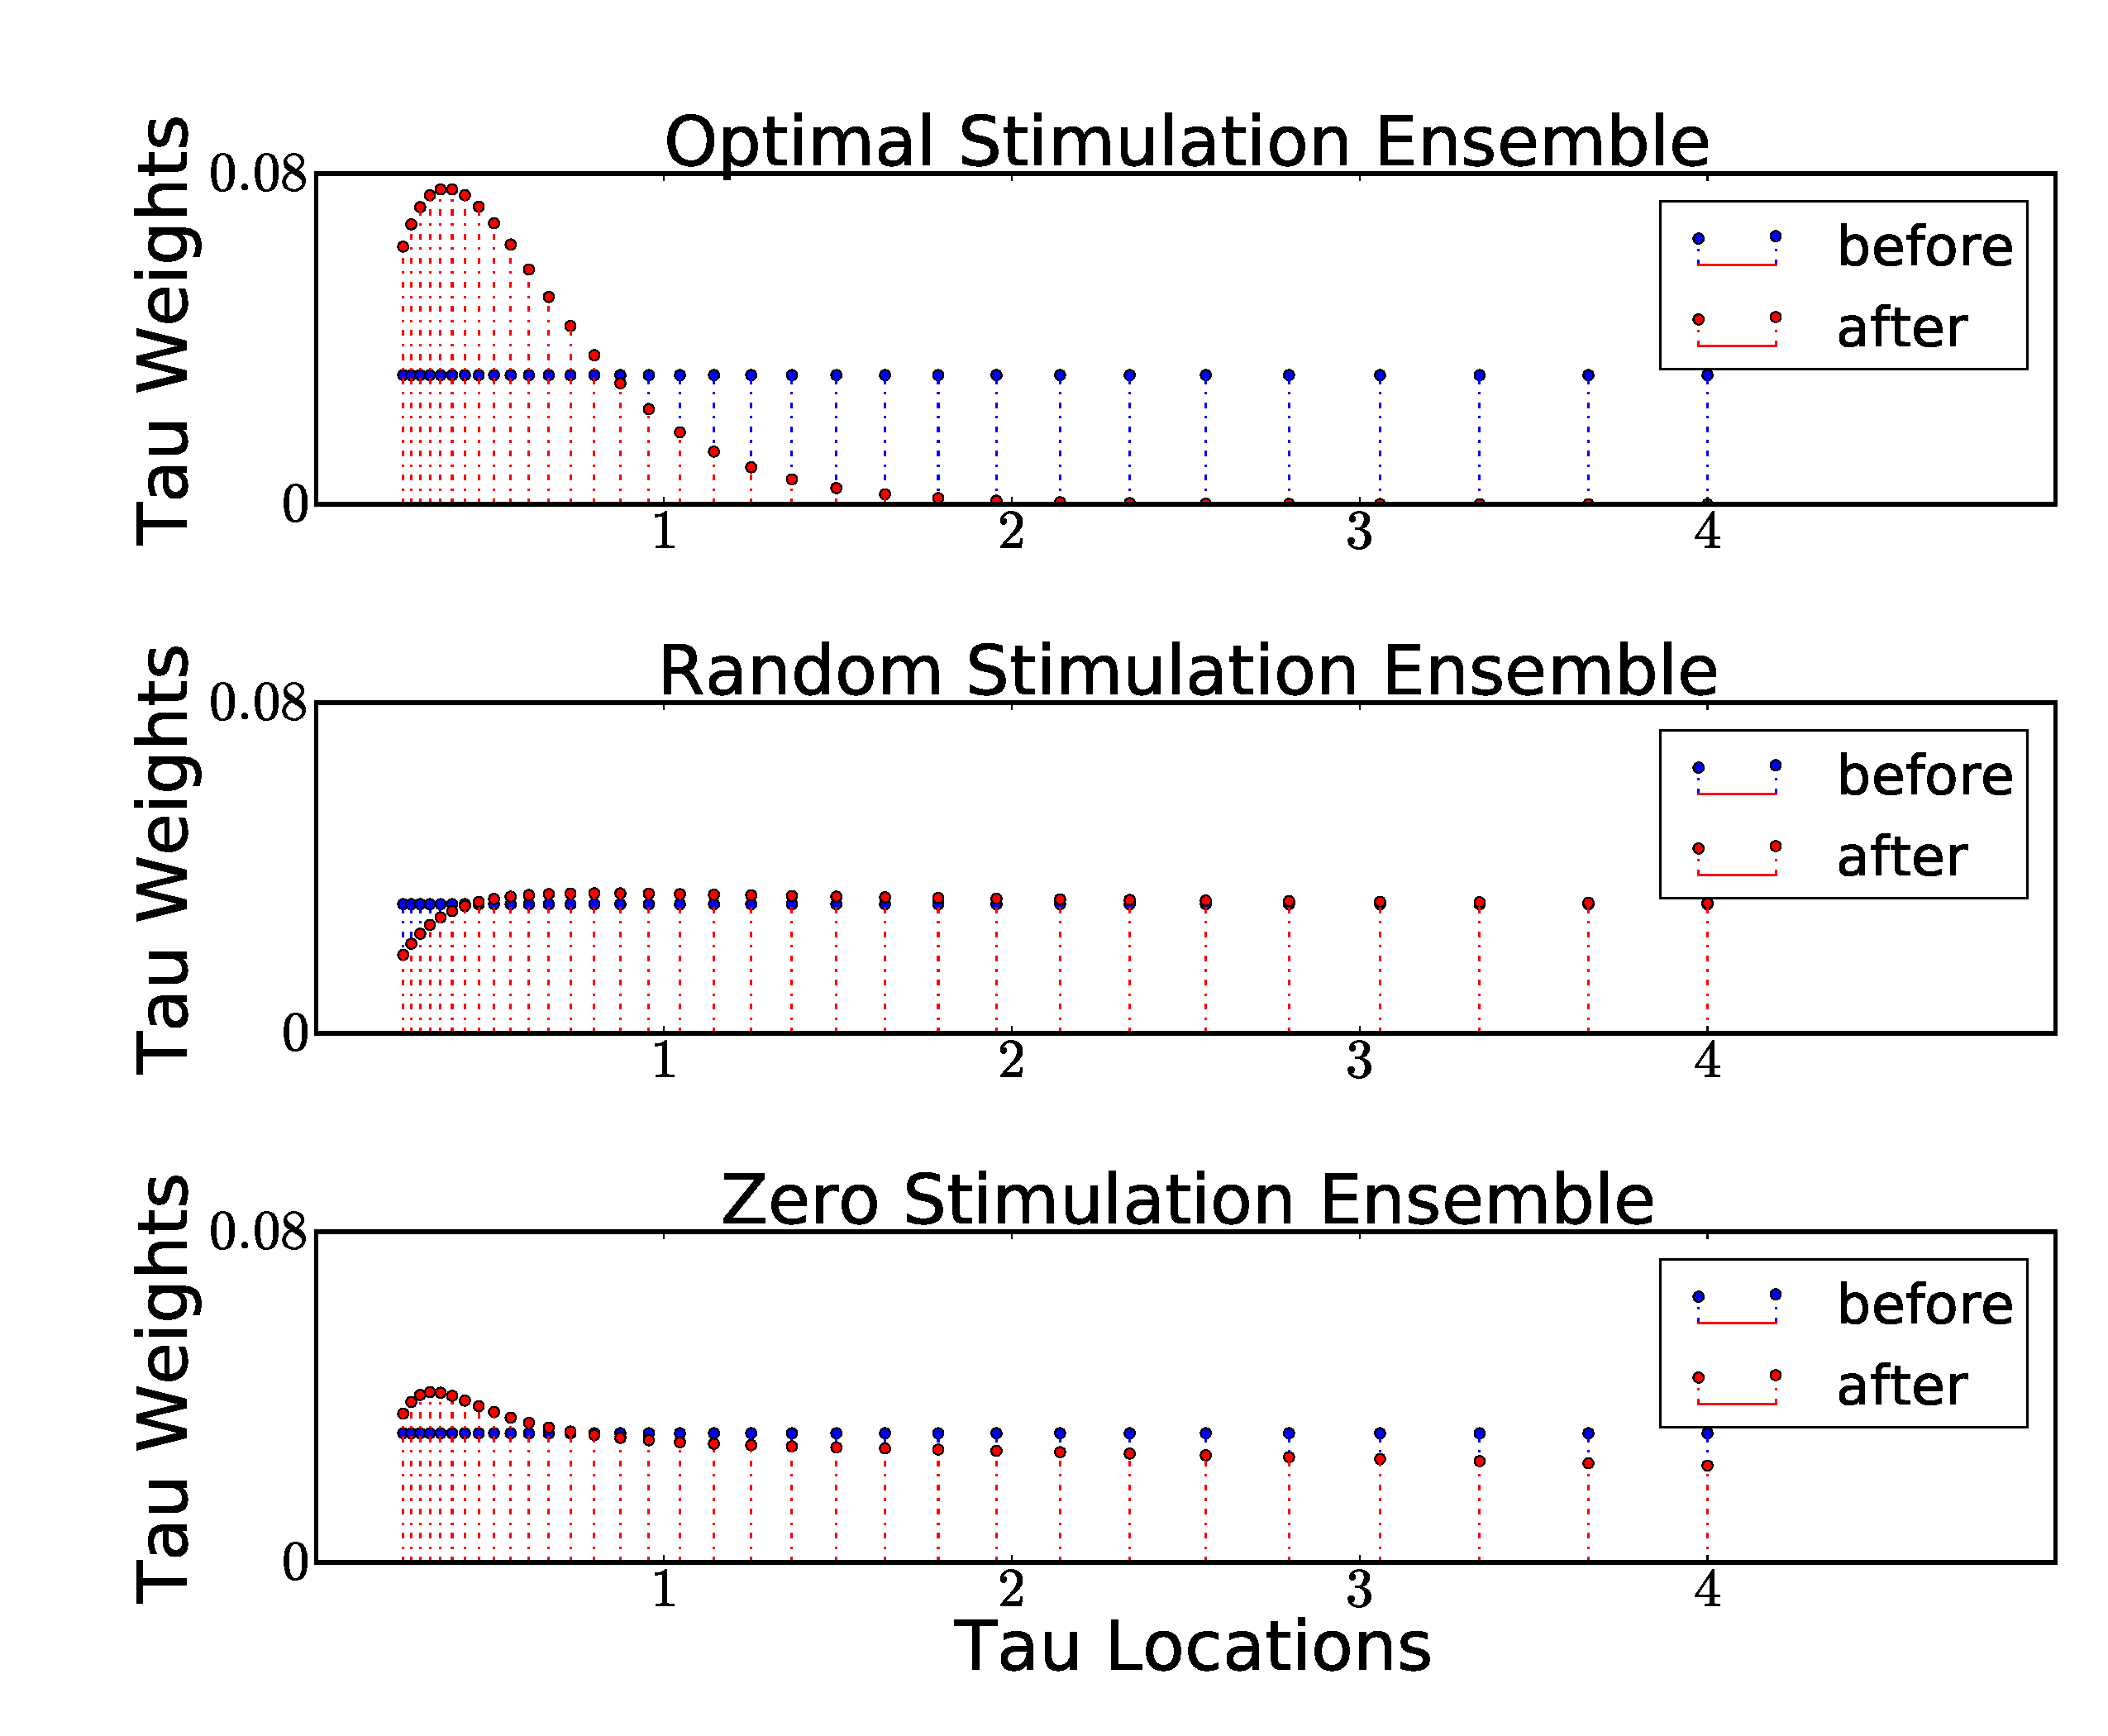
\includegraphics[width=0.80\textwidth]
{Figs/HTOnlineEstimator/single_trial_example_weights.pdf}
}
\caption[Effect of the First Observation on the Belief
Distribution]{Examples of a single iteration of the Online Stimulation-Estimation scheme.
The actual hitting-time observations were 8.16 (optimal stimulation), 1.02
(random stimulation), 7.62 (zero-stimulation) }
\label{fig:example_online_miopt_single_iteration}
\end{center}
\end{figure}  

\subsubsection{Full Multiple Hitting-Times Experiment}
Finally, let us compute an entire estimation experiment. We stimulate a sequence
of hitting times and online update our parameter prior distribution, after
every observation and then online-update our MI-optimal stimulation as the
prior evolves.

% The main result is shown in \cref{fig:example_miopt_vs_rand_ensemble_evolution},
% where we visualize the mean and confidence intervals for the belief
% distributions for the three protocols (MI-Optimal vs. Random Constant vs Zero),
% using $N_\t = 32$ particles and $N_k=251$ hitting times. In
% \cref{fig:example_miopt_controls_evolution}, we show the different stimulations
% that were chosen by the Mutual-Info Maximization Algorithm.
 
% \begin{figure}[htp]
% \begin{center}
%   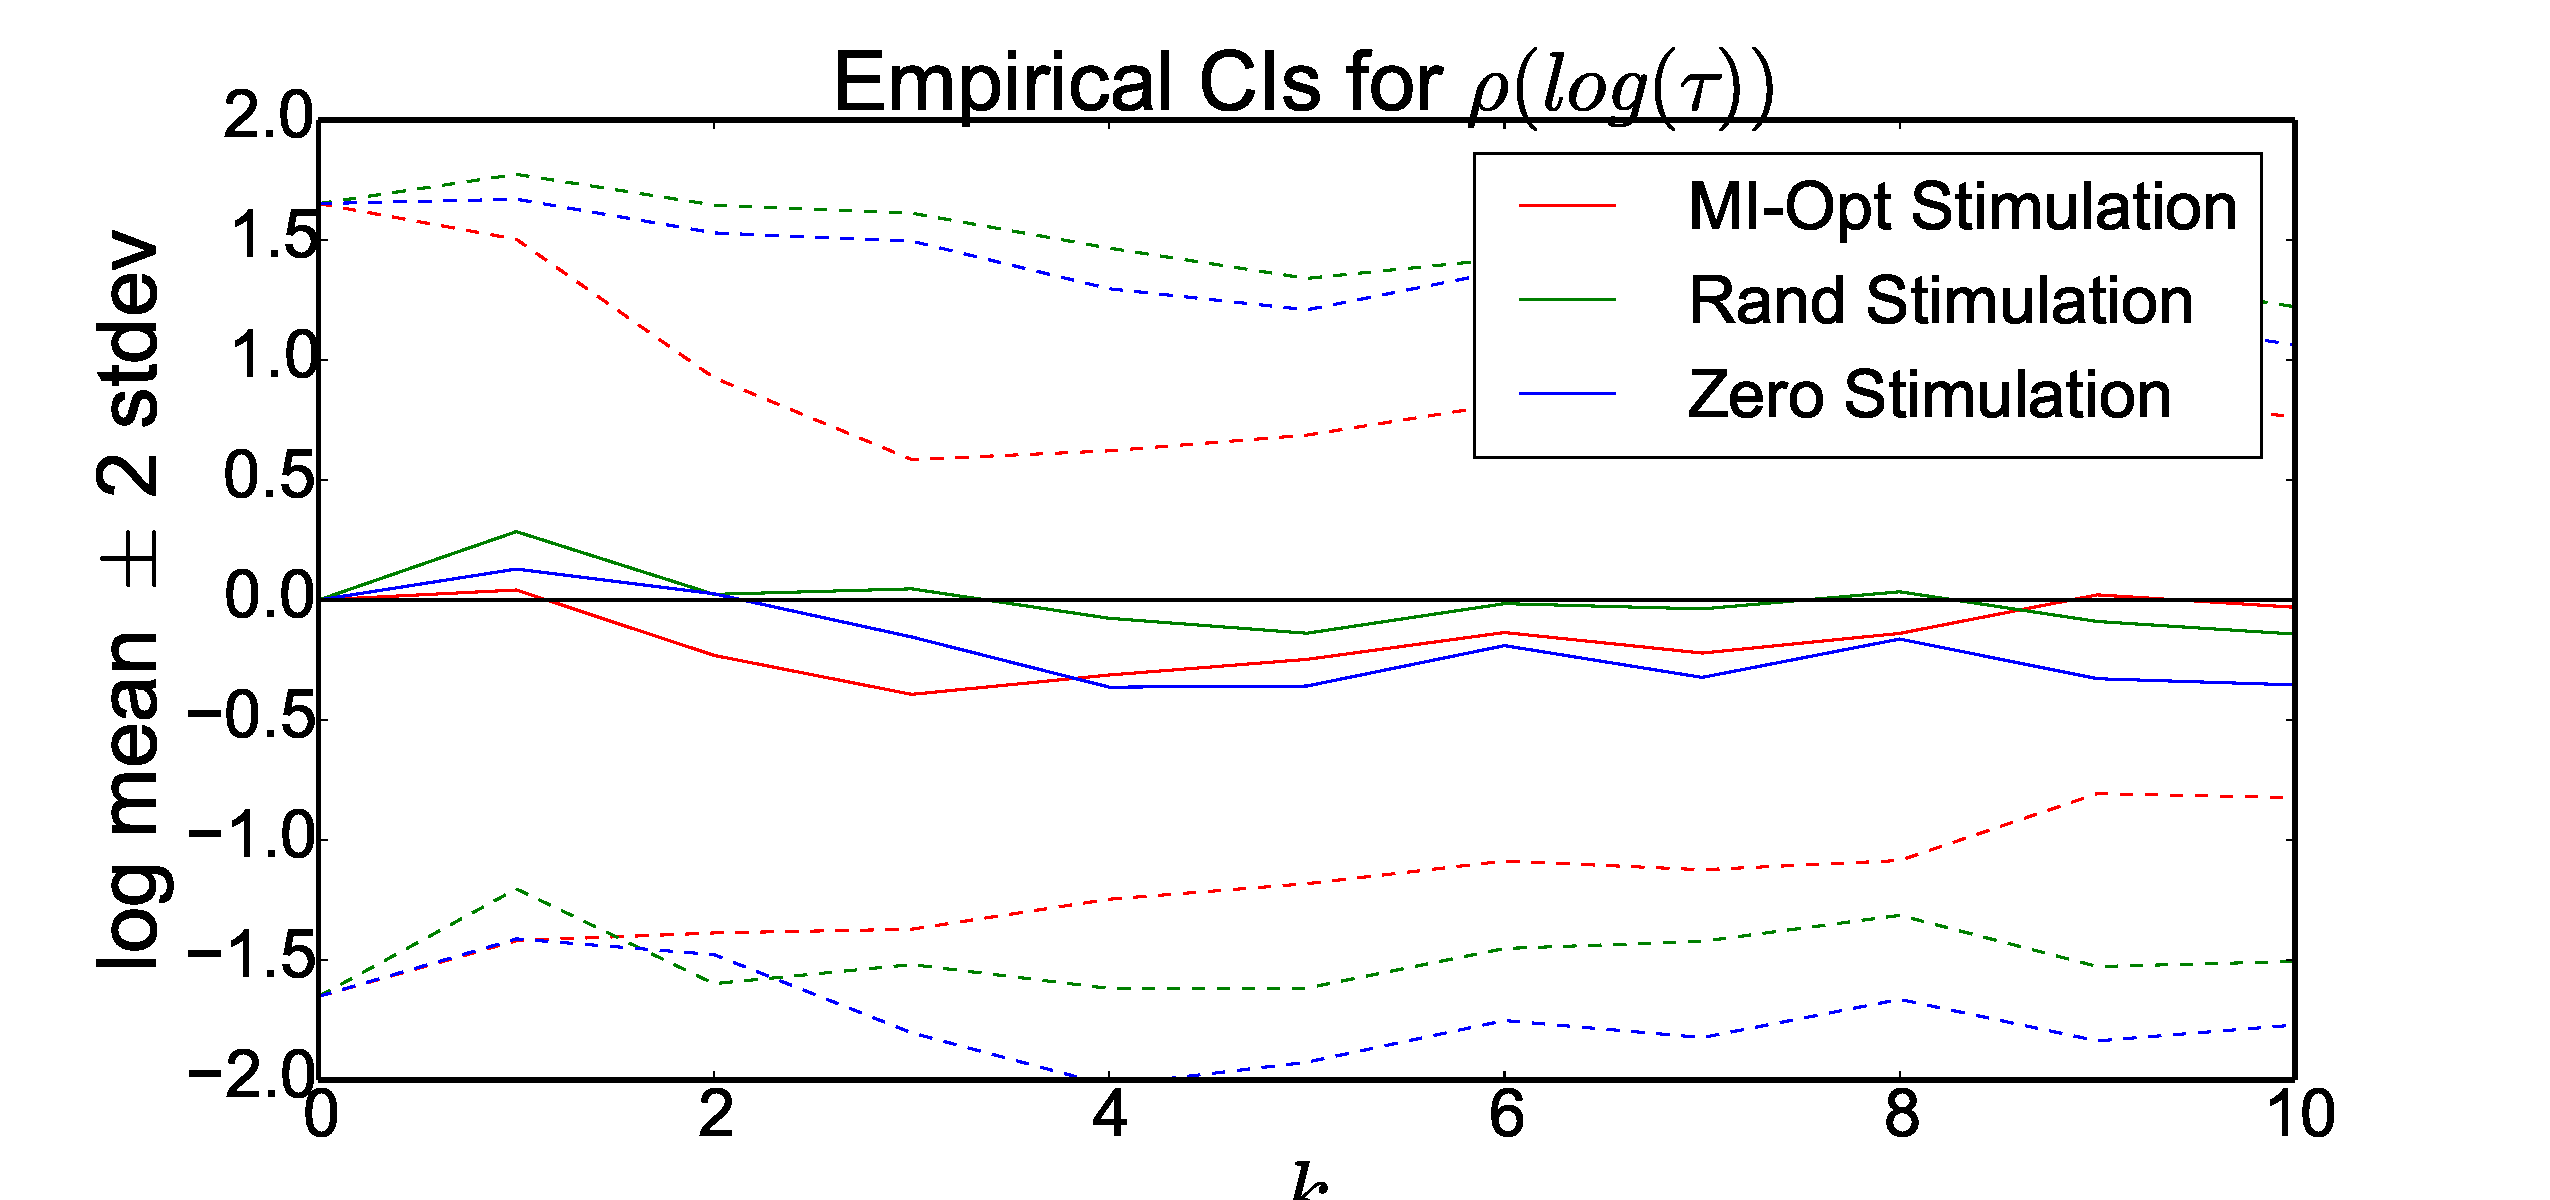
\includegraphics[width=\textwidth]{Figs/HTOnlineEstimator/single_experiment_example_ensemble_distn_evolution.pdf}
%   \caption[labelInTOC]{Evolution of the belief distributions given Optimal
%   (red) or Random (green) stimulation. We used $N=32$ particles to represent
%   the ensemble for both stimulation protocols. There are 250 hitting times used}
%   \label{fig:example_miopt_vs_rand_ensemble_evolution}
% \end{center}
% \end{figure}
% \begin{figure}[htp]
% \begin{center}
%   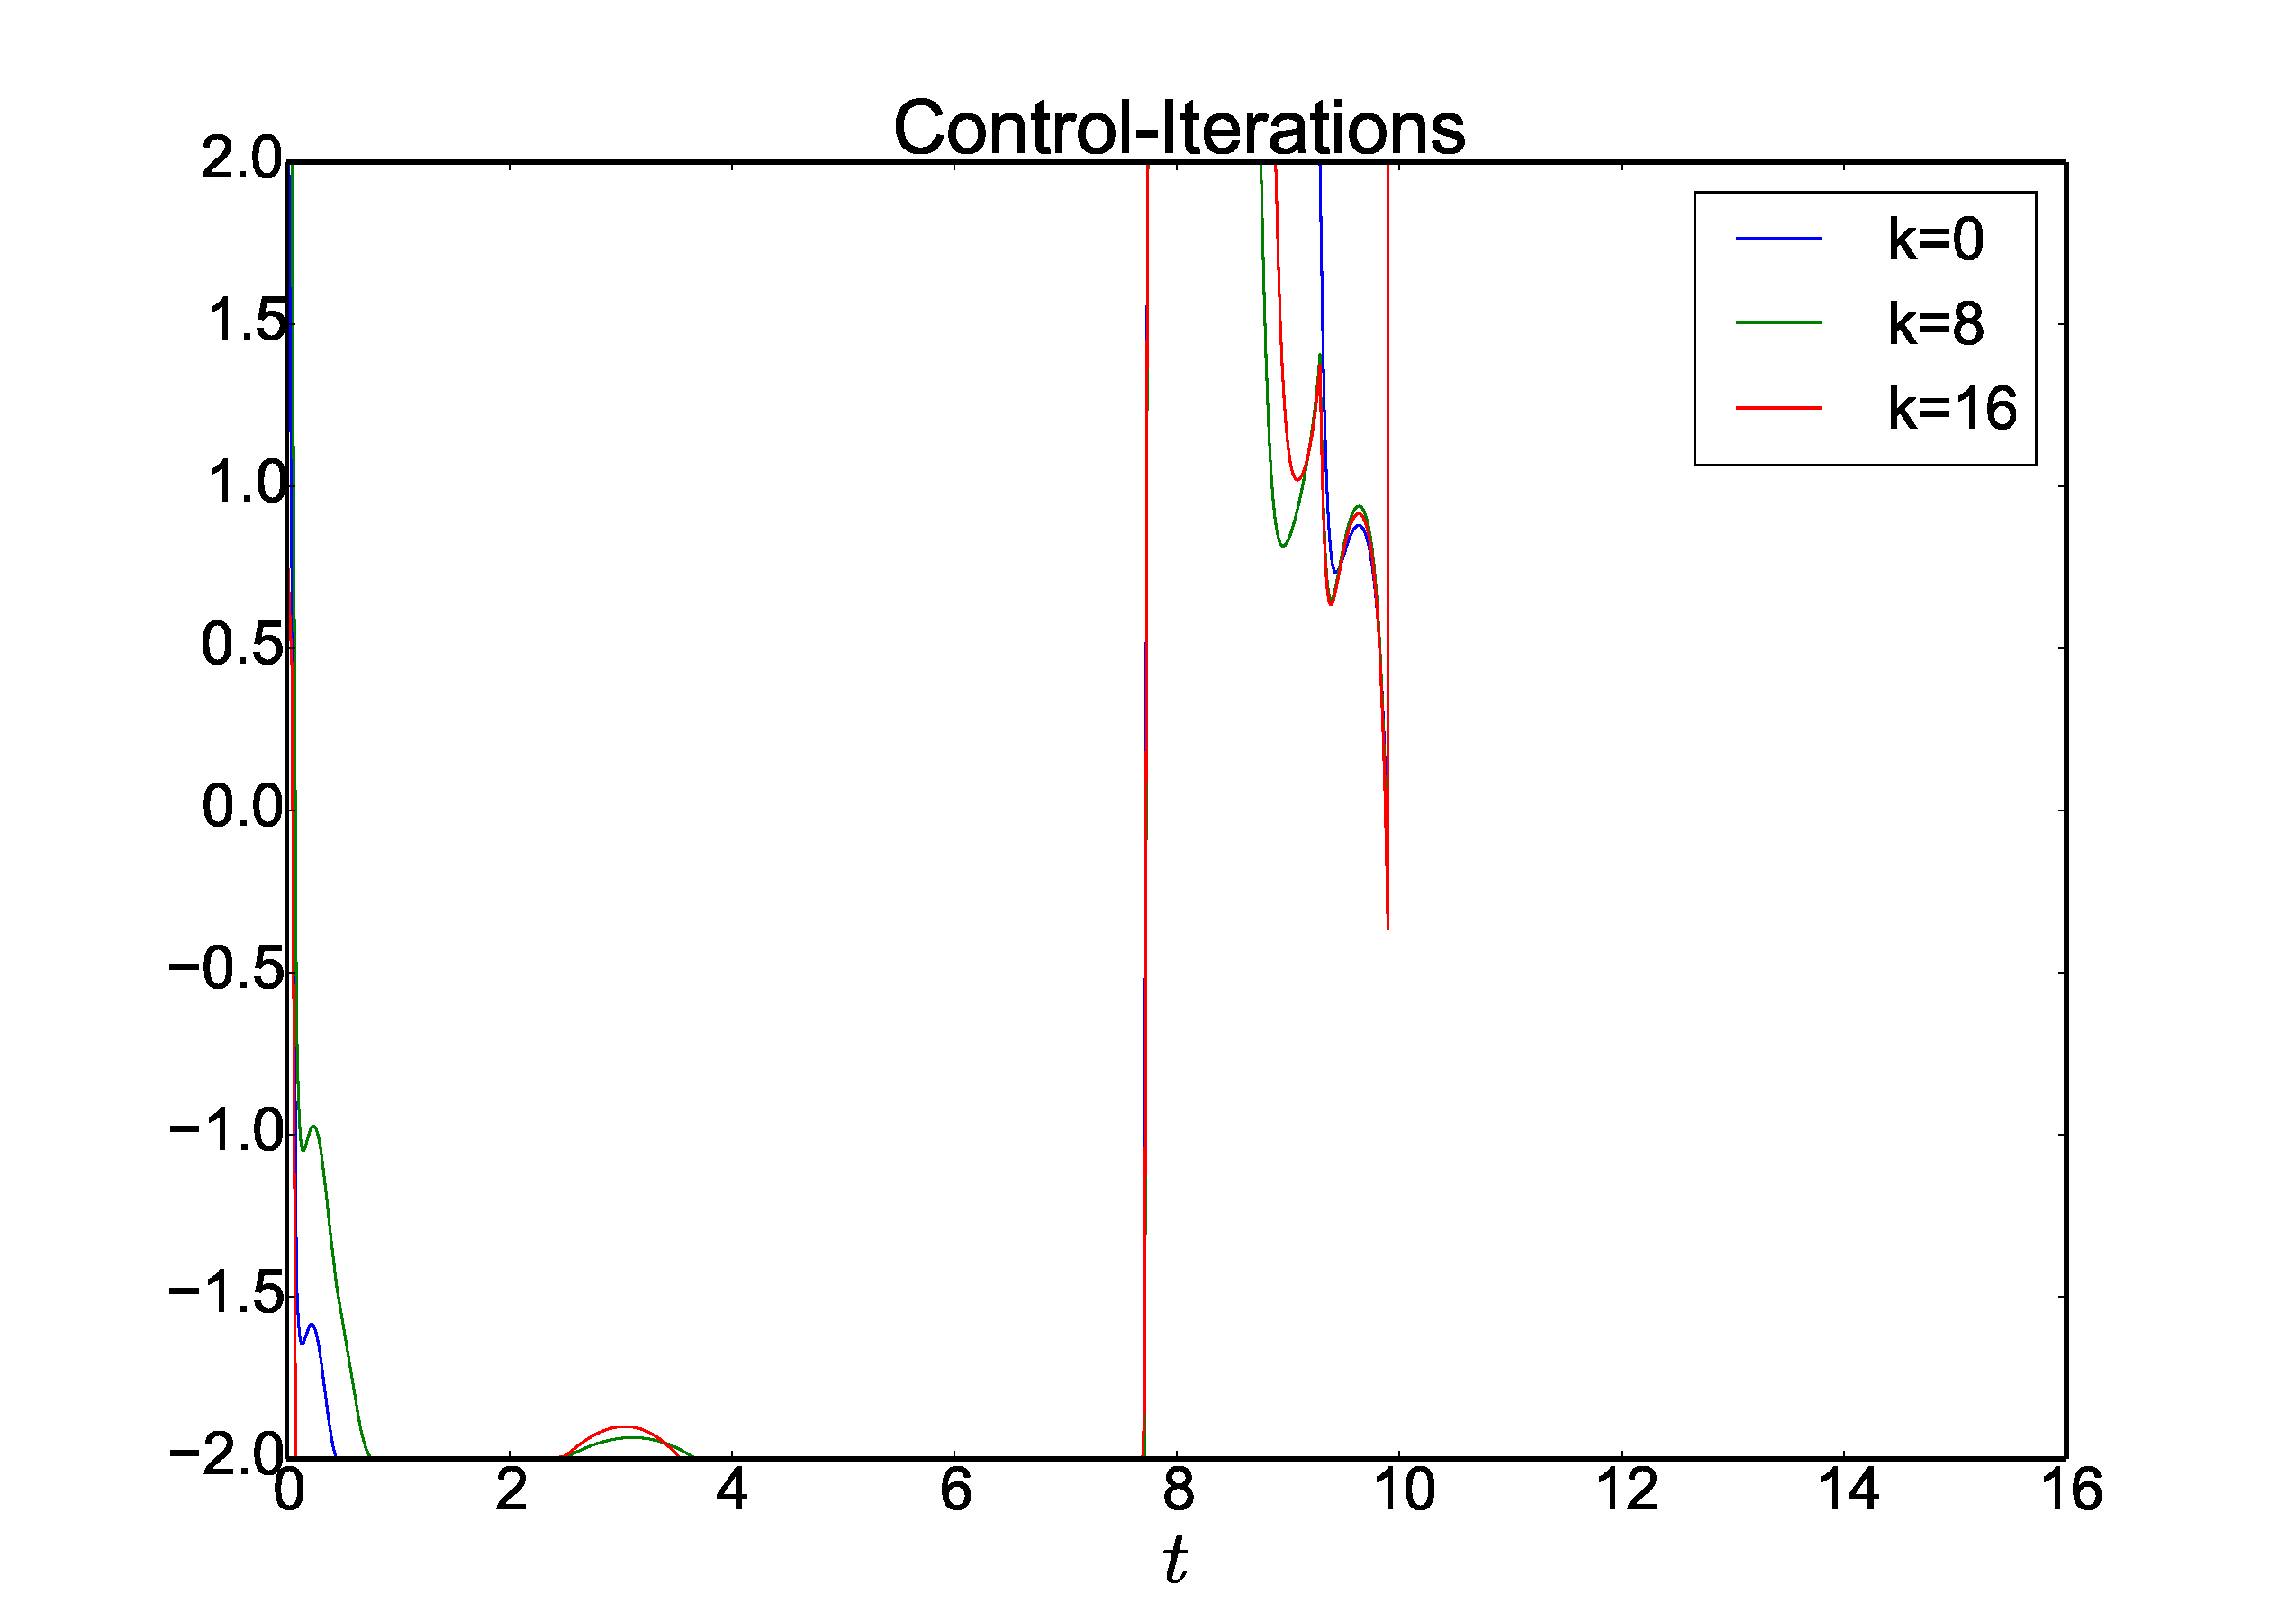
\includegraphics[width=\textwidth]{Figs/HTOnlineEstimator/single_experiment_example_controls_evolution.pdf}
%   \caption[labelInTOC]{Different MI-OPtimal Stimulations computed 
%   as the Experiment evolves and the parameter belief distribution changes}
%   \label{fig:example_miopt_controls_evolution}
% \end{center}
% \end{figure}
 
% \clearpage
 
We now simulate $50$ independent experiments of 500 hitting times each and
then average the ensembles.

% We visualize them in \cref{fig:online_optimization_more_examples}. Here, we
% see that the MI-optimal stimulation is indeed producing more accurate
% estimates, faster (earlier in the experiment). This is true in 7 out of the 10
% experiments, in 2 it is hard to determine whether there is a 'better' protocol
% and only once is the MI-based stimulation resulting in worse estimates than
% one of the alternatives ((f) in \cref{fig:online_optimization_more_examples}).
% \begin{figure}[h] \begin{center} \subfloat[] {
% \includegraphics[width=0.48\textwidth]
% {Figs/HTOnlineEstimator/single_experiment_exampleNts=32_Ntrls=495_ensemble_distn_evolution.pdf}
% } \subfloat[] { \includegraphics[width=0.48\textwidth]
% {Figs/HTOnlineEstimator/single_experiment_exampleNts=32_Ntrls=496_ensemble_distn_evolution.pdf}
% }\\
% \subfloat[] { \includegraphics[width=0.48\textwidth]
% {Figs/HTOnlineEstimator/single_experiment_exampleNts=32_Ntrls=497_ensemble_distn_evolution.pdf}
% } \subfloat[] { \includegraphics[width=0.48\textwidth]
% {Figs/HTOnlineEstimator/single_experiment_exampleNts=32_Ntrls=498_ensemble_distn_evolution.pdf}
% }\\
% \subfloat[] { \includegraphics[width=0.48\textwidth]
% {Figs/HTOnlineEstimator/single_experiment_exampleNts=32_Ntrls=499_ensemble_distn_evolution.pdf}
% } \subfloat[] { \includegraphics[width=0.48\textwidth]
% {Figs/HTOnlineEstimator/single_experiment_exampleNts=32_Ntrls=500_ensemble_distn_evolution.pdf}
% }\\
% \subfloat[] { \includegraphics[width=0.48\textwidth]
% {Figs/HTOnlineEstimator/single_experiment_exampleNts=32_Ntrls=501_ensemble_distn_evolution.pdf}
% } \subfloat[] { \includegraphics[width=0.48\textwidth]
% {Figs/HTOnlineEstimator/single_experiment_exampleNts=32_Ntrls=502_ensemble_distn_evolution.pdf}
% }\\
% \subfloat[] { \includegraphics[width=0.48\textwidth]
% {Figs/HTOnlineEstimator/single_experiment_exampleNts=32_Ntrls=503_ensemble_distn_evolution.pdf}
% } \subfloat[] { \includegraphics[width=0.48\textwidth]
% {Figs/HTOnlineEstimator/single_experiment_exampleNts=32_Ntrls=504_ensemble_distn_evolution.pdf}
% } \caption[labelInTOC]{Various examples of the perturbation-estimation
% protocol with the belief distribution plotted against the hitting time $k$,
% with the MI-optimal stimulation (red), the constant random stimulation (green)
% and the zero, $\a\equiv 0\,\forall t$, stimulation (blue)}
% \label{fig:online_optimization_more_examples} \end{center} \end{figure}
The aggregated evolutions for the updated prior distributions are
visualized in \cref{fig:online_optimization_aggregated_belief_evolution}. It is now clear that
the MI-Optimal procedure produces more accurate and more precise estimates and
that the increase in precision is especially clear in the earlier parts in the
experiment. That is, using the MI-optimal protocol reduces the uncertainty in
the parameters much faster.

In \cref{fig:online_optimization_quantiles_belief_evolution}, we plot the
quantiles of the running means of the updated priors for the  $N$
experiments. We see a similar behaviour as in
\cref{fig:online_optimization_aggregated_belief_evolution}, such that the
optimally stimulated prior converge to the true value and have much lower
uncertainty around it, while the base cases are neither not accurate nor
particularly precise, which is consistent with the general 
 
 
% \usepackage{graphics} is needed for \includegraphics
\begin{figure}[htp]
\begin{center}
  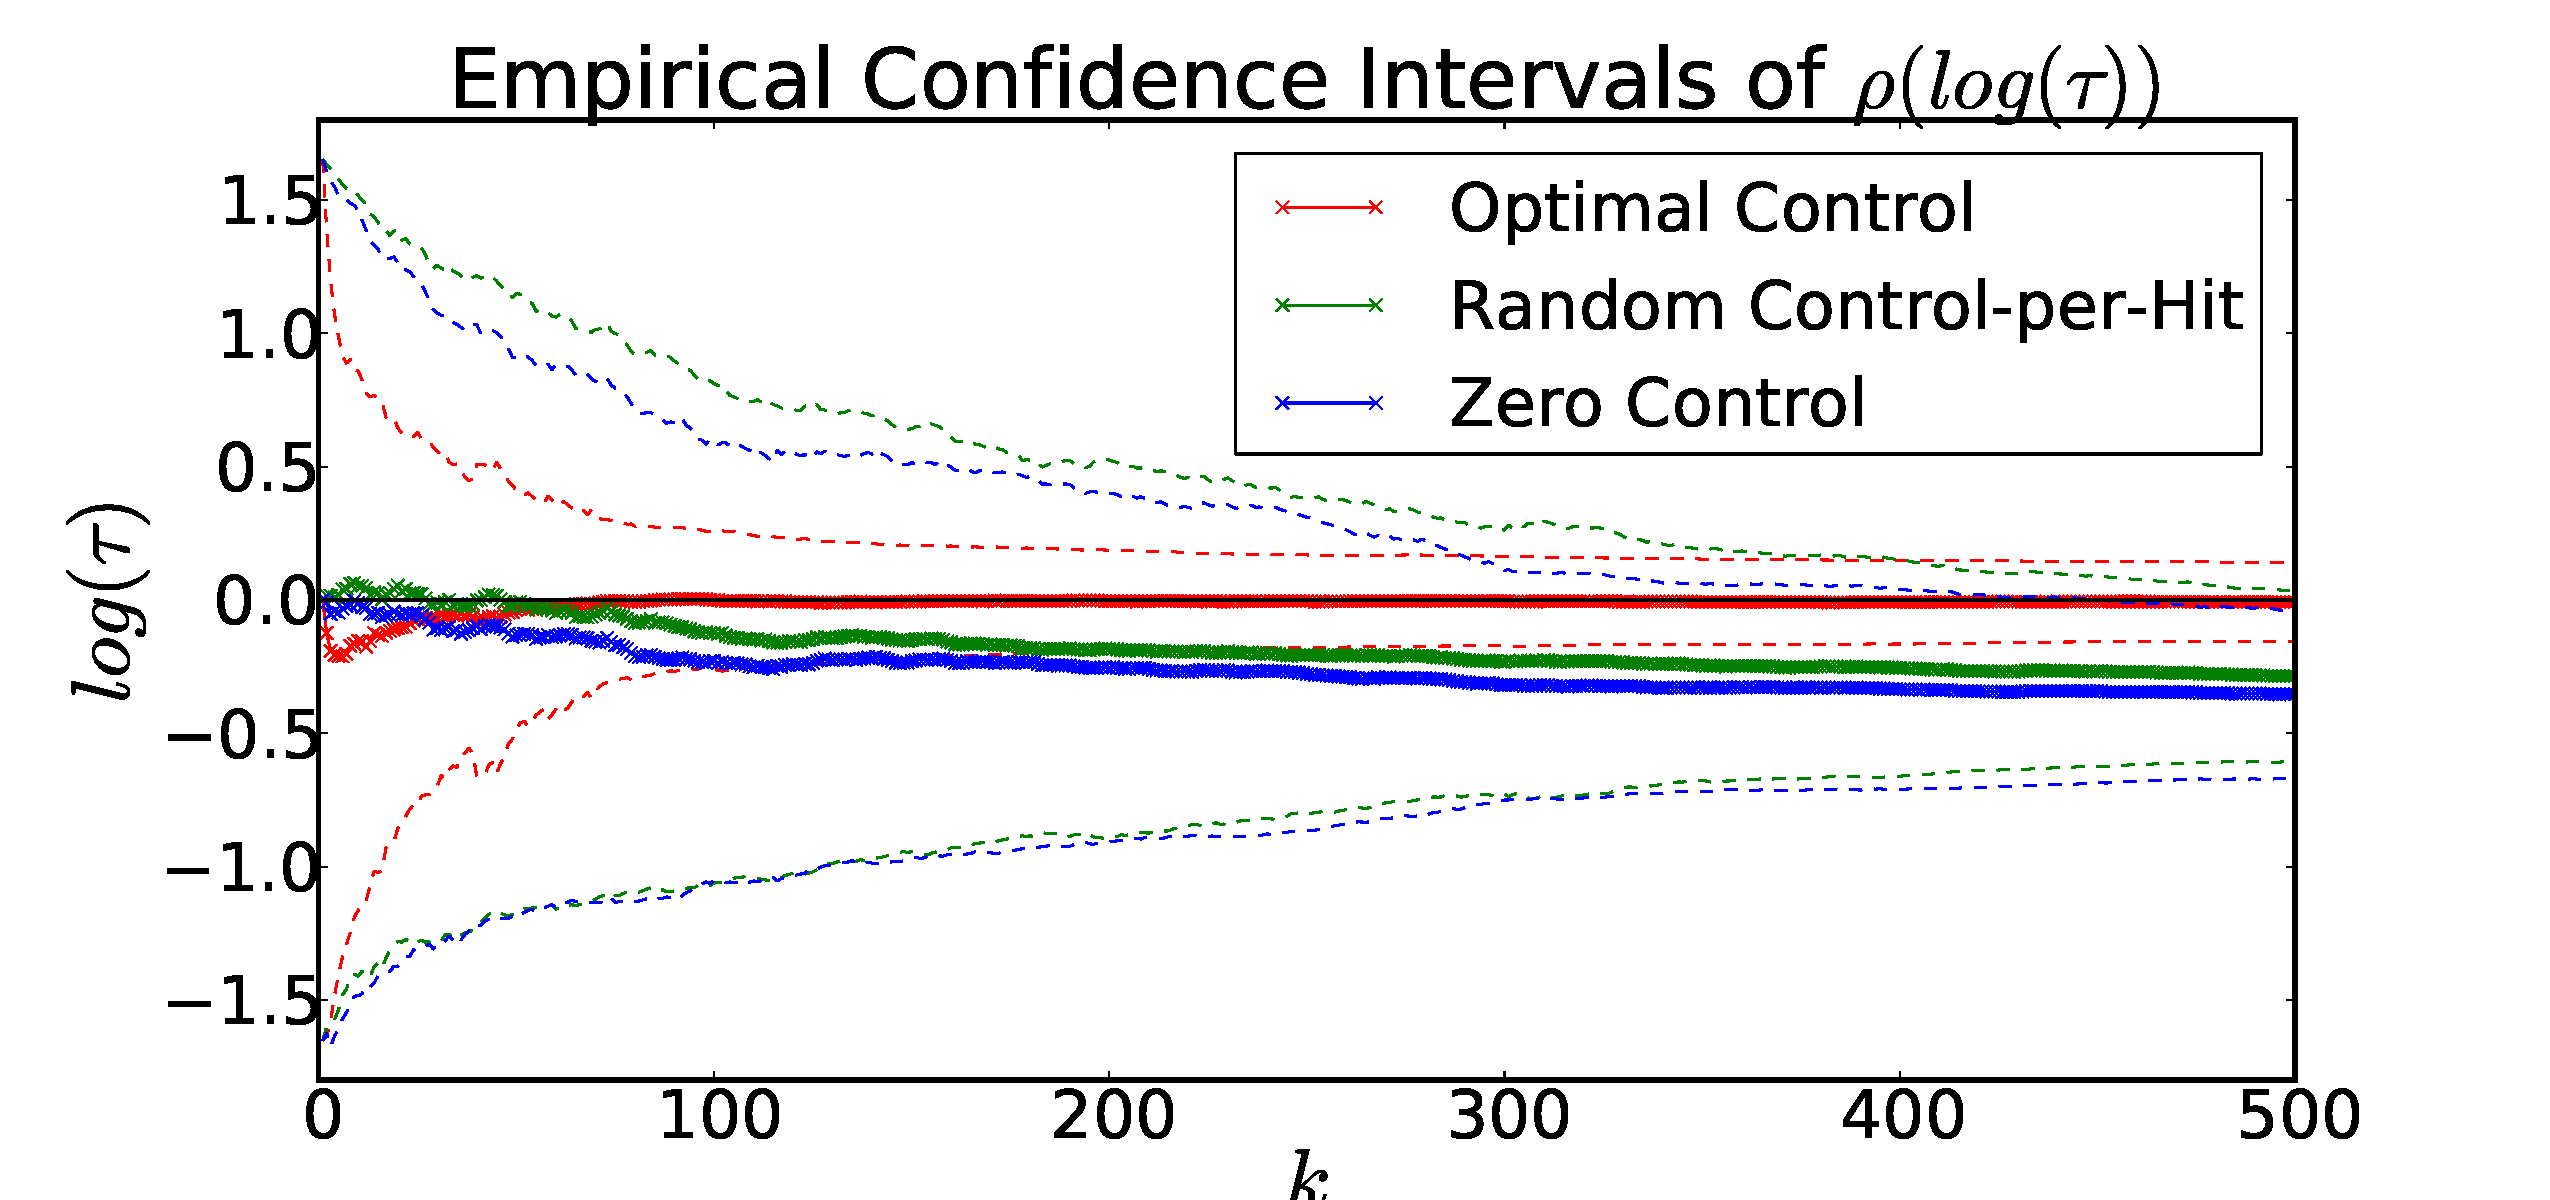
\includegraphics[width=\textwidth]{Figs/HTOnlineEstimator/online_updated_prior_mean_aggregated_ensemble.pdf}
  \caption[Optimal Stimulation produces more precise parameter estimates]
  {Optimal-designed stimulation produces more precise and more accurate
  parameter estimates. 
  Visualized are the mean and confidence intervals for the parameter
  distribution of $\log (\tau)$, averaged over $N=50$ independent
  experiments. The black line indicates the 'true' value of the log of the
  unknown parameter $\tau$ used to generate the
  synthetic observations. 
  The solid (red,green and blue) lines indicate the mean of
  $\rho_{k, avg}(\log(\t)))$, while the dashed lines indicates 2 standard
  deviations in either direction of the mean. 
  The averaged prior is obtained by taking the $N$ individual priors after the
  $k$th hitting times, $\rho_{j,k}(\log(\tau)))$ and averaging them (i.e. it is
  an equally weighted mixture of the $N$ individual densities.
Clearly, we see that the mean and the plus/minus 2 standard deviations of the 
stimulated estimates are much closer to the true value of the parameter,
$\log(\tau)$ then the estimates obtained from the naive stimulations.}
  \label{fig:online_optimization_aggregated_belief_evolution}
\end{center}
\end{figure}
%\usepackage{graphics} is needed for \includegraphics
\begin{figure}[htp]
\begin{center}
  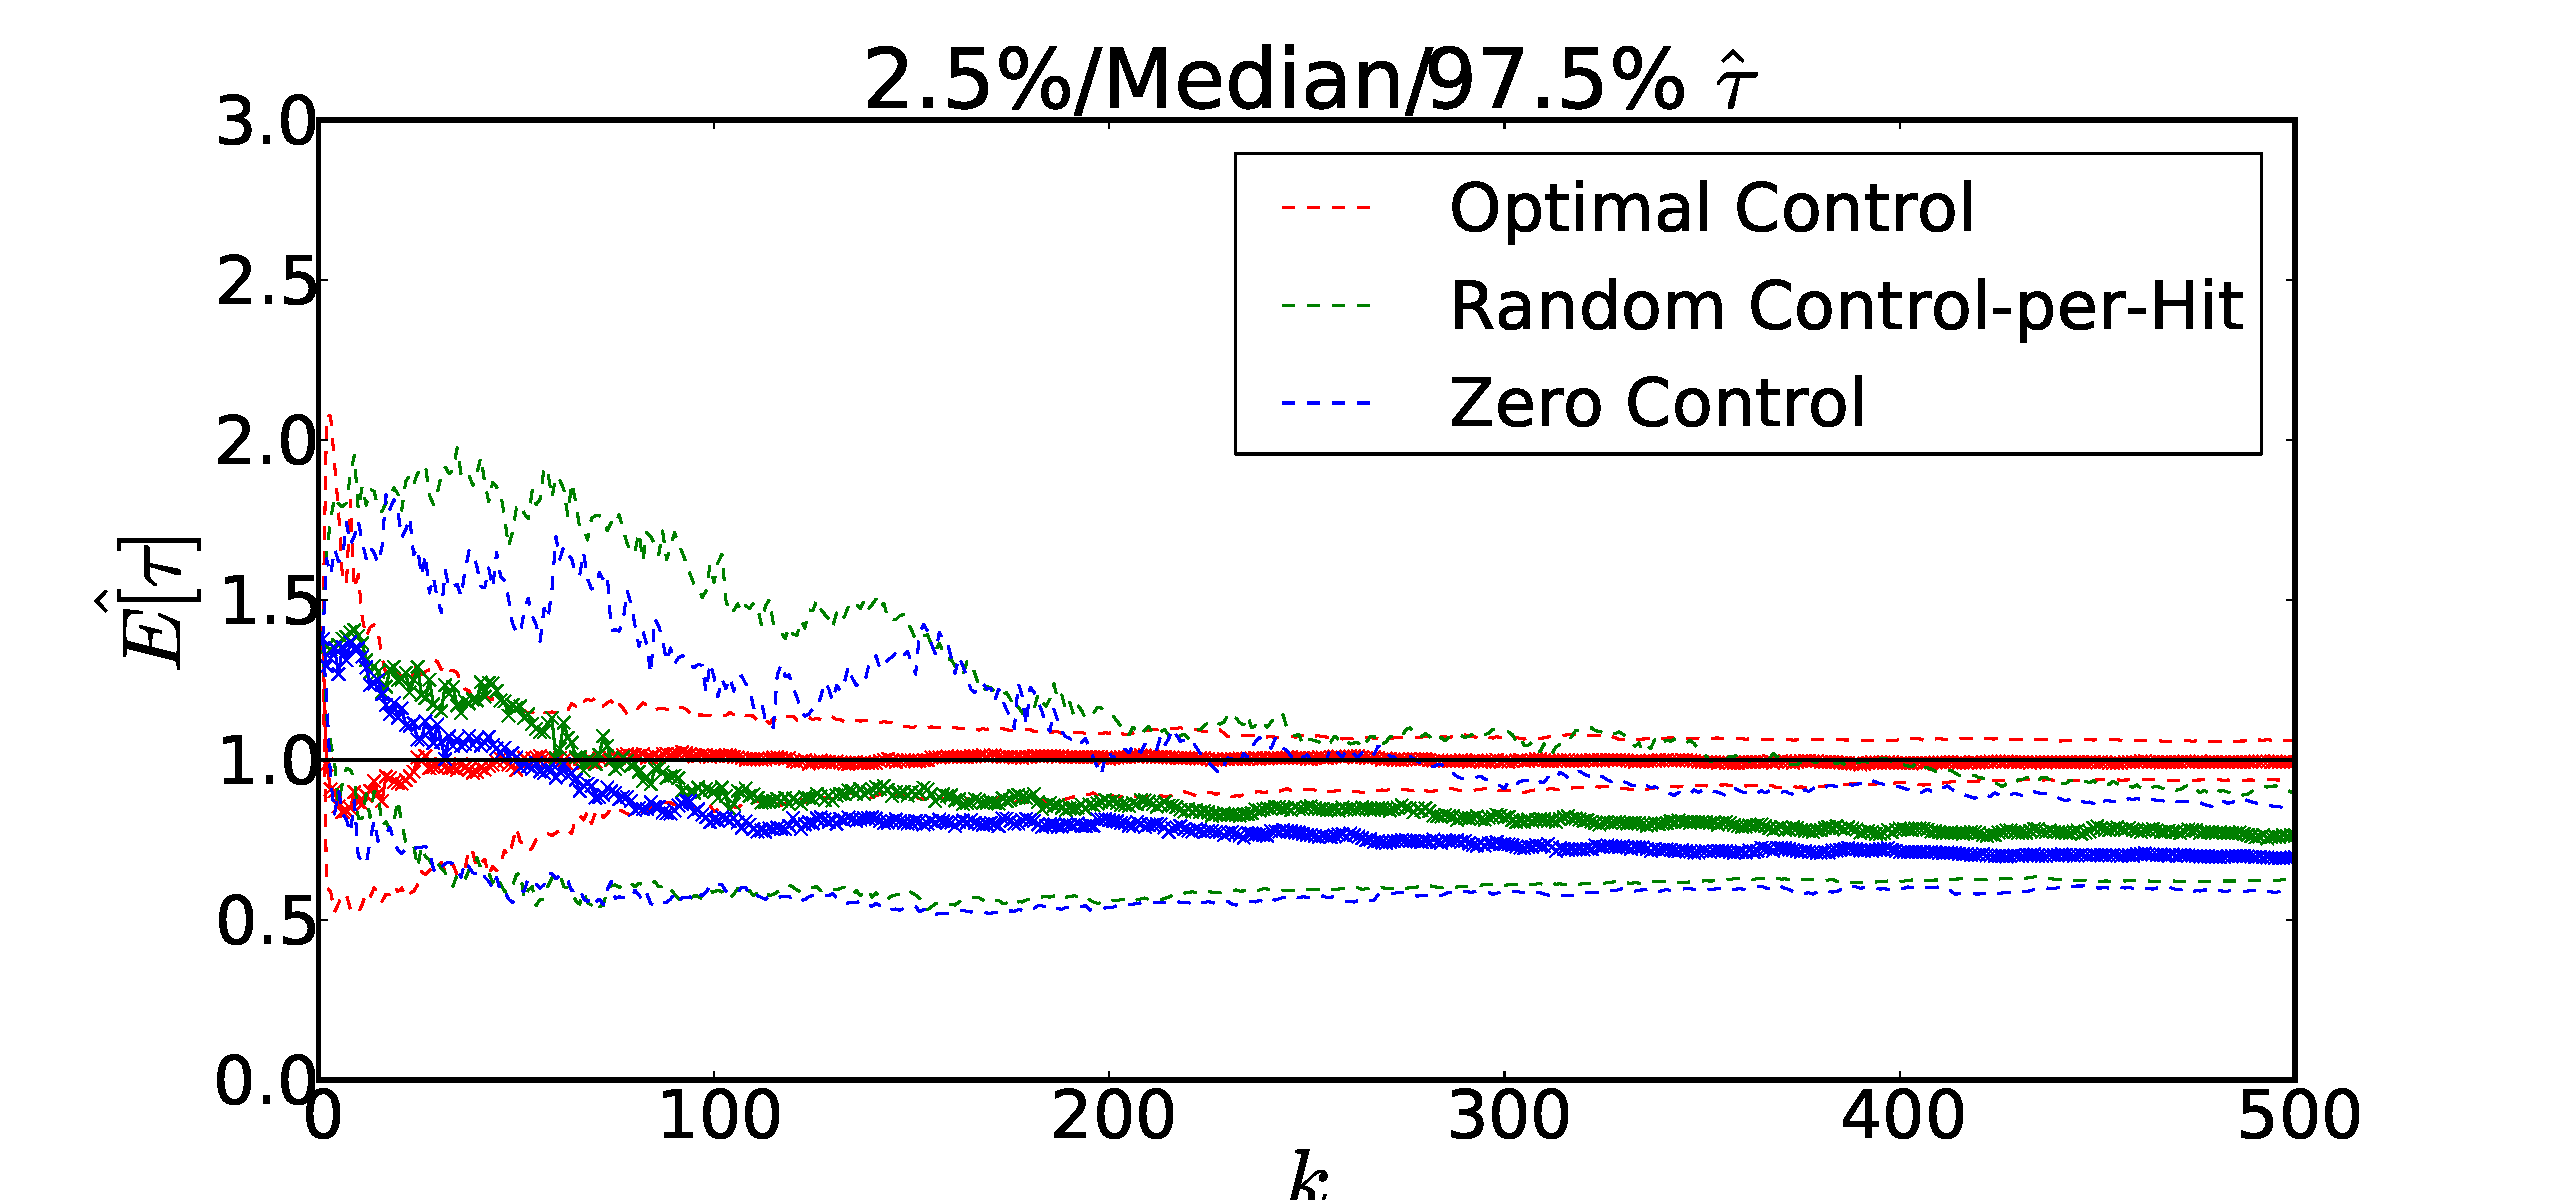
\includegraphics[width=\textwidth]{Figs/HTOnlineEstimator/online_updated_prior_quantiles_mean_per_experiment.pdf}
  \caption[Quantiles of the Mean Estimates]{Optimal-designed stimulation produces more precise and more accurate
  parameter estimates. 
  Visualized are the median and
  2.5/97.5th percentiles of the mean of the updated prior
  distribution over the $N=50$ experiments. I.e.\ for each experiment, $j$, and
  each hitting time, $k$, we compute the mean of the updated prior $\rho_{j,k}(\tc)$
  and then we plot the median (crosses) of these $N$ means as well as the second
  smallest and second-largest of them (dashes). 
  The black line indicates the true value of $\tau$ used to generate the
  synthetic observations. 
  Again we see that the median and the extreme quantiles of the
  optimally stimulated estimates are much closer to the true value of the parameter, $\tau$ then the estimates obtained from the naive stimulations.}
  \label{fig:online_optimization_quantiles_belief_evolution}
\end{center}
\end{figure}

\section{Discussion}
\label{sec:discussion}
We introduced a method for optimal design given hitting-time observations. This
contrasts with earlier work where the control is based on observations of the
state variable of the stochastic differential equation whose parameters are to
be estimated. Our method is based on maximizing the Mutual Information between
the observed hitting times and the posterior distribution of the parameters. The
optimal control tends to separate the hitting-time distributions associated with
alternative values of the unknown parameter, thereby facilitating the
identification of the parameter once an observation is made. The simulations
show that the resulting estimates from the optimally-stimulated system have
higher precision and accuracy than sensible alternatives, such as random
stimulation, 'critical' stimulation at $\alpha=\xth/\tc$, or no stimulation at
all.

% (ALEX: ADD A WORD ABOUT THE MATH ADVANCE, I.E. a technical sentence or two on
% how you put in the hitting time to the design problem)
Since the Mutual Information is expressed in terms of the hitting-time density
and the hitting-time density can be related to the boundary term of a
Fokker-Planck PDE, we approach the maximization of the Mutual Information as a
PDE optimization problem. The standard use of an adjoint variable to obtain the
objective gradient is made more complicated by the outer integration with
respect to the unknown parameter prior. However we are still able to derive the
adjoint PDEs and thus to compute the objective gradient despite this added
complication.
 
% ALEX: SAY WHY IT CAN BE EXPENSIVE AND WHAT CAN BE DONE TO MINIMIZE THIS COST -
% maybe a word about the dependence of cost on number of particles - since you
% said it relates to number of PDE's)
Our PDE-based adjoint optimization methods can be expensive and sensitive to the
various parameters of the optimization. The main computational cost is the
numerical solution to the forward and backward PDEs, which have to be solved
numerous times during the optimization search. In principles one has to solve as
many PDEs as there are particles in the prior distribution. However, we have
seen that in practice it is sufficient to use very coarse approximations to the
prior. For example as few as two or three particles which match the
mean/variance of the more detailed higher-resolution prior seem to be sufficient
to obtain the same optimal control as that obtained by using all the particles
in the prior, at least for our problem.
 
In general, the optimally-stimulated samples give (much) more accurate estimates
than the ones that are naively-stimulated. However, we see in
\cref{fig:beta_estimates_from_hitting_times_different_alphas}, panel b) that
occasionally (once), the optimally-stimulated sample can give very wrong
estimates. We have taken a closer look at what happens in those situations. 
It seems that in the bad cases, there are enough extreme (i.e. very long)
hitting times that the estimation procedure infers a very small characteristic
time (i.e the attractive force towards $\mu=0$ is very strong). Generally in
long samples such extreme hitting times are relatively rare, and the correct
parameter value is inferred.

Our results point to a novel way to estimate the characteristic time of the LIF
process. Parameter estimation techniques applied to the hitting this process
have reported difficulties for this particular parameter. This is unfortunate
given that it is a parameter that is deemed important to understand the
integrative properties of single neurons. It is also a parameter that can vary
based on the amount of inputs the neuron receives from other cells; more
specifically it reflects the ongoing conductance of the cell. It would be
particularly interesting to see whether the batch or online implementations of
the hitting-time based optimal design method could be implemented in an
experimental setting and what new challenges arise in this context. Our method
has the advantage of dealing with the intrinsic stochasticity of the underlying
process for designing stimulation protocols that best reveal system parameters.
 
% ALEX: A word about batch vs online
Doing a batch estimation, when the control is computed only once and then
applied for all observations is the computationally simpler approach. More
interestingly, we show that the optimal control can be evolved online as
new observations are assimilated into the parameter prior, and the optimal
control is updated accordingly. However we note that the optimal control is
fairly similar for a wide range of priors, which somewhat limits the
additional value of recomputing the optimal control as the observations from
the experiment are recorded.

% ALEX: A word about figuring out good priors, which are important in particular
% for computation time. remind reader what the opt-narrow vs opt-wide comparison
% yielded.   
In line with the observation that the optimal control is fairly similar for
various priors of $\tau$, we note that the slight differences in the actually
obtained stimulation does not make a big difference when it comes to estimating
the parameters. We note that independent of the prior used, the resulting
estimates in all cases are much better, more accurate and precise, then the
estimates obtained using the base case of no stimulation. 

% ALEX: A word about estimating one or many parameters.
In fact, we empirically demonstrate that our optimal stimulation scheme also
results in excellent estimation results for {\sl all} system parameters, even
though it is designed only to estimate the $\tau$ one.

In general, we note that the control shape that consist of an initial segment
that inhibits spiking, $\a(t) \approx \amin$, followed by a segment that
promotes spiking, where $\a(t) \approx \amax$, is obtained for a wide variety of
priors or model parameters, $\m, \s$. Thus it is natural to conjecture that for
our problem in general, the optimal stimulation has this shape. It is however an
open problem to prove this mathematically.

% ALEX: Add a simple outlook statement in 1-2 sentences about future work.
As future work, we also leave out the work when all the parameters are treated
in the full Bayesian way and the parameter prior is over all of them, not just
over $\tau$. In principle our derivations carry over unchanged,
the only complication is that the prior will need to contain more points to fully
describe the uncertainty in all three. 

Other minor tweaks involve using a more sophisticated gradient optimization
method, such as a nonlinear conjugate gradient, which might be more
computationally efficient. 

Our work can be viewed as an optimal design for 
parameter estimation of PDEs. It would be interesting to see whether in general
the Mutual Information criterion can be applied successfully for the selection of
perturbation in other such PDE parameter estimation contexts. 

\clearpage
\appendix
\section{Mutual Information}
\label{sec:mutual_info_defn} 
The mutual information, $I$, between two random
variables $X$ and $Y$ is defined by
\begin{equation} 
I(X,Y) = \int_{\mathcal{Y}} \int_{\mathcal{X}} p(x,y) \log \frac{p(x,y)}{p(x)p(y)} \intd{x}\intd{y}
\label{eq:mutual_info_defn}
\end{equation}
where $p(\cdot)$ are density functions of their arguments, 
see e.g. \cite{MacKay2003,Cover2006}. Intuitively, it measures the
average reduction in uncertainty about one of the variables by the
knowledge of the other variable, and it is zero if and only if the two
variables are independent.

Here we show that \cref{eq:J_mutual_info_objective} is the mutual
information between the random variables $T_{sp}$ and $\Theta$.  
The marginal distribution of $\Theta$ is simply the prior, $p(\th) =
\rho(\th).$ The joint distribution is $p(t,\th) = 
g(t|\th)\rho(\th)$ by Bayes formula. The marginal of $T_{sp}$ is $p(t) =
\int_\Theta g(t|\th)\rho(\th) \intd{\th}$. 
Plugging the three expressions into the definition in
\cref{eq:mutual_info_defn} yields
\begin{equation}
I = \int_\Theta \int_0^{\infty} g(t|\th)\rho(\th) 
\log \left( \frac{g(t|\th)\rho(\th) }{\rho(\th)\int_\Theta g(t|\th)\rho(\th) \intd{\th}
 } \right)
\intd{t}\intd{\th}.
\label{eq:mutual_info_prior_trajectory}
\end{equation}
After canceling $\rho(\th)$ inside the $\log$, we get
\cref{eq:J_mutual_info_objective} .

\clearpage

\section{Numerical Algorithms}
\begin{algorithm}
\begin{algorithmic}
\caption{Gradient ascent algorithm for obtaining the optimal control.
The objective gradient with respect to the control is computed up to $K_{max}$
times and at each iteration $k$, the $k$th control, $\a_k(t)$ is incremented in
the direction of the $k$th gradient in order to achieve an improvement in the
objective value $I_{k+1}  = I(\a_{k+1})$.}
\label{alg:gradient_ascent_4_OC}
\State Fix $t_f, t_{opt}, \m, \s$ the problem parameters
\State Fix $\{t_n\}_0^{N_t}$ a time-discretization of $[0,t_f]$
\State Fix $g_{tol}$ a convergence tolerance for the gradient
\State Fix $K_{\max}, J_{\max}$ number of maximum iterations in outer, inner
loops
\State Fix $s$ the initial step-size for incrementing $\a$. 
\\ {\itshape $\#$ we use $g_{tol}=10^{-5},K_{\max}=100,I_{\max}=10,s=10$}
\State $\a_1(t) \gets (\amax-\amin) \cdot t / t_{opt} + \amin$ 
\\{\itshape  $\#$ $\a_1(t) \sim$ initial guess for the control, linear
interpolate between $\amin, \amax$}
\For { $k= 1\dots K_{\max}$} 
\\ {\itshape $\#$ This is the outer loop corresponding to the $k$th ascend up
the gradient} \State Calculate $f_{\th,k},I_{k},p_{\th,k}, \delta_\a I_k$ corresponding to $\a_k$ from
	\cref{eq:FP_pde_OU_absorbBC,eq:I_mutual_info_objective_in_terms_of_dixf,eq:adjoint_pde_OU,eq:objective_gradient_continuous}
	\State $N_{active}\gets$   Number of time nodes $t_n$, where either
	$\a_k(t_n) \neq \{\amin, \amax\}$ or $\delta_\a I_k(t_n)$ points inwards
	\If{ $|| \delta_\a I_k||_{\R^{N_{active}}} \leq g_{tol}\cdot N_{active}$}
		  \\ {\itshape  $\#$ 'Active' gradient is small enough,
		 consider converged:}
		 \State BREAK
	\EndIf
	\\ {\itshape $\#$ Find the step size, $s$, for how far to move $\a$ in the
	direction $\delta_\a I_k$:}
	\For { $j= 1\dots J_{\max}$}
	\\ {\itshape $\#$ This is the inner loop where we find how much to ascend down
	the current gradient}
	\State $\a_{k,j} \gets \a_{k} + s_j \cdot \delta_\a I_k  $
	\\ {\itshape $\#$ $\a_{k,j}$ is the new control strategy to try, we threshold
	it so it stays within control bounds}
	 \State Calculate $f_{\th,k,j}, I_{k,j}$
	corresponding to $\a_{k,j}$ from
		\cref{eq:FP_pde_OU_absorbBC,eq:I_mutual_info_objective_in_terms_of_dixf}
		\\ {\itshape $\#$ Recall $f_{\th,k,j}$ is a probability density resulting from
		the control $a_{k,j}$ and $I_{k,j}$ is the objective value resulting from $f_{k,j}$}
			  \algstore{myalg}
    \end{algorithmic}
    \end{algorithm}
% % %     ###############
The algorithm continues on the next page.  
\begin{algorithm}                     
\begin{algorithmic} [1]              
\algrestore{myalg}  
	\If {$I_{k,j} > I_k$}
		\\ {\itshape $\#$ We found a better (larger) objective value}
		\State $s \gets 2 s_j$ {\itshape $\#$ start from a bigger step in the
		next iteration}
		\State BREAK
		\EndIf
	\If {$j == J_{\max}$}
		\\ {\itshape $\#$ We exhausted the step search without finding a 
		smaller $I$, return current values}
		\State Return $I_k, \a_k$
	\EndIf
 	\\ {\itshape  $ \#$ Continue inner loop, try a smaller step, half the size:}
	 	\State $s_{j+1}  \gets  s_j / 2$
    \EndFor  {\itshape $\quad \#$ single step (inner) loop}
	\If {$k == K_{\max}$}
		\State ERROR 'Could not converge'
	\EndIf
    \\{\itshape $\#$ Assign the new candidate for the optimal control and
    re-loop}
		\State $\a_{k+1} \gets \a_{k,j}$
\EndFor {\itshape $\quad \#$ gradient ascent (outer) loop}
\State \Return $I_k, \a_k$
\end{algorithmic}
\end{algorithm}




\begin{algorithm}
\begin{algorithmic}
\State Given  $\{w_i, \th_i\}_1^{N_p}$ the current particle ensemble (weight,
locations)  
\\ {\itshape $\#$ Observe a single hitting-time, $t_k$ from the real (or
simulated) system conditional on the applied control $\a_k(\cdot)$}
\\ {\itshape $\#$ Update weights with likelihood given $t_k$ and normalize:}
\State $w_{i } \gets w_{i }\cdot g(t_k| \th_i, \a_k)$
\State $w_{i } \gets w_{i }/ \sum w_i$
\If{$$\frac{1}{\sum_i^{N_p} w_i^2} < \frac {N_p}{2}$$} 
\\ {\itshape $\#$ Re-sample the ensemble:}
\State $\m$ \gets $\Exp[\Th] = \sum w_i \th_i$ 
\State $a = 0.98$, see
\cite{Granade2012,Liu2001} 
\State $h = \sqrt{1-a^2}$ i.e.\ $h \approx 0.1990$
\State $\Xi$ \gets $h^2\cdot \Var[\Th]$
	\\ {\itshape $\#$ Re-sample each particle individually:}
\For {$i= 1\dots N_p$}
	\State draw $j$ with probability $w_j$ 
% 	\\ {\itshape $\#$ the bigger $w_i$ the more likely to choose
% 	$\th_i$}
	\State $\m_i$ \gets  $a \th_j + (1-a) \m$
	\State Resample $\th_i$ from $N(\m_i, \Xi)$
	\State $w_i$ \gets $1/N_p$ 
    \EndFor{\itshape $\quad \#   1 \ldots N_p$ particle resampling}
    \EndIf{\itshape Conditional Resampling}
\State \Return $w_i, \th_i$ the updated and possibly-resampled particle
ensemble
\end{algorithmic}
\caption{Particle Filtering for Parameter Estimation}
\label{alg:particle_resampling}
\end{algorithm}

\clearpage

\section{Code Repository}
All the code used in the paper including code to generate the figures can be
found on
\href{https://github.com/aviolov/OptEstimatePython}{github @
https://github.com/aviolov/OptEstimatePython}. Please contact the first author
for further information.



\clearpage     
% \bibliographystyle{plain}  
\bibliographystyle{siam}
\bibliography{library} 


\end{document}